%%%% Time-stamp: <2017-02-05 16:13:04 vk>
%% ========================================================================
%%%% Disclaimer
%% ========================================================================
%%
%% created by
%%
%%      Karl Voit
%%

%% ========================================================================
%%%% Basic settings
%% ========================================================================
%% (idea of using newcommands for basic documentclass settings from: Thomas Schlager)

\newcommand{\mypapersize}{A4}
%% e.g., "A4", "letter", "legal", "executive", ...
%% The size of the paper of the resulting PDF file.

\newcommand{\mylaterality}{oneside}
%% "oneside" or "twoside"
%% Either you are creating a document which is printed on both, left pages
%% and right pages (twoside) or you create a document which is printed
%% on right pages only (oneside).

\newcommand{\mydraft}{false}
%% "true" or "false"
%% Use draft mode? If true, included graphics are replaced by empty
%% rectangles (of same size) and overfull boxes (in margin space) are
%% marked with black box (-> easy to spot!)

\newcommand{\myparskip}{half}
%% e.g., "no", "full", "half", ...
%% How to separate paragraphs: indention ("no") or spacing ("half",
%% "full", ...).

\newcommand{\myBCOR}{10mm}
%% Inner binding correction. This value depends on the method which is
%% being used to bind your printed result. Some techniques do not
%% require a binding correction at all ("0mm"), other require for
%% example "5mm". Refer to KOMA script documentation for a detailed
%% explanation what a binding correction is and how to measure it.

\newcommand{\myfontsize}{12pt}
%% e.g., 10pt, 11pt, 12pt
%% The font size of the main text in pt (points).

\newcommand{\mylinespread}{1.5}
%% e.g., 1.0, 1.5, 2.0
%% Line spacing in %/100. For example 1.5 means 150% of the usual line
%% spacing. Please use with caution: 100% ("1.0") is fine because the
%% font was designed for it.

\newcommand{\mylanguage}{american,ngerman}
%% "english,ngerman", "ngerman,english", ...
%% NOTE: The *last* language is the active one!
%% See babel documentation for further details.

%% BibLaTeX-settings: (see biblatex reference for further description)
\newcommand{\mybiblatexstyle}{ieee}
%% e.g., "alphabetic", "authoryear", ...
%% The biblatex style which is being used for referencing. See
%% biblatex documentation for further details and more values.
%%
%% CAUTION: if you change the style, please check for (in)compatible
%%          "biblatex" package options in the file
%%          "template/preamble.tex"! For example: "alphabetic" does
%%          not have an option "dashed=..." and causes an error if it
%%          does not get removed from the list of options.

\newcommand{\mybiblatexdashed}{false}  %% "true" or "false"
%% If true: replace recurring reference authors with a dash.

\newcommand{\mybiblatexbackref}{true}  %% "true" or "false"
%% If true: create backward links from reference to citations.

\newcommand{\mybiblatexfile}{references-biblatex.bib}
%% Name of the biblatex file that holds the references.

\newcommand{\mydispositioncolor}{30,103,182}
%% e.g., "30,103,182" (blue/turquois), "0,0,0" (black), ...
%% Color of the headings and so forth in RGB (red,green,blue) values.
%% NOTE: if you are using "0,0,0" for black, printers might still
%%       recognize pages as color pages. In case this is a problem
%%       (paying for color print-outs vs. paying for b/w-printouts)
%%       please edit file "template/preamble.tex" and change
%%       "\definecolor{DispositionColor}{RGB}{\mydispositioncolor}"
%%       to "\definecolor{DispositionColor}{gray}{0}" and thus
%%       overwriting the value of \mydispositioncolor above.

\newcommand{\mycolorlinks}{true}  %% "true" or "false"
%% Enables or disables colored links (hyperref package).

\newcommand{\mytitlepage}{template/title_Thesis_TU_Graz}
%% Your own or one of following pre-defined title pages:
%% "template/title_plain_maketitle": simple maketitle page
%% "template/title_Diplomarbeit_KF_Uni_Graz.tex": fancy (german) title page for KF Uni Graz
%% "template/title_Thesis_TU_Graz":
%%             titlepage for Graz University of Technology (correct
%%             (old?) Corporate Design) by Karl Voit (2012)
%% "template/title_Thesis_TU_Graz_-_kazemakase":
%%             titlepage for Graz University of Technology
%%             (correct new Corporate Design) by kazemakase (2013):
%%             see https://github.com/novoid/LaTeX-KOMA-template/issues/5
%% "template/title_VWA": titlepage for Vorwissenschaftliche Arbeit

\newcommand{\mytodonotesoptions}{}
%% e.g., "" (empty), "disable", ...
%% Options for the todonotes-package. If "disable", all todonotes will
%% be hidden (including listoftodos).

%% Load main settings for document preamble:
%% Time-stamp: <2015-04-30 17:23:24 vk>
%%%% === Disclaimer: =======================================================
%% created by
%%
%%      Karl Voit
%%
%% using GNU/Linux, GNU Emacs & LaTeX 2e
%%

%doc% %% overriding preamble/preamble.tex %%
%doc% \newcommand{\mylinespread}{1.0}  \newcommand{\mycolorlinks}{true}
%doc% \documentclass[12pt,paper=a4,parskip=half,DIV=calc,oneside,%%
%doc% headinclude,footinclude=false,open=right,bibliography=totoc]{scrartcl}
%doc% \usepackage[utf8]{inputenc}\usepackage[ngerman,american]{babel}\usepackage{scrpage2}
%doc% \usepackage{ifthen}\usepackage{eurosym}\usepackage{xspace}\usepackage[usenames,dvipsnames]{xcolor}
%doc% \usepackage[protrusion=true,factor=900]{microtype}
%doc% \usepackage{enumitem}
%doc% \usepackage[pdftex]{graphicx}
%doc% \usepackage{todonotes}
%doc% \usepackage{dingbat,bbding} %% special characters
%doc% \definecolor{DispositionColor}{RGB}{30,103,182}
%doc%
%doc% \usepackage[backend=biber,style=authoryear,dashed=false,natbib=true,hyperref=true%%
%doc% ]{biblatex}
%doc%
%doc% \addbibresource{references-biblatex.bib} %% remove, if using BibTeX instead of biblatex
%doc%
%doc% %% overriding userdata %%
%doc% \newcommand{\myauthor}{Karl Voit}\newcommand{\mytitle}{LaTeX Template Documentation}
%doc% \newcommand{\mysubject}{A Comprehensive Guide to Use the
%doc% Template from https://github.com/novoid/LaTeX-KOMA-template}
%doc% \newcommand{\mykeywords}{LaTeX, pdflatex, template, documentation, biber, biblatex}
%doc%
%doc% \newcommand{\myLaT}{\LaTeX{}@TUG\xspace}
%doc%
%doc% %% for future use?
%doc% % \usepackage{filecontents}
%doc% % \begin{filecontents}{filename.example}
%doc% %
%doc% % \end{filecontents}
%doc%
%doc%
%doc% %% using existing TeX files %%
%doc% %% Time-stamp: <2015-04-30 17:19:58 vk>
%%%% === Disclaimer: =======================================================
%% created by
%%
%%      Karl Voit
%%
%% using GNU/Linux, GNU Emacs & LaTeX 2e
%%

%doc%
%doc% \section{\texttt{mycommands.tex} --- various definitions}\myinteresting
%doc% \label{sec:mycommands}
%doc%
%doc% In file \verb#template/mycommands.tex# many useful commands are being
%doc% defined. 
%doc% 
%doc% \paragraph{What should I do with this file?} Please take a look at its 
%doc% content to get the most out of your document.
%doc% 

%doc% 
%doc% One of the best advantages of \LaTeX{} compared to \myacro{WYSIWYG} software products is
%doc% the possibility to define and use macros within text. This empowers the user to
%doc% a great extend.  Many things can be defined using \verb#\newcommand{}# and
%doc% automates repeating tasks. It is recommended to use macros not only for
%doc% repetitive tasks but also for separating form from content such as \myacro{CSS}
%doc% does for \myacro{XHTML}. Think of including graphics in your document: after
%doc% writing your book, you might want to change all captions to the upper side of
%doc% each figure. In this case you either have to modify all
%doc% \texttt{includegraphics} commands or you were clever enough to define something
%doc% like \verb#\myfig#\footnote{See below for a detailed description}. Using a
%doc% macro for including graphics enables you to modify the position caption on only
%doc% \emph{one} place: at the definition of the macro.
%doc% 
%doc% The following section describes some macros that came with this document template
%doc% from \myLaT and you are welcome to modify or extend them or to create
%doc% your own macros!
%doc% 

%doc% 
%doc% \subsection{\texttt{myfig} --- including graphics made easy}
%doc% 
%doc% The classic: you can easily add graphics to your document with \verb#\myfig#:
%doc% \begin{verbatim}
%doc%  \myfig{flower}%% filename w/o extension in the folder figures
%doc%        {width=0.7\textwidth}%% maximum width/height, aspect ratio will be kept
%doc%        {This flower was photographed at my home town in 2010}%% caption
%doc%        {Home town flower}%% optional (short) caption for list of figures
%doc%        {fig:flower}%% label
%doc% \end{verbatim}
%doc% 
%doc% There are many advantages of this command (compared to manual
%doc% \texttt{figure} environments and \texttt{includegraphics} commands:
%doc% \begin{itemize}
%doc% \item consistent style throughout the whole document
%doc% \item easy to change; for example move caption on top
%doc% \item much less characters to type (faster, error prone)
%doc% \item less visual clutter in the \TeX{}-files
%doc% \end{itemize}
%doc% 
%doc% 
\newcommand{\myfig}[5]{
%% example:
% \myfig{}%% filename in figures folder
%       {width=0.5\textwidth,height=0.5\textheight}%% maximum width/height, aspect ratio will be kept
%       {}%% caption
%       {}%% optional (short) caption for list of figures
%       {}%% label
\begin{figure}%[htp]
  \centering
  \includegraphics[keepaspectratio,#2]{figures/#1}
  \caption[#4]{#3}
  \label{#5} %% NOTE: always label *after* caption!
\end{figure}
}

\newcommand{\myfigh}[4]{
%% example:
% \myfigh{}%% filename in figures folder
%       {}%% caption
%       {}%% optional (short) caption for list of figures
%       {}%% label
\begin{figure}[H]
	\centering 
	\begin{minipage}[b]{0.9\textwidth} 
		\includegraphics[width=\textwidth]{figures/#1}
		\caption[#2]{#2 #4}
		\label{#3} 
	\end{minipage}
\end{figure}
}
%doc% 
%doc% \subsection{\texttt{myclone} --- repeat things!}
%doc% 
%doc% Using \verb#\myclone[42]{foobar}# results the text \enquote{foobar} printed 42 times.
%doc% But you can not only repeat text output with \texttt{myclone}. 
%doc%
%doc% Default argument
%doc% for the optional parameter \enquote{number of times} (like \enquote{42} in the example above) 
%doc% is set to two.
%doc% 
%% \myclone[x]{text}
\newcounter{myclonecnt}
\newcommand{\myclone}[2][2]{%
  \setcounter{myclonecnt}{#1}%
  \whiledo{\value{myclonecnt}>0}{#2\addtocounter{myclonecnt}{-1}}%
}

%old% %d oc% 
%old% %d oc% \subsection{\texttt{fixxme} --- sidemark something as unfinished}
%old% %d oc% 
%old% %d oc% You know it: something has to be fixed and you can not do it right
%old% %d oc% now. In order to \texttt{not} forget about it, you might want to add a
%old% %d oc% note like \verb+\fixxme{check again}+ which inserts a note on the page
%old% %d oc% margin such as this\fixxme{check again} example.
%old% %d oc%
%old% \newcommand{\fixxme}[1]{%%
%old% \textcolor{red}{FIXXME}\marginpar{\textcolor{red}{#1}}%%
%old% }


%%%% End 
%%% Local Variables:
%%% mode: latex
%%% mode: auto-fill
%%% mode: flyspell
%%% eval: (ispell-change-dictionary "en_US")
%%% TeX-master: "../main"
%%% End:
%% vim:foldmethod=expr
%% vim:fde=getline(v\:lnum)=~'^%%%%'?0\:getline(v\:lnum)=~'^%doc.*\ .\\%(sub\\)\\?section{.\\+'?'>1'\:'1':

%doc% \input{template/typographic_settings}
%doc% \input{template/pdf_settings}
%doc%
%doc% \begin{document}
%doc% %% title page %%
%doc% \title{\mytitle}\subtitle{\mysubject}
%doc% \author{\myauthor}
%doc% \date{\today}
%doc%
%doc% \maketitle\newpage
%doc%
%doc% \tableofcontents\newpage
%doc% %%---------------------------------------%%

%doc%
%doc% \section{How to use this \LaTeX{} document template}
%doc%
%doc% This \LaTeX{} document template from
%doc% \myLaT\footnote{\url{http://LaTeX.TUGraz.at}} is based on \myacro{KOMA}
%doc% script\footnote{\url{http://komascript.de/}}. You don't need any
%doc% special \myacro{KOMA} knowledge (but it woun't hurt either). It provides an easy to use and
%doc% easy to modify template. All settings are documented and many references to
%doc% additional information sources are given.
%doc%

%doc% In general, there should not be any reason to modify a file in
%doc% the \texttt{template} folder. \emph{All important settings are
%doc% accessible in the main folder, mostly in the \texttt{main.tex}
%doc% file.} This way, it is easy to get what you need and you can update
%doc% the template independent of the content of the document.
%doc%
%doc% \newcommand{\myimportant}{%% mark important chapters
%doc%   \marginpar{\vspace{-1em}\rightpointleft}
%doc% }
%doc% \newcommand{\myinteresting}{\marginpar{\vspace{-2em}\PencilLeftDown}}

%doc%
%doc% The \emph{absolute minimum you should read} is listed below and
%doc% marked with the hand symbol:\myimportant
%doc% \begin{itemize}
%doc% \item Section~\ref{sec:modifytemplate}: basic configuration of this template.
%doc% \item Section~\ref{sec:howtocompile}: how to generate the \myacro{PDF} file
%doc% \item Section~\ref{sec:references}: using biblatex (instead of bibtex)
%doc% \end{itemize}
%doc%
%doc% In order to get a perfect resulting document and to get an
%doc% exciting experience with this template, you should definitely consider reading
%doc% following sections which are also marked with the pencil symbol:\myinteresting
%doc% \begin{itemize}
%doc% \item Section~\ref{sec:extending-template}: extend the template with
%doc%   your own usepackages, newcommands, and so forth
%doc% \item Section~\ref{sec:mycommands}: pre-defined commands to make your life easier (e.g., including graphics)
%doc% \item Section~\ref{sec:myacro}: how to do acronyms (like \myacro{ACME}) beautifully
%doc% \item Section~\ref{sub:csquotes}: how to \enquote{quote} text and use parentheses correctly
%doc% \end{itemize}
%doc%
%doc% The other sections describe all other settings for the sake of completeness. This is
%doc% interesting for learning more about \LaTeX{} and modifying this template to a higher level of detail.

%doc%
%doc% \newpage
%doc% \subsection{Six Steps to Customize Your Document}\myimportant
%doc% \label{sec:modifytemplate}
%doc%
%doc% This template is optimized to get to the first draft of your thesis
%doc% very quickly. Follow these instructions and you get most of your
%doc% customizing done in a few minutes:
%doc%
%doc% \newcommand{\myfile}[1]{\texttt{\href{file:#1}{#1}}}
%doc%
%doc% \begin{enumerate}
%doc% \item Modify settings in \texttt{main.tex} to meet your requirements:
%doc%   \begin{itemize}
%doc%   \item Basic settings
%doc%     \begin{itemize}
%doc%     \item Paper size, languages, font size, citation style,
%doc%           title page, and so forth
%doc%     \end{itemize}
%doc%   \item Document metadata
%doc%     \begin{itemize}
%doc%     \item Preferences like \verb+myauthor+, \verb+mytitle+, and so forth
%doc%     \end{itemize}
%doc%   \end{itemize}
%doc% \item Replace \myfile{figures/institution.pdf} with the logo of
%doc% your institution in either \myacro{PDF} or \myacro{PNG}
%doc% format.\footnote{Avoid \myacro{JPEG} format for
%doc% computer-generated (pixcel-oriented) graphics like logos or
%doc% screenshots in general. The \myacro{JEPG} format is for
%doc% photographs \emph{only}.}
%doc% \item Further down in \myfile{main.tex}:
%doc%   \begin{itemize}
%doc%   \item Create your desired structure for the chapters
%doc%         (\verb+\include{introduction}+, \verb+\include{evaluation}+, \ldots)
%doc%   \end{itemize}
%doc% \item Create the \TeX{} files and fill your content into these files you defined in the previous step.
%doc% \item Optionally: Modify \myfile{colophon.tex} to meet your situation.
%doc%   \begin{itemize}
%doc%   \item Please spend a couple of minutes and think about putting your work
%doc%         under an open license\footnote{\url{https://creativecommons.org/licenses/}}
%doc%         in order to follow the spirit of Open Science\footnote{\url{https://en.wikipedia.org/wiki/Open_science}}.
%doc%   \end{itemize}
%doc% \item In case you are using \myacro{GNU} make\footnote{If you
%doc%       don't know, what \myacro{GNU} make is, you are not using it (yet).}:
%doc%       Put your desired \myacro{PDF} file name in the second line of file
%doc%    \myfile{Makefile}
%doc%    \begin{itemize}
%doc%    \item replace \enquote{Projectname} with your filename
%doc%    \item do not use any file extension like \texttt{.tex} or \texttt{.pdf}
%doc%    \end{itemize}
%doc% \end{enumerate}
%doc%
%doc%

%doc%
%doc% \subsection{License}\myimportant
%doc% \label{sec:license}
%doc%
%doc% This template is licensed under a Creative Commons Attribution-ShareAlike 3.0 Unported (CC BY-SA 3.0)
%doc%         license\footnote{\url{https://creativecommons.org/licenses/by-sa/3.0/}}:
%doc%     \begin{itemize}
%doc%     \item You can share (to copy, distribute and transmit) this template.
%doc%     \item You can remix (adapt) this template.
%doc%     \item You can make commercial use of the template.
%doc%     \item In case you modify this template and share the derived
%doc%           template: You must attribute the template such that you do not
%doc%           remove (co-)authorship of Karl Voit and you must not remove
%doc%           the URL to the original repository on
%doc%           github\footnote{\url{https://github.com/novoid/LaTeX-KOMA-template}}.
%doc%     \item If you alter, transform, or build a new template upon
%doc%           this template, you may distribute the resulting
%doc%           template only under the same or similar license to this one.
%doc%     \item There are \emph{no restrictions} of any kind, however, related to the
%doc%           resulting (PDF) document!
%doc%     \item You may remove the colophon (but it's not recommended).
%doc%     \end{itemize}


%doc%
%doc%
%doc% \subsection{How to compile this document}\myimportant
%doc% \label{sec:howtocompile}
%doc%
%doc% I assume that compiling \LaTeX{} documents within your software
%doc% environment is something you have already learned. This template is
%doc% almost like any other \LaTeX{} document except it uses
%doc% state-of-the-art tools for generating things like the list of
%doc% references using biblatex/biber (see
%doc% Section~\ref{sec:references} for details). Unfortunately, some \LaTeX{} editors
%doc% do not support this much better way of working with descriptionliography
%doc% references yet. This section describes how to compile this template.
%doc%
%doc% \subsubsection{Compiling Using a \LaTeX{} Editor}
%doc%
%doc% Please do select \myfile{main.tex} as the \enquote{main project file} or make
%doc% sure to compile/run only \myfile{main.tex} (and not \myfile{introduction.tex}
%doc% or other \TeX{} files of this template).
%doc%
%doc% Choose \texttt{biber} for generating the references. Modern LaTeX{}
%doc% environments offer this option. Older tools might not be that up to
%doc% date yet.
%doc%

%doc% \subsubsection{Activating \texttt{biber} in the \LaTeX{} editor TeXworks}
%doc% \label{sec:biberTeXworks}
%doc%
%doc% The \href{https://www.tug.org/texworks/}{TeXworks} editor is a very
%doc% basic (but fine) \LaTeX{} editor to start with. It is included in
%doc% \href{http://miktex.org/}{MiKTeX} and
%doc% \href{http://miktex.org/portable}{MiKTeX portable} and supports
%doc% \href{https://en.wikipedia.org/wiki/Syntax_highlighting}{syntax
%doc%   highlighting} and
%doc% \href{http://itexmac.sourceforge.net/SyncTeX.html}{SyncTeX} to
%doc% synchronize \myacro{PDF} output and \LaTeX{} source code.
%doc%
%doc% Unfortunately, TeXworks shipped with MiKTeX does not support compiling
%doc% using \texttt{biber} (biblatex) out of the box. Here is a solution to
%doc% this issue. Go to TeXworks: \texttt{Edit} $\rightarrow$
%doc% \texttt{Preferences~\ldots} $\rightarrow$ \texttt{Typesetting} $\rightarrow$
%doc% \texttt{Processing tools} and add a new entry (using the plus icon):
%doc%
%doc% \begin{tabbing}
%doc%   Arguments: \= foobar  \kill
%doc%   Name:      \> \verb#pdflatex+biber# \\
%doc%   Program:   \> \emph{find the \texttt{template/pdflatex+biber.bat} file from your disk} \\
%doc%   Arguments: \> \verb+$fullname+ \\
%doc%              \> \verb+$basename+
%doc% \end{tabbing}
%doc%
%doc% Activate the \enquote{View PDF after running} option.
%doc%
%doc% Close the preferences dialog and you will now have an additional
%doc% choice in the drop down list for compiling your document. Choose the
%doc% new entry called \verb#pdflatex+biber# and start a happier life with
%doc% \texttt{biber}.
%doc%
%doc% In case your TeXworks has a German user interface, here the key
%doc% aspects in German as well:
%doc%
%doc% \begin{otherlanguage}{ngerman}
%doc%
%doc%   \texttt{Bearbeiten} $\rightarrow$ \texttt{Einstellungen~\ldots} $\rightarrow$
%doc%   \texttt{Textsatz} $\rightarrow$ \texttt{Verarbeitungsprogramme} $\rightarrow$
%doc%   + \emph{(neues Verarbeitungsprogramm)}:
%doc%
%doc% \begin{tabbing}
%doc%   Befehl/Datei: \= foobar  \kill
%doc%     Name: \> pdflatex+biber \\
%doc%     Befehl/Datei: \> \emph{die \texttt{template/pdflatex+biber.bat} im Laufwerk suchen} \\
%doc%     Argumente: \> \verb+$fullname+ \\
%doc%                \> \verb+$basename+
%doc% \end{tabbing}
%doc%
%doc% \enquote{PDF nach Beendigung anzeigen} aktivieren.
%doc%
%doc% \end{otherlanguage}
%doc%

%doc% \subsubsection{Compiling Using \myacro{GNU} make}
%doc%
%doc% With \myacro{GNU}
%doc% make\footnote{\url{https://secure.wikimedia.org/wikipedia/en/wiki/Make\_\%28software\%29}}
%doc% it is just simple as that: \texttt{make pdf}
%doc%
%doc% Several other targets are available. You can check them out by
%doc% executing: \texttt{make help}
%doc%
%doc% In case you are using TeXLive (instead of MiKTeX as I do), you might
%doc% want to modify the line \texttt{PDFLATEX\_CMD = pdflatex} within
%doc% the file \texttt{Makefile} to: \texttt{PDFLATEX\_CMD = pdflatex -synctex=1 -undump=pdflatex}
%doc%
%doc%

%doc% \subsubsection{Compiling in a Text-Shell}
%doc%
%doc% To generate a document using \texttt{Biber}, you can stick to
%doc% following example:
%doc% \begin{verbatim}
%doc% pdflatex main.tex
%doc% biber main
%doc% pdflatex main.tex
%doc% pdflatex main.tex
%doc% \end{verbatim}
%doc% 
%doc% Users of TeXLive with Microsoft Windows might want to try the
%doc% following script\footnote{Thanks to Florian Brucker for provinding
%doc%   this script.} which could be stored as, e.g., \texttt{compile.bat}:
%doc% \begin{verbatim}
%doc% REM call pdflatex using parameters suitable for TeXLive:
%doc% pdflatex.exe  "main.tex"
%doc% REM generate the references metadata for biblatex (using biber):
%doc% biber.exe "main"
%doc% REM call pdflatex twice to compile the references and finalize PDF:
%doc% pdflatex.exe  "main.tex"
%doc% pdflatex.exe -synctex=-1 -interaction=nonstopmode "main.tex"
%doc% \end{verbatim}
%doc% 


%doc%
%doc% \subsection{How to get rid of the template documentation}
%doc%
%doc% Simply remove the files \verb#Template_Documentation.pdf# and
%doc% \verb#Template_Documentation.tex# (if it exists) in the main folder
%doc% of this template.
%doc%
%doc% \subsection{What about modifying or extending the template?}\myinteresting
%doc% \label{sec:extending-template}
%doc%
%doc% This template provides an easy to start \LaTeX{} document template with sound
%doc% default settings. You can modify each setting any time. It is recommended that
%doc% you are familiar with the documentation of the command whose settings you want
%doc% to modify.
%doc%
%doc% It is recommended that for \emph{adding} things to the preambel (newcommands,
%doc% setting variables, defining headers, \dots) you should use the file
%doc% \texttt{main.tex}.
%doc% There are comment lines which help you find the right spot.
%doc% This way you still have the chance to update your \texttt{template}
%doc% folder from the template repository without losing your own added things.
%doc%
%doc% The following sections describe the settings and commands of this template and
%doc% give a short overview of its features.

%doc% \subsection{How to change the title page}
%doc%
%doc% This template comes with a variety of title pages. They are located in
%doc% the folder \texttt{template}. You can switch to a specific title
%doc% page by including the corresponding title page file in the file
%doc% \texttt{main.tex}.
%doc%
%doc% Please note that you may not need to modify any title page document by
%doc% yourself since all relevant information is defined in the file
%doc% \texttt{main.tex}.

%doc%
%doc% \section{\texttt{preamble.tex} --- Main preamble file}
%doc%
%doc% In the file \verb#preamble/preamble.tex# you will find the basic
%doc% definitions related to your document. This template uses the \myacro{KOMA} script
%doc% extension package of \LaTeX{}.
%doc%
%doc% There are comments added to the \verb#\documentclass{}# definitions. Please
%doc% refer to the great documentation of \myacro{KOMA}\footnote{\texttt{scrguide.pdf} for
%doc% German users} for further details.
%doc%
%doc% \paragraph{What should I do with this file?} For standard purposes you might
%doc% use the default values it provides. You must not remove its \texttt{include} command
%doc% in \texttt{main.tex} since it contains important definitions. This file contains
%doc% settings which are documented well and can be modified according to your needs.
%doc% It is recommended that you fully understand each setting you modify in order to
%doc% get a good document result. However, you can set basic values in the
%doc% \texttt{main.tex} file: font size, paper size,
%doc% paragraph separation mode, draft mode, binding correction, and whether
%doc% your document will be a one sided document or you are planning to
%doc% create a document which is printed on both, left side and right side.
%doc%

\documentclass[%
fontsize=\myfontsize,%% size of the main text
paper=\mypapersize,  %% paper format
parskip=\myparskip,  %% vertical space between paragraphs (instead of indenting first par-line)
DIV=12,            %% calculates a good DIV value for type area; 66 characters/line is great
headinclude=true,    %% is header part of margin space or part of page content?
footinclude=false,   %% is footer part of margin space or part of page content?
open=right,          %% "right" or "left": start new chapter on right or left page
appendixprefix=true, %% adds appendix prefix; only for book-classes with \backmatter
bibliography=totoc,  %% adds the bibliography to table of contents (without number)
draft=\mydraft,      %% if true: included graphics are omitted and black boxes
                     %%          mark overfull boxes in margin space
BCOR=\myBCOR,        %% binding correction (depends on how you bind
                     %% the resulting printout.
\mylaterality        %% oneside: document is not printed on left and right sides, only right side
                     %% twoside: document is printed on left and right sides
]{scrbook}  %% article class of KOMA: "scrartcl", "scrreprt", or "scrbook".
            %% CAUTION: If documentclass will be changed, *many* other things
            %%          change as well like heading structure, ...



% FIXXME: adopting class usage:
% from scrbook -> scrartcl OR scrreport:
% - remove appendixprefix from class options
% - remove \frontmatter \mainmatter \backmatter \appendix from main.tex

% FIXXME: adopting language:
% add or modify language parameter of package »babel« and use language switches described in babel-documentation

%doc%
%doc% \subsection{\texttt{inputenc}: UTF8 as input charset}
%doc%
%doc% You are able and should use \myacro{UTF8} character settings for writing these \TeX{}-files.
%doc%
%\usepackage{ucs}             %% UTF8 as input characters; UCS incompatible to biblatex
\usepackage[utf8]{inputenc} %% UTF8 as input characters
%% Source: http://latex.tugraz.at/latex/tutorial#laden_von_paketen


%doc%
%doc% \subsection{\texttt{babel}: Language settings}
%doc%
%doc% The default setting of the language is American. Please change settings for
%doc% additional or alternative languages used in \texttt{main.tex}.
%doc%
%doc% Please note that the default language of the document is the \emph{last} language
%doc% which is added to the package options.
%doc%
%doc% To set only parts of your document in a different language as the rest, use for example\newline
%doc% \verb+\foreignlanguage{ngerman}{Beispieltext in deutscher Sprache}+\newline
%doc% For using foreign language quotes, please refer to the \verb+\foreignquote+,
%doc% \verb+\foreigntextquote+, or \verb+\foreignblockquote+ provided by
%doc% \texttt{csquotes} (see Section~\ref{sub:csquotes}).
%doc%
\usepackage[\mylanguage]{babel}  %% used languages; default language is *last* language of options

%doc%
%doc% \subsection{\texttt{scrpage2}: Headers and footers}
%doc%
%doc% Since this template is based on \myacro{KOMA} script it uses its great \texttt{scrpage2}
%doc% package for defining header and footer information. Please refer to the \myacro{KOMA}
%doc% script documentation how to use this package.
%doc%
\usepackage{scrpage2} %%  advanced page style using KOMA


%doc%
%doc% \subsection{References}\myimportant
%doc% \label{sec:references}
%doc%
%doc% This template is using
%doc% \href{http://www.tex.ac.uk/tex-archive/info/translations/biblatex/de/}{\texttt{biblatex}}
%doc% and \href{http://en.wikipedia.org/wiki/Biber_(LaTeX)}{\texttt{Biber}}
%doc% instead of
%doc% \href{http://en.wikipedia.org/wiki/BibTeX}{\textsc{Bib}\TeX{}}. This has the following
%doc% advantages:
%doc% \begin{itemize}
%doc% \item better documentation
%doc% \item Unicode-support like German umlauts (ö, ä, ü, ß) for references
%doc% \item flexible definition of citation styles
%doc% \item multiple bibliographies e.\,g. for printed and online resources
%doc% \item cleaner reference definition e.\,g. inheriting information from
%doc%   \texttt{Proceedings} to all related \texttt{InProceedings}
%doc% \item modern implementation
%doc% \end{itemize}
%doc%
%doc% In short, \texttt{biblatex} is able to handle your \texttt{bib}-files
%doc% and offers additional features. To get the most out of
%doc% \texttt{biblatex}, you should read the very good package
%doc% documentation. Be warned: you'll probably never want to change back
%doc% to \textsc{Bib}\TeX{} again.
%doc%
%doc% Take a look at the files \texttt{references-bibtex.bib} and
%doc% \texttt{references-biblatex.bib}: they contain the three
%doc% references \texttt{tagstore}, \texttt{Voit2009}, and
%doc% \texttt{Voit2011}.
%doc% The second file is optimized for \texttt{biblatex} and
%doc% takes advantage of some features that are not possible with
%doc% \textsc{Bib}\TeX{}.
%doc%
%doc% This template is ready to use \texttt{biblatex} with \texttt{Biber} as
%doc% reference compiler. You should make sure that you have installed an up
%doc% to date binary of \texttt{Biber} from its
%doc% homepage\footnote{\url{http://biblatex-biber.sourceforge.net/}}.
%doc%
%doc%
%doc% In \texttt{main.tex} you can define several general \texttt{biblatex}
%doc% options: citation style, whether or not multiple occurrences of
%doc% authors are replaced with dashes, or if backward references (from
%doc% references to citations) should be added.
%doc%
%doc%
%doc% If you are using the LaTeX{} editor TeXworks, please make sure that
%doc% you have read Section~\ref{sec:biberTeXworks} in order to use
%doc% \texttt{biber}.
%doc%

%doc% \subsubsection{Example citation commands}
%doc%
%doc% This section demonstrates some example citations using the style \texttt{authoryear}.
%doc% You can change the citation style in \texttt{main.tex} (\texttt{mybiblatexstyle}).
%doc%
%doc% \begin{itemize}
%doc% \item cite \cite{Eijkhout2008} and cite \cite{Bringhurst1993, Eijkhout2008}.
%doc% \item citet \citet{Eijkhout2008} and citet \citet{Bringhurst1993, Eijkhout2008}.
%doc% \item autocite \autocite{Eijkhout2008} and autocite \autocite{Bringhurst1993, Eijkhout2008}.
%doc% \item autocites \autocites{Eijkhout2008} and autocites \autocites{Bringhurst1993, Eijkhout2008}.
%doc% \item citeauthor \citeauthor{Eijkhout2008} and citeauthor \citeauthor{Bringhurst1993, Eijkhout2008}.
%doc% \item citetitle \citetitle{Eijkhout2008} and citetitle \citetitle{Bringhurst1993, Eijkhout2008}.
%doc% \item citeyear \citeyear{Eijkhout2008} and citeyear \citeyear{Bringhurst1993, Eijkhout2008}.
%doc% \item textcite \textcite{Eijkhout2008} and textcite \textcite{Bringhurst1993, Eijkhout2008}.
%doc% \item smartcite \smartcite{Eijkhout2008} and smartcite \smartcite{Bringhurst1993, Eijkhout2008}.
%doc% \item footcite \footcite{Eijkhout2008} and footcite \footcite{Bringhurst1993, Eijkhout2008}.
%doc% \item footcite with page \footcite[p.42]{Eijkhout2008} and footcite with page \footcite[compare][p.\,42]{Eijkhout2008}.
%doc% \item fullcite \fullcite{Eijkhout2008} and fullcite \fullcite{Bringhurst1993, Eijkhout2008}.
%doc% \end{itemize}
%doc%
%doc% Please note that the citation style as well as the bibliography style
%doc% can be changed very easily. Refer to the settings in
%doc% \texttt{main.tex} as well as the very good documentation of \texttt{biblatex}.
%doc%

%doc% \subsubsection{Using this template with \myacro{APA} style}
%doc%
%doc% First, you have to have the \myacro{APA} biblatex style
%doc% installed. Modern \LaTeX{} distributions do come with
%doc% \texttt{biblatex} and \myacro{APA} style. If so, you will find the
%doc% files \texttt{biblatex-apa.pdf} (style documentation) and
%doc% \texttt{biblatex-apa-test.pdf} (file with citation examples) on your
%doc% hard disk.
%doc%
%doc% \begin{enumerate}
%doc% \item Change the style according to \verb#\newcommand{\mybiblatexstyle}{apa}#
%doc% \item Add \verb#\DeclareLanguageMapping{american}{american-apa}# or \\
%doc%   \verb#\DeclareLanguageMapping{german}{german-apa}# to your
%doc%   preamble\footnote{You might want to use section \enquote{MISC
%doc%       self-defined commands and settings} for this.}
%doc% \end{enumerate}
%doc%
%doc% These steps change the biblatex style to \myacro{APA} style

%doc%
%doc% \subsubsection{Using this template with \textsc{Bib}\TeX{}}
%doc%
%doc% If you do not want to use \texttt{Biber} and \texttt{biblatex}, you
%doc% have to change several things:
%doc% \begin{itemize}
%doc% \item in \verb#preamble/preamble.tex#
%doc%   \begin{itemize}
%doc%   \item remove the usepackage command of \texttt{biblatex}
%doc%   \item remove the \verb#\addbibresource{...}# command
%doc%   \end{itemize}
%doc% \item in \verb#main.tex#
%doc%   \begin{itemize}
%doc%   \item replace \verb=\printbibliography= with the usual
%doc%     \verb=\bibliographystyle{yourstyle}= and \verb=\bibliography{yourbibfile}=
%doc%   \end{itemize}
%doc% \item if you are using \myacro{GNU} \texttt{make}: modify \verb=Makefile=
%doc%   \begin{itemize}
%doc%   \item replace \verb#BIBTEX_CMD = biber# with \verb#BIBTEX_CMD = bibtex#
%doc%   \end{itemize}
%doc% \item Use the reference file \texttt{references-bibtex.bib}
%doc%   instead of \texttt{references-biblatex.bib}
%doc% \end{itemize}
%doc%
%doc%
\usepackage[backend=biber, %% using "biber" to compile references (instead of "biblatex")
style=\mybiblatexstyle, %% see biblatex documentation
maxcitenames=2,
mincitenames=1,
%style=alphabetic, %% see biblatex documentation
dashed=\mybiblatexdashed, %% do *not* replace recurring reference authors with a dash
backref=\mybiblatexbackref, %% create backlings from references to citations
natbib=true, %% offering natbib-compatible commands
hyperref=true, %% using hyperref-package references
]{biblatex}  %% remove, if using BibTeX instead of biblatex

\addbibresource{\mybiblatexfile} %% remove, if using BibTeX instead of biblatex


%doc%
%doc% \subsection{Miscellaneous packages} \label{subsec:miscpackages}
%doc%
%doc% There are several packages included by default. You might want to activate or
%doc% deactivate them according to your requirements:
%doc%
%doc% \begin{enumerate}

%doc% \item[\texttt{\href{http://www.ctan.org/pkg/graphicx}{%%
%doc% graphicx%%
%doc% }}]
%doc% The widely used package to use graphical images within a \LaTeX{} document.
\usepackage[pdftex]{graphicx}

%doc% \item[\texttt{\href{https://secure.wikimedia.org/wikibooks/en/wiki/LaTeX/Formatting\#Other\_symbols}{%%
%doc% pifont%%
%doc% }}]
%doc% For additional special characters available by \verb#\ding{}#
\usepackage{pifont}


%doc% \item[\texttt{\href{http://ctan.org/pkg/ifthen}{%%
%doc% ifthen%%
%doc% }}]
%doc% For using if/then/else statements for example in macros
\usepackage{ifthen}

%% pre-define ifthen-boolean variables:
\newboolean{myaddcolophon}
\newboolean{myaddlistoftodos}
\newboolean{english_affidavit}


%doc% \item[\texttt{\href{http://www.ctan.org/tex-archive/fonts/eurosym}{%%
%doc% eurosym%%
%doc% }}]
%doc% Using the character for Euro with \verb#\officialeuro{}#
%\usepackage{eurosym}

%doc% \item[\texttt{\href{http://www.ctan.org/tex-archive/help/Catalogue/entries/xspace.html}{%%
%doc% xspace%%
%doc% }}]
%doc% This package is required for intelligent spacing after commands
\usepackage{xspace}

%doc% \item[\texttt{\href{https://secure.wikimedia.org/wikibooks/en/wiki/LaTeX/Colors}{%%
%doc% xcolor%%
%doc% }}]
%doc% This package defines basic colors. If you want to get rid of colored links and headings
%doc% please change corresponding value in \texttt{main.tex} to \{0,0,0\}.
\usepackage[usenames,dvipsnames]{xcolor}
\definecolor{DispositionColor}{RGB}{\mydispositioncolor} %% used for links and so forth in screen-version

%doc% \item[\texttt{\href{http://www.ctan.org/pkg/ulem}{%%
%doc% ulem%%
%doc% }}]
%doc% This package offers strikethrough command \verb+\sout{foobar}+.
\usepackage[normalem]{ulem}

%doc% \item[\texttt{\href{http://www.ctan.org/pkg/framed}{%%
%doc% framed%%
%doc% }}]
%doc% Create framed, shaded, or differently highlighted regions that can
%doc% break across pages.  The environments defined are
%doc% \begin{itemize}
%doc%   \item framed: ordinary frame box (\verb+\fbox+) with edge at margin
%doc%   \item shaded: shaded background (\verb+\colorbox+) bleeding into margin
%doc%   \item snugshade: similar
%doc%   \item leftbar: thick vertical line in left margin
%doc% \end{itemize}
\usepackage{framed}

%doc% \item[\texttt{\href{http://www.ctan.org/pkg/eso-pic}{%%
%doc% eso-pic%%
%doc% }}]
%doc% For example on title pages you might want to have a logo on the upper right corner of
%doc% the first page (only). The package \texttt{eso-pic} is able to place things on absolute
%doc% and relative positions on the whole page.
\usepackage{eso-pic}

%doc% \item[\texttt{\href{http://ctan.org/pkg/enumitem}{%%
%doc% enumitem%%
%doc% }}]
%doc% This package replaces the built-in definitions for enumerate, itemize and description.
%doc% With \texttt{enumitem} the user has more control over the layout of those environments.
\usepackage{enumitem}

%doc% \item[\texttt{\href{http://www.ctan.org/tex-archive/macros/latex/contrib/todonotes/}{%%
%doc% todonotes%%
%doc% }}]
%doc% This packages is \emph{very} handy to add notes\footnote{\texttt{todonotes} replaced
%doc% the \texttt{fixxme}-command which previously was defined in the
%doc% \texttt{preamble\_mycommands.tex} file.}. Using for example \verb#\todo{check}#
%doc% results in something like this \todo{check} in the document. Do read the
%doc% great package documentation for usage of other very helpful commands such as
%doc% \verb#\missingfigure{}# and \verb#\listoftodos#. The latter one creates an index of all
%doc% open todos which is very useful for getting an overview of open issues.
%doc% The package \texttt{todonotes} require the packages \texttt{ifthen}, \texttt{xkeyval}, \texttt{xcolor},
%doc% \texttt{tikz}, \texttt{calc}, and \texttt{graphicx}. Activate
%doc% and configure \verb#\listoftodos# in \texttt{main.tex}.
%\usepackage{todonotes}
\usepackage[\mytodonotesoptions]{todonotes}  %% option "disable" removes all todonotes output from resulting document

%disabled% \item[\texttt{\href{http://www.ctan.org/tex-archive/macros/latex/contrib/blindtext}{%%
%disabled% blindtext%%
%disabled% }}]
%disabled% This package is used to generate blind text for demonstration purposes.
%disabled% %% This is undocumented due to problems using american english; author informed
%disabled% \usepackage{blindtext}  %% provides commands for blind text:
%disabled% %% \blindtext creates some text,
%disabled% %% \Blindtext creates more text.
%disabled% %% \blinddocument creates a small document with sections, lists...
%disabled% %% \Blinddocument creates a large document with sections, lists...
%% 2012-03-10: vk: author published a corrected version which is able to handle "american english" as well. Did not have time to check new package version for this template here.

%doc% \item[\texttt{\href{http://ctan.org/tex-archive/macros/latex/contrib/units}{%%
%doc% units%%
%doc% }}]
%doc% For setting correctly typesetted units and nice fractions with \verb+\unit[42]{m}+ and \verb+\unitfrac[100]{km}{h}+.
\usepackage{units}


%doc% \end{enumerate}




%%%% End
%%% Local Variables:
%%% TeX-master: "../main"
%%% mode: latex
%%% mode: auto-fill
%%% mode: flyspell
%%% eval: (ispell-change-dictionary "en_US")
%%% End:
%% vim:foldmethod=expr
%% vim:fde=getline(v\:lnum)=~'^%%%%'?0\:getline(v\:lnum)=~'^%doc.*\ .\\%(sub\\)\\?section{.\\+'?'>1'\:'1':
\usepackage{float}
\usepackage{tabularx}
\usepackage{caption}
\usepackage{longtable}
\captionsetup[table]{position=bottom}
\renewcommand{\arraystretch}{1.2}
%\usepackage{minted}
%\AtBeginEnvironment{minted}{\singlespacing%
%    \fontsize{10}{10}\selectfont}

\renewcaptionname{ngerman}{\figurename}{Abb.}
\renewcaptionname{ngerman}{\tablename}{Tab.}

%\usepackage{ltablex}
\usepackage{tabu}
\usepackage{booktabs}
\usepackage{setspace}

\setlength{\LTpre}{0pt}
\setlength{\LTpost}{-50pt}
\tabulinesep =_6pt^0pt
\extrarowsep =_0pt^0pt

\newcolumntype{C}[1]{%
  >{\centering\let\newline\\\arraybackslash\hspace{0pt}}m{#1}}
  
  \usepackage{array}
  \usepackage[export]{adjustbox}%% DO NOT REMOVE THIS LINE!

\setboolean{myaddcolophon}{false}  %% "true" or "false"
%% If set to "true": a colophon (with notes about this document
%% template, LaTeX, ...) is added after the title page.
%% Please do not set to "false" without a good reason. The colophon
%% helps your readers to get in touch with LaTeX and to find this template.

\setboolean{myaddlistoftodos}{false}  %% "true" or "false"
%% If set to "true": the current list of open todos is added after the
%% table of contents. If \mytodonotesoptions is set to "disable", no
%% list of todos is added, independent of this setting here.

\setboolean{english_affidavit}{false}  %% "true" or "false"
%% If set to "true": the language of the statutory declaration text is set to
%% English, otherwise it is in German.


%% ========================================================================
%%%% Document metadata
%% ========================================================================

%% general metadata:
\newcommand{\myauthor}{Thomas Fragner}  %% also used for PDF metadata (hyperref)
\newcommand{\myauthorwithexistingtitles}{\myauthor{}}  %% including
                                %% university degree already held
                                %% (BSc, MSc, ...)
\newcommand{\mytitle}{Erkennung sequenzieller Prozessabfolgen}  %% also used for PDF metadata (hyperref)
\newcommand{\mysubject}{SUBJECT}  %% also used for PDF metadata (hyperref)
\newcommand{\mykeywords}{KEYWORDS}  %% also used for PDF metadata (hyperref)

%% this information is used only for generating the title page:
\newcommand{\myworktitle}{Bachelorarbeit}  %% official type of work like ``Master theses''
\newcommand{\mygrade}{Bachelor of Science} %% title you are getting with this work like ``Master of ...''
\newcommand{\mystudy}{Wirtschaftsinformatik} %% your study like ``Arts''
\newcommand{\mydegreeprogramme}{Bachelorstudium: \mystudy} %% Master's or PhD degree programme
\newcommand{\myuniversity}{Johannes Kepler Universität Linz} %% your university/school
\newcommand{\myinstitute}{Institut für Wirtschaftsinformatik - Communications Enginieerung} %% affiliation
\newcommand{\myinstitutehead}{o.Univ.-Prof. Dipl.-Ing. Dr. Christian Stary} %% head of institute
\newcommand{\mysupervisor}{Assoz. Univ.-Prof. Dipl.-Ing. Dr. Stefan Oppl} %% your supervisor
\newcommand{\myevaluator}{Prof.~Some Genius} %% your evaluator
\newcommand{\myhomestreet}{Christkindlweg 2} %% your home street (with house number)
\newcommand{\myhometown}{Steyr} %% your home town
\newcommand{\myhomepostalnumber}{4400} %% your postal number of home town
\newcommand{\mysubmissionmonth}{April} %% month you are handing in
\newcommand{\mysubmissionyear}{2018} %% year you are handing in
\newcommand{\mysubmissiontown}{Linz} %% town of handing in (or \myhometown)

%% additional information for generic_documentation title page
\newcommand{\myid}{01455954} %% Matrikelnummer
\newcommand{\mylecture}{LECTURE} %%


%% ========================================================================
%%%% MISC command definitions
%% ========================================================================
%% Time-stamp: <2015-04-30 17:19:58 vk>
%%%% === Disclaimer: =======================================================
%% created by
%%
%%      Karl Voit
%%
%% using GNU/Linux, GNU Emacs & LaTeX 2e
%%

%doc%
%doc% \section{\texttt{mycommands.tex} --- various definitions}\myinteresting
%doc% \label{sec:mycommands}
%doc%
%doc% In file \verb#template/mycommands.tex# many useful commands are being
%doc% defined. 
%doc% 
%doc% \paragraph{What should I do with this file?} Please take a look at its 
%doc% content to get the most out of your document.
%doc% 

%doc% 
%doc% One of the best advantages of \LaTeX{} compared to \myacro{WYSIWYG} software products is
%doc% the possibility to define and use macros within text. This empowers the user to
%doc% a great extend.  Many things can be defined using \verb#\newcommand{}# and
%doc% automates repeating tasks. It is recommended to use macros not only for
%doc% repetitive tasks but also for separating form from content such as \myacro{CSS}
%doc% does for \myacro{XHTML}. Think of including graphics in your document: after
%doc% writing your book, you might want to change all captions to the upper side of
%doc% each figure. In this case you either have to modify all
%doc% \texttt{includegraphics} commands or you were clever enough to define something
%doc% like \verb#\myfig#\footnote{See below for a detailed description}. Using a
%doc% macro for including graphics enables you to modify the position caption on only
%doc% \emph{one} place: at the definition of the macro.
%doc% 
%doc% The following section describes some macros that came with this document template
%doc% from \myLaT and you are welcome to modify or extend them or to create
%doc% your own macros!
%doc% 

%doc% 
%doc% \subsection{\texttt{myfig} --- including graphics made easy}
%doc% 
%doc% The classic: you can easily add graphics to your document with \verb#\myfig#:
%doc% \begin{verbatim}
%doc%  \myfig{flower}%% filename w/o extension in the folder figures
%doc%        {width=0.7\textwidth}%% maximum width/height, aspect ratio will be kept
%doc%        {This flower was photographed at my home town in 2010}%% caption
%doc%        {Home town flower}%% optional (short) caption for list of figures
%doc%        {fig:flower}%% label
%doc% \end{verbatim}
%doc% 
%doc% There are many advantages of this command (compared to manual
%doc% \texttt{figure} environments and \texttt{includegraphics} commands:
%doc% \begin{itemize}
%doc% \item consistent style throughout the whole document
%doc% \item easy to change; for example move caption on top
%doc% \item much less characters to type (faster, error prone)
%doc% \item less visual clutter in the \TeX{}-files
%doc% \end{itemize}
%doc% 
%doc% 
\newcommand{\myfig}[5]{
%% example:
% \myfig{}%% filename in figures folder
%       {width=0.5\textwidth,height=0.5\textheight}%% maximum width/height, aspect ratio will be kept
%       {}%% caption
%       {}%% optional (short) caption for list of figures
%       {}%% label
\begin{figure}%[htp]
  \centering
  \includegraphics[keepaspectratio,#2]{figures/#1}
  \caption[#4]{#3}
  \label{#5} %% NOTE: always label *after* caption!
\end{figure}
}

\newcommand{\myfigh}[4]{
%% example:
% \myfigh{}%% filename in figures folder
%       {}%% caption
%       {}%% optional (short) caption for list of figures
%       {}%% label
\begin{figure}[H]
	\centering 
	\begin{minipage}[b]{0.9\textwidth} 
		\includegraphics[width=\textwidth]{figures/#1}
		\caption[#2]{#2 #4}
		\label{#3} 
	\end{minipage}
\end{figure}
}
%doc% 
%doc% \subsection{\texttt{myclone} --- repeat things!}
%doc% 
%doc% Using \verb#\myclone[42]{foobar}# results the text \enquote{foobar} printed 42 times.
%doc% But you can not only repeat text output with \texttt{myclone}. 
%doc%
%doc% Default argument
%doc% for the optional parameter \enquote{number of times} (like \enquote{42} in the example above) 
%doc% is set to two.
%doc% 
%% \myclone[x]{text}
\newcounter{myclonecnt}
\newcommand{\myclone}[2][2]{%
  \setcounter{myclonecnt}{#1}%
  \whiledo{\value{myclonecnt}>0}{#2\addtocounter{myclonecnt}{-1}}%
}

%old% %d oc% 
%old% %d oc% \subsection{\texttt{fixxme} --- sidemark something as unfinished}
%old% %d oc% 
%old% %d oc% You know it: something has to be fixed and you can not do it right
%old% %d oc% now. In order to \texttt{not} forget about it, you might want to add a
%old% %d oc% note like \verb+\fixxme{check again}+ which inserts a note on the page
%old% %d oc% margin such as this\fixxme{check again} example.
%old% %d oc%
%old% \newcommand{\fixxme}[1]{%%
%old% \textcolor{red}{FIXXME}\marginpar{\textcolor{red}{#1}}%%
%old% }


%%%% End 
%%% Local Variables:
%%% mode: latex
%%% mode: auto-fill
%%% mode: flyspell
%%% eval: (ispell-change-dictionary "en_US")
%%% TeX-master: "../main"
%%% End:
%% vim:foldmethod=expr
%% vim:fde=getline(v\:lnum)=~'^%%%%'?0\:getline(v\:lnum)=~'^%doc.*\ .\\%(sub\\)\\?section{.\\+'?'>1'\:'1':


%% ========================================================================
%%%% Typographic settings
%% ========================================================================
\input{template/typographic_settings}


%% ========================================================================
%%%% MISC usepackages
%% ========================================================================

%% ... it's OK to put here your own usepackage commands ...




%% ========================================================================
%%%% MISC self-defined commands and settings
%% ========================================================================

%% ... it's OK to put here your own newcommand/newenvironment-definitions ...




\newcommand{\myLaT}{\LaTeX{}@TUG\xspace} %% LaTeX@TUG text "logo"

\hyphenation{ex-am-ple hy-phen-ate}  %% in order to use German umlauts
%% here (Ver-\"of-fent-li-chung), you have to check for
%% activated \usepackage[T1]{fontenc} in the preamble

%% override default language of babel: (be sure to know, what you're
%% doing here)
%\selectlanguage{american}
%\selectlanguage{ngerman}

%% ========================================================================
%%%% Templates
%% ========================================================================

%% template for inserting figures:
% \myfig{}%% filename
%       {}%% width/height
%       {}%% caption
%       {}%% optional (short) caption for list of figures
%       {fig:}%% label

%% acronyms in small caps: \myacro{UNESCO}


\input{template/pdf_settings}  %% should be *last* definitions in preamble!
%% ========================================================================
%%%% begin{document}
%% ========================================================================
\begin{document}

\frontmatter                    %% KOMA: roman page numbers and such; only available in scrbook

\input{colophon}                %% defines information about editor, LaTeX, font, ...

%% Choose your desired title page:
\input{\mytitlepage}            %% include title page


% \input{template/declaration_TU_Graz}  %% Statutory Declaration
% \input{thanks}                %% this is a suggestion: you have to create this file on demand
% \input{foreword}              %% this is a suggestion: you have to create this file on demand


%% include the abstract without chapter number but include it on table of contents:
\cleardoublepage
\phantomsection
\addcontentsline{toc}{chapter}{Abstract}
%%%% Time-stamp: <2013-02-25 10:31:01 vk>


\chapter*{Abstract}
\label{cha:abstract}

Prozessmodellierung im Bereich des Business Process Management bedingt heutzutage, dass Prozessmodelle digital und ausführbar sind. Diese Arbeit stellt einen Algorithmus vor, mit dem die sequenzielle Abfolge von Aufgaben in kartengelegten Prozessen nach der Card Based Modeling Methode ermittelt und digitalisiert werden kann. Das Ergebnis bildet die Basis für eine spätere Umwandlung in ein ausführbares Modell. Hierzu werden Erkennungskriterien identifiziert. Diese Kriterien werden zur Formulierung einer Erkennungsstrategie genutzt, und ein davon abgeleiteter Algorithmus beschrieben. Die Arbeit zeigt anhand von Testbeispielen, dass der vorgestellte Algorithmus sehr gute Ergebnisse bei der Erkennung von sequenziell gelegten Prozessmodellen liefert, und als Basis für weitere Entwicklungen geeignet ist.  




%\glsresetall %% all glossary entries should be used in long form (again)
%% vim:foldmethod=expr
%% vim:fde=getline(v\:lnum)=~'^%%%%\ .\\+'?'>1'\:'='
%%% Local Variables:
%%% mode: latex
%%% mode: auto-fill
%%% mode: flyspell
%%% eval: (ispell-change-dictionary "en_US")
%%% TeX-master: "main"
%%% End:
              %% Abstract


\tableofcontents                %% this produces the table of contents - you might have guessed :-)

\listoffigures

\listoftables

%% if myaddlistoftodos is set to "true", the current list of open todos is added:
\ifthenelse{\boolean{myaddlistoftodos}}{
  \newpage\listoftodos          %% handy if you are using todonotes with \todo{}
}{}                             %% with todonotes-package option "disable" you can get rid of any todo in the output

\mainmatter                     %% KOMA: marks main part using arabic page numbers and such; only available in scrbook

%----------------------------------------------------------------
%
%  File    :  einleitung.tex
%
%  Author  :  Thomas Fragner
% 
%  Created :  2017-10-01
% 
%  Changed :  2018-04-10
% 
%----------------------------------------------------------------

\chapter{Einleitung}
\label{cha:einleitung}
Business Process Management (BPM) ist seit Jahren das Interessensgebiet vieler wissenschaftlicher Arbeiten in einem weiten Spektrum von Disziplinen sowie ein treibender Faktor in der Industrie \cite{vanderAalst2016}. Ein wichtiger Bestandteil von BPM ist die Analyse und Modellierung von Prozessen, beginnend mit der Einführungsphase von BPM in Unternehmen. Die Verständlichkeit von Prozessmodellen ist zu jedem Zeitpunkt ein wichtiger Aspekt und wird vom persönlichen Prozessmodellierungswissen der beteiligten Personen und der Komplexität der Prozessmodelle beeinflusst \cite{reijers_study_2011}. \citet{MENDLING2010127} beschreiben allgemeine Regeln zur Verständlichkeit von Modellen, die unabhängig von der gewählten Notation gültig sind, wie z.B. die Größe der Modelle oder die Struktur der Verzweigungen. Ein weiterer Aspekt der die Verständlichkeit beeinflusst ist der Abstraktionsgrad der Modelle. Nach \citet{vanderAalst2016} soll bei der Modellierung von Prozessen der Abstraktionsgrad des Modells den Anforderungen entsprechen und der Fokus auf den Prozessen und nicht auf der Erstellung exakter und detaillierter Modell liegen, da z.B. beim Überarbeiten von Prozessen anfänglich ein abstraktes Modell ausreichend ist. Dies ist potenziell auch für die Erstanalyse von Prozessen gültig. 

\citet{Oppl:2015:ASB:2723839.2723841} beschreibt ein System zur Modellierung und Dokumentation von Prozessen, in dem vor allem Wert auf die aktive Partizipation der beteiligten Personen Wert gelegt wird, und schlägt hierzu eine Technik mit einer einfachen auf Kartenlegung basierenden Modellierungsmethode vor, welche zur Prozessmodellierung nur Subjekte (ausführende Personen/Rollen), Aufgaben, Austauschelemente (Nachrichten) und Verbindungselemente (Pfeile) verwendet, sowie einen Workflow zur Transformation in ein ausführbares S-BPM Modell. Folgend wird diese Methode als Card Based Modeling (CBM) bezeichnet. Aufgrund der geringen Anzahl von Notationselementen eignet sich diese Methode für die Darstellung von Prozessen mit hohem Abstraktionsgrad. Die Notwendigkeit der Transformation in ein automatisiert verarbeitbares S-BPM Modell wurde bereits durch einen Algorithmus realisiert, mit dem Ergebnis, dass es noch Potential zur Verbesserung bei der Prozesserkennung gibt \cite{max}.

Die Notationselemente von CBM beschränken sich auf Elemente zur Darstellung von Aufgaben und deren Abhängigkeiten unter Berücksichtigung der ausführenden Subjekte. Nach \citet{Muehlen2013} sind Aufgaben, Verbindungen und Personen/Rollen die gebräuchlichsten Elemente in der Prozessmodellierung. Die Abhängigkeiten von Aufgaben werden in CBM durch die sequenzielle Anordnung der Aufgaben dargestellt. Sequenzielle Anordnungen sind auch in vielen anderen Modellierungssprachen wie z.B. BPMN zu finden.

Für die Transformation von CBM Modellen in digitale Repräsentationen ist daher die Erkennung von sequenziellen Kartenanordnungen ein wichtiger Bestandteil. Daraus leitet sich die Notwendigkeit eines Algorithmus zur möglichst fehlerfreien Erkennung eben dieser Anordnungen im Zuge der Digitalisierung ab.

\section{Forschungsaufgabe} % (fold)
\label{sec:forschungsaufgabe}
Aus der Notwendigkeit eines Algorithmus zur Erkennung von sequenziellen Abläufen in gelegten Prozessmodellen ergeben sich die folgenden Forschungsaufgaben:

\begin{enumerate}
	\item Um die Relevanz der Schaffung eines Algorithmus zu untermauern wird gezeigt, dass CBM und ähnliche Modellierungsmethoden nach den Regeln von \citet{MENDLING2010127} einfach verständliche Modellierungssprachen sind.
	\item Im Zuge der Digitalisierung von gelegten Prozessmodellen ist die Erkennung von sequenziellen Abläufen essenziell, da weitere Abhängigkeiten nur auf Basis einer fehlerfreien Erkennung dieser Strukturen richtig erkannt werden können. Ziel dieser Arbeit ist somit die Entwicklung eines allgemeinen Algorithmus zur Erkennung von sequenziell angeordneten Karten in gelegten Prozessmodellen anhand der CBM Methode von \citet{oppl2016linking}, unter Berücksichtigung bestehender Erkenntnisse \cite{max}, welche auch für andere derart gelagerte Problemstellungen in seinen Grundzügen verwendet werden kann.
\end{enumerate}
% section forschungsaufgabe (end)

\section{Methodik} % (fold)
\label{sec:methodik}
Zur Bearbeitung der ersten Forschungsaufgabe wird CBM nach den Regeln von \citet{MENDLING2010127} analysiert.

Für die Bearbeitung der zweiten Forschungsaufgabe werden die nachstehenden Schritte durchgeführt:
\begin{enumerate}
	\item Analyse der Kriterien für die Erkennung von sequenziell gelegten Prozessabfolgen.
	\item Entwicklung einer Erkennungsstrategie anhand der gefundenen Kriterien.
	\item Erstellung eines abstrakten Algorithmus.
	\item Verifizierung des Algorithmus anhand von bestehenden Testbeispielen \cite{max}.
\end{enumerate}
% section methodik (end)

% chapter einleitung (end)

   %% remove this line to get rid of the style chapter
%----------------------------------------------------------------
%
%  File    :  hintergrund.tex
%
%  Author  :  Thomas Fragner
% 
%  Created :  2017-10-01
% 
%  Changed :  2018-04-10
% 
%----------------------------------------------------------------

\chapter{Hintergrund} % (fold)
\label{cha:hintergrund}
Zum allgemeinen Verständnis erklärt dieses Kapitel das grundlegende Konzept von CBM und dient als Basis für die folgenden Kapitel. Hierbei wird nur auf die für den Algorithmus relevanten Aspekte eingegangen. 

Beim CBM werden Karten als Notationselemente verwendet. Dabei wird zwischen drei Typen unterschieden:
\begin{description}
	\item[Subjekte (blau)] repräsentieren Personen/Rollen im Prozess welchen Aufgaben zugeordnet werden.
	\item[Aufgaben (rot)] repräsentieren ausführbare Aktionen die von Subjekten durchgeführt werden.
	\item[Austauschobjekte (gelb)] entsprechen Nachrichten zwischen Subjekten und Aufgaben, und stellen den Kommunikationsfluss im Prozess dar.
\end{description}

Abbildung \ref{fig:cbm-grundstruktur} zeigt ein beispielhaftes Modell nach CBM. Für den hier vorgestellten Algorithmus sind die grün umrandeten Elemente von Bedeutung. Jedes der Rechtecke beinhaltet ein Subjekt (blau) als Startelement und sequenziell in chronologischer Reihenfolge angeordnete Aufgaben (rot). Die Abhängigkeiten bzw. Austauschobjekte (gelb) zwischen den Subjekten sind für den Algorithmus nicht von Bedeutung. Der Algorithmus soll ausschließlich die Zuordnung von Subjekten zu Aufgaben bestimmen.
\begin{figure}[H]
	\centering 
	\begin{minipage}[b]{0.9\textwidth} 
		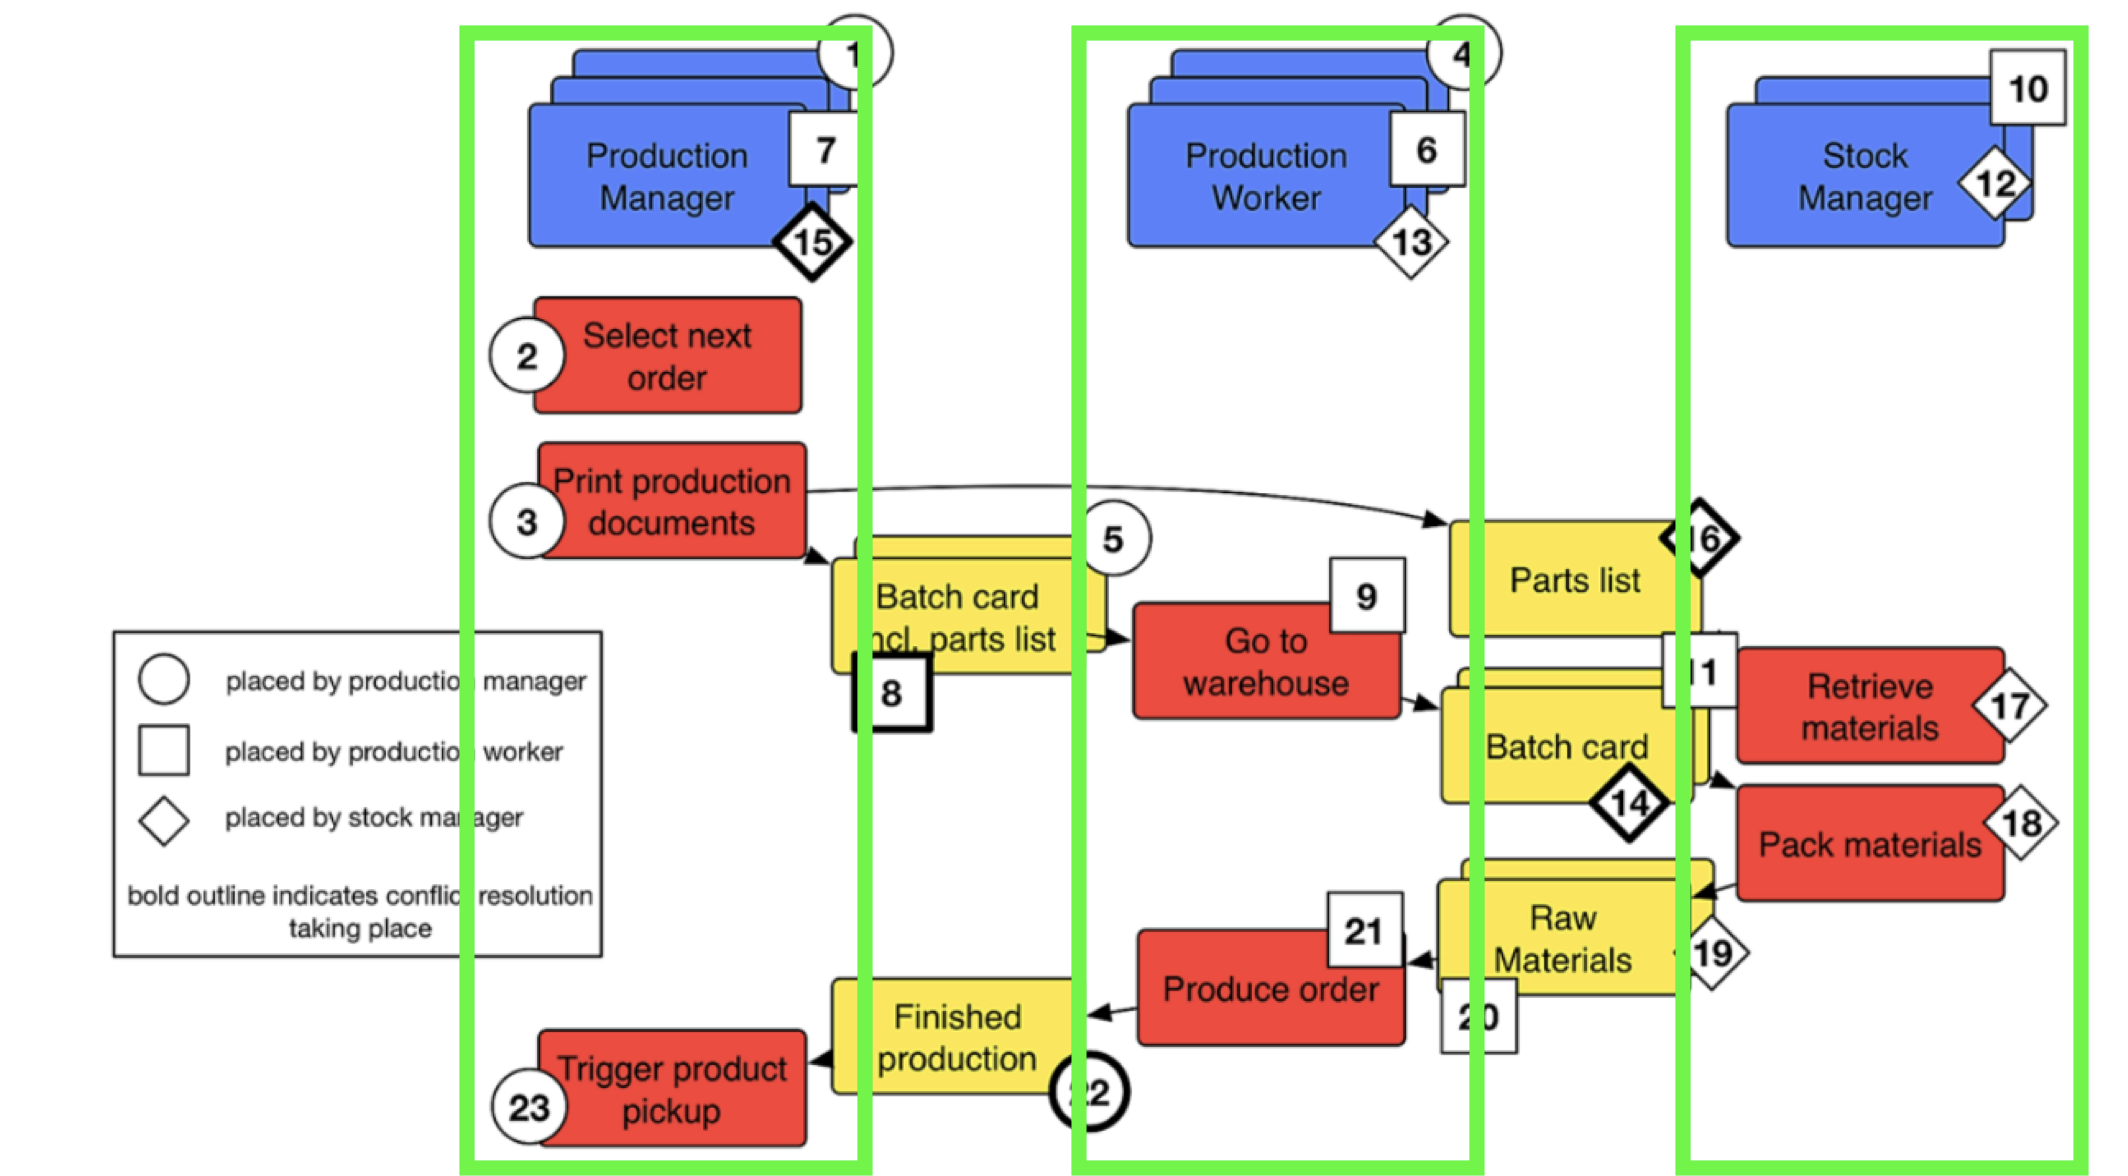
\includegraphics[width=\textwidth]{figures/cbm-grundstruktur.png}
		\caption[CBM Modell]{CBM Modell \protect~\cite{oppl2016linking}}
		\label{fig:cbm-grundstruktur} 
	\end{minipage}
\end{figure}
% chapter hintergrund (end)
%----------------------------------------------------------------
%
%  File    :  empfehlungen.tex
%
%  Author  :  Thomas Fragner
% 
%  Created :  2017-10-01
% 
%  Changed :  2018-04-10
% 
%----------------------------------------------------------------

\chapter{Verständlichkeit von CBM-Modellen}
\label{cha:Empfehlungen}
In diesem Kapitel wird die erste Forschungsaufgabe behandelt. Die Methode CBM \citep{Oppl:2015:ASB:2723839.2723841} wird auf die einfache Verständlichkeit der Notation unter Berücksichtigung der zugrundeliegenden Modellierungsvorschriften überprüft.

\citeauthor{MENDLING2010127} definieren die folgenden Kriterien, welche zur einfachen Verständlichkeit von Prozessmodellen erfüllt werden sollten:
\begin{enumerate}
	\item G1 Verwendung soweniger Elemente wie möglich.
	\item G2 Geringe Anzahl der ein- und ausgehenden Verbindungen pro Element.
	\item G3 Ein Anfangs- und Endelement.
	\item G4 Strukturiertheit des Modells.
	\item G5 Vermeidung von ODER Verzweigungen.
	\item G6 Verwendung von Verb/Objekt Beschreibungen.
	\item G7 Dekomposition bei mehr als 50 Elementen.\citep{MENDLING2010127}
\end{enumerate}

Folegend wird für die einzelnen Punkte beschrieben inwiefern diese beim Card Based Modeling zutreffend sind bzw. erfüllt werden:

\begin{enumerate}
	\item wird erfüllt, da bei CBM meist auf einer höheren Abstraktionsebene modelliert wird, und die Möglichkeiten von Verzweigungen nicht vorgesehen sind. Daraus folgt, dass die potenzielle Anzahl von Elementen in einem CBM Modell niedrig ist. Weiter wird die Anzahl meist durch die beschränkten Platzverhältnisse beim Modellieren beeinflusst. 
	\item wird erfüllt, da es sich um ein sequenzielles Modell handelt und damit verbunden gibt es im Normalfall nur einen Ein- bzw. Ausgang pro Aufgabe.
	\item wird erfüllt, da aufgrund der sequenziellen Natur der Modellierungssprache meist nur ein Start- bzw. Endelement existiert.
	\item wird erfüllt, da es keine Notationselemente zum Verzweigen (Gateways) des Prozesspfades gibt. 
	\item wird erfüllt, da es kein entsprechendes Notationselement gibt. 
	\item kann erfüllt werden, da es sich hierbei um eine formale Richtlinie handelt.
	\item Die siebte Regel ist unabhängig von der verwendeten Notation und kann in jedem Fall erfüllt werden.
\end{enumerate}

Die Analyse von CBM nach den Regeln von \citet{MENDLING2010127} legt nahe, dass CBM für das Verständnis durch die beteiligten Personen sehr gut geeignet ist. Wie in der Einleitung bereits beschrieben, ist jedoch eine digitale Repräsentation der gelegten Prozessmodelle eine wichtiger Aspekt um die Weiterverwendung zu gewährleisten. Im folgenden Kapitel wird beschrieben welche Konstellationen, basierend auf den Testbeispielen von \citet{max}, bei der Analyse berücksichtigt werden sollen.


%----------------------------------------------------------------
%
%  File    :  analyse.tex
%
%  Author  :  Thomas Fragner
% 
%  Created :  2017-10-01
% 
%  Changed :  2018-04-10
% 
%----------------------------------------------------------------

\chapter{Erkennung sequenzieller Legestrukturen} % (fold)
\label{cha:erkennung}
Nachdem in Kapitel \ref{cha:hintergrund} die Grundlage zum Verständnis von sequenziell gelegten Prozessen in CMB Modellen  dargestellt wurde, werden in diesem Kapitel das notwendige Ausgangsmaterial, die Kriterien bzw. die Strategie zur Erkennung dieser Strukturen untersucht. Diese Erkenntnisse bilden die Basis für den Algorithmus.

\section{Allgemeine Einschränkung} % (fold)
\label{sec:allgmeine_einschrankung}
Der zu entwickelnde Algorithmus kann nur Strukturen erkennen, die auch ein Mensch ohne genaue inhaltliche Kenntnisse des Prozesses ableiten kann. Das heißt, dass nur geometrische Anordnungen bei der Erkennung berücksichtigt werden. Diese Anordnungen müssen im weitesten Sinne einen linearen sequenziellen Zusammenhang erkennen lassen.
% section allgmeine_einschrankung (end)

\section{Ausgangsmaterial} % (fold)
\label{sec:ausgangsmeterial}
Der Algorithmus verarbeitet nicht das Basisbildmaterial direkt, sondern verwendet eine bereits digitalisierte Repräsentation die durch den Model Digitizer \cite{opplstary2017}, welcher Bildmaterial in SVG Grafiken umwandelt, erzeugt wird.

Folgende Daten werden vom Model Digitizer pro Karte zur Verfügung gestellt und dienen als Eingangsdaten für den Algorithmus:
\begin{itemize}
	\item eindeutige Karten-ID
	\item Kartentyp
	\begin{itemize}
		\item Subjekt
		\item Aufgabe
		\item Austausch
	\end{itemize}
	\item X- und Y-Koordinaten für die Eckpunkte der Karte. 
\end{itemize}
% section ausgangsmeterial (end)

\section{Problemstellungen} % (fold)
\label{sec:problemstellungen}
Bei der algorithmischen Auswertung sequenzieller Abfolgen ergeben sich 4 Hauptkriterien, welche bei der Interpretation berücksichtigt werden müssen:
\begin{enumerate}
	\item Abweichungen von den Legevorschriften laut CBM.
	\item Ungenaue Positionierung der Karten.
	\item Unterschiedliches Ausgangsbildmaterial.
	\item Fehlerhafte Interpretation durch den Model Digitizer.
\end{enumerate}

\subsection{Abweichungen von den Legevorschriften} % (fold)
\label{ssub:abweichung_von_der_legevorschriften}
Basierend auf den Testbeispielen \cite{max} ergeben sich Abweichungen, die eine algorithmische Verarbeitung der Daten unmöglich machen oder erschweren.

Aus den Testbeispielen haben sich zwei grundsätzliche Legemuster ergeben:

\begin{itemize}
	\item Linienlayout (siehe Abbildung ~\ref{fig:linienlegemethode}) 
	\item Sternlayout (siehe Abbildung ~\ref{fig:sternlegemethode}) 
\end{itemize}

\begin{figure}[h]
	\centering 
	\begin{minipage}[b]{0.45\textwidth} 
		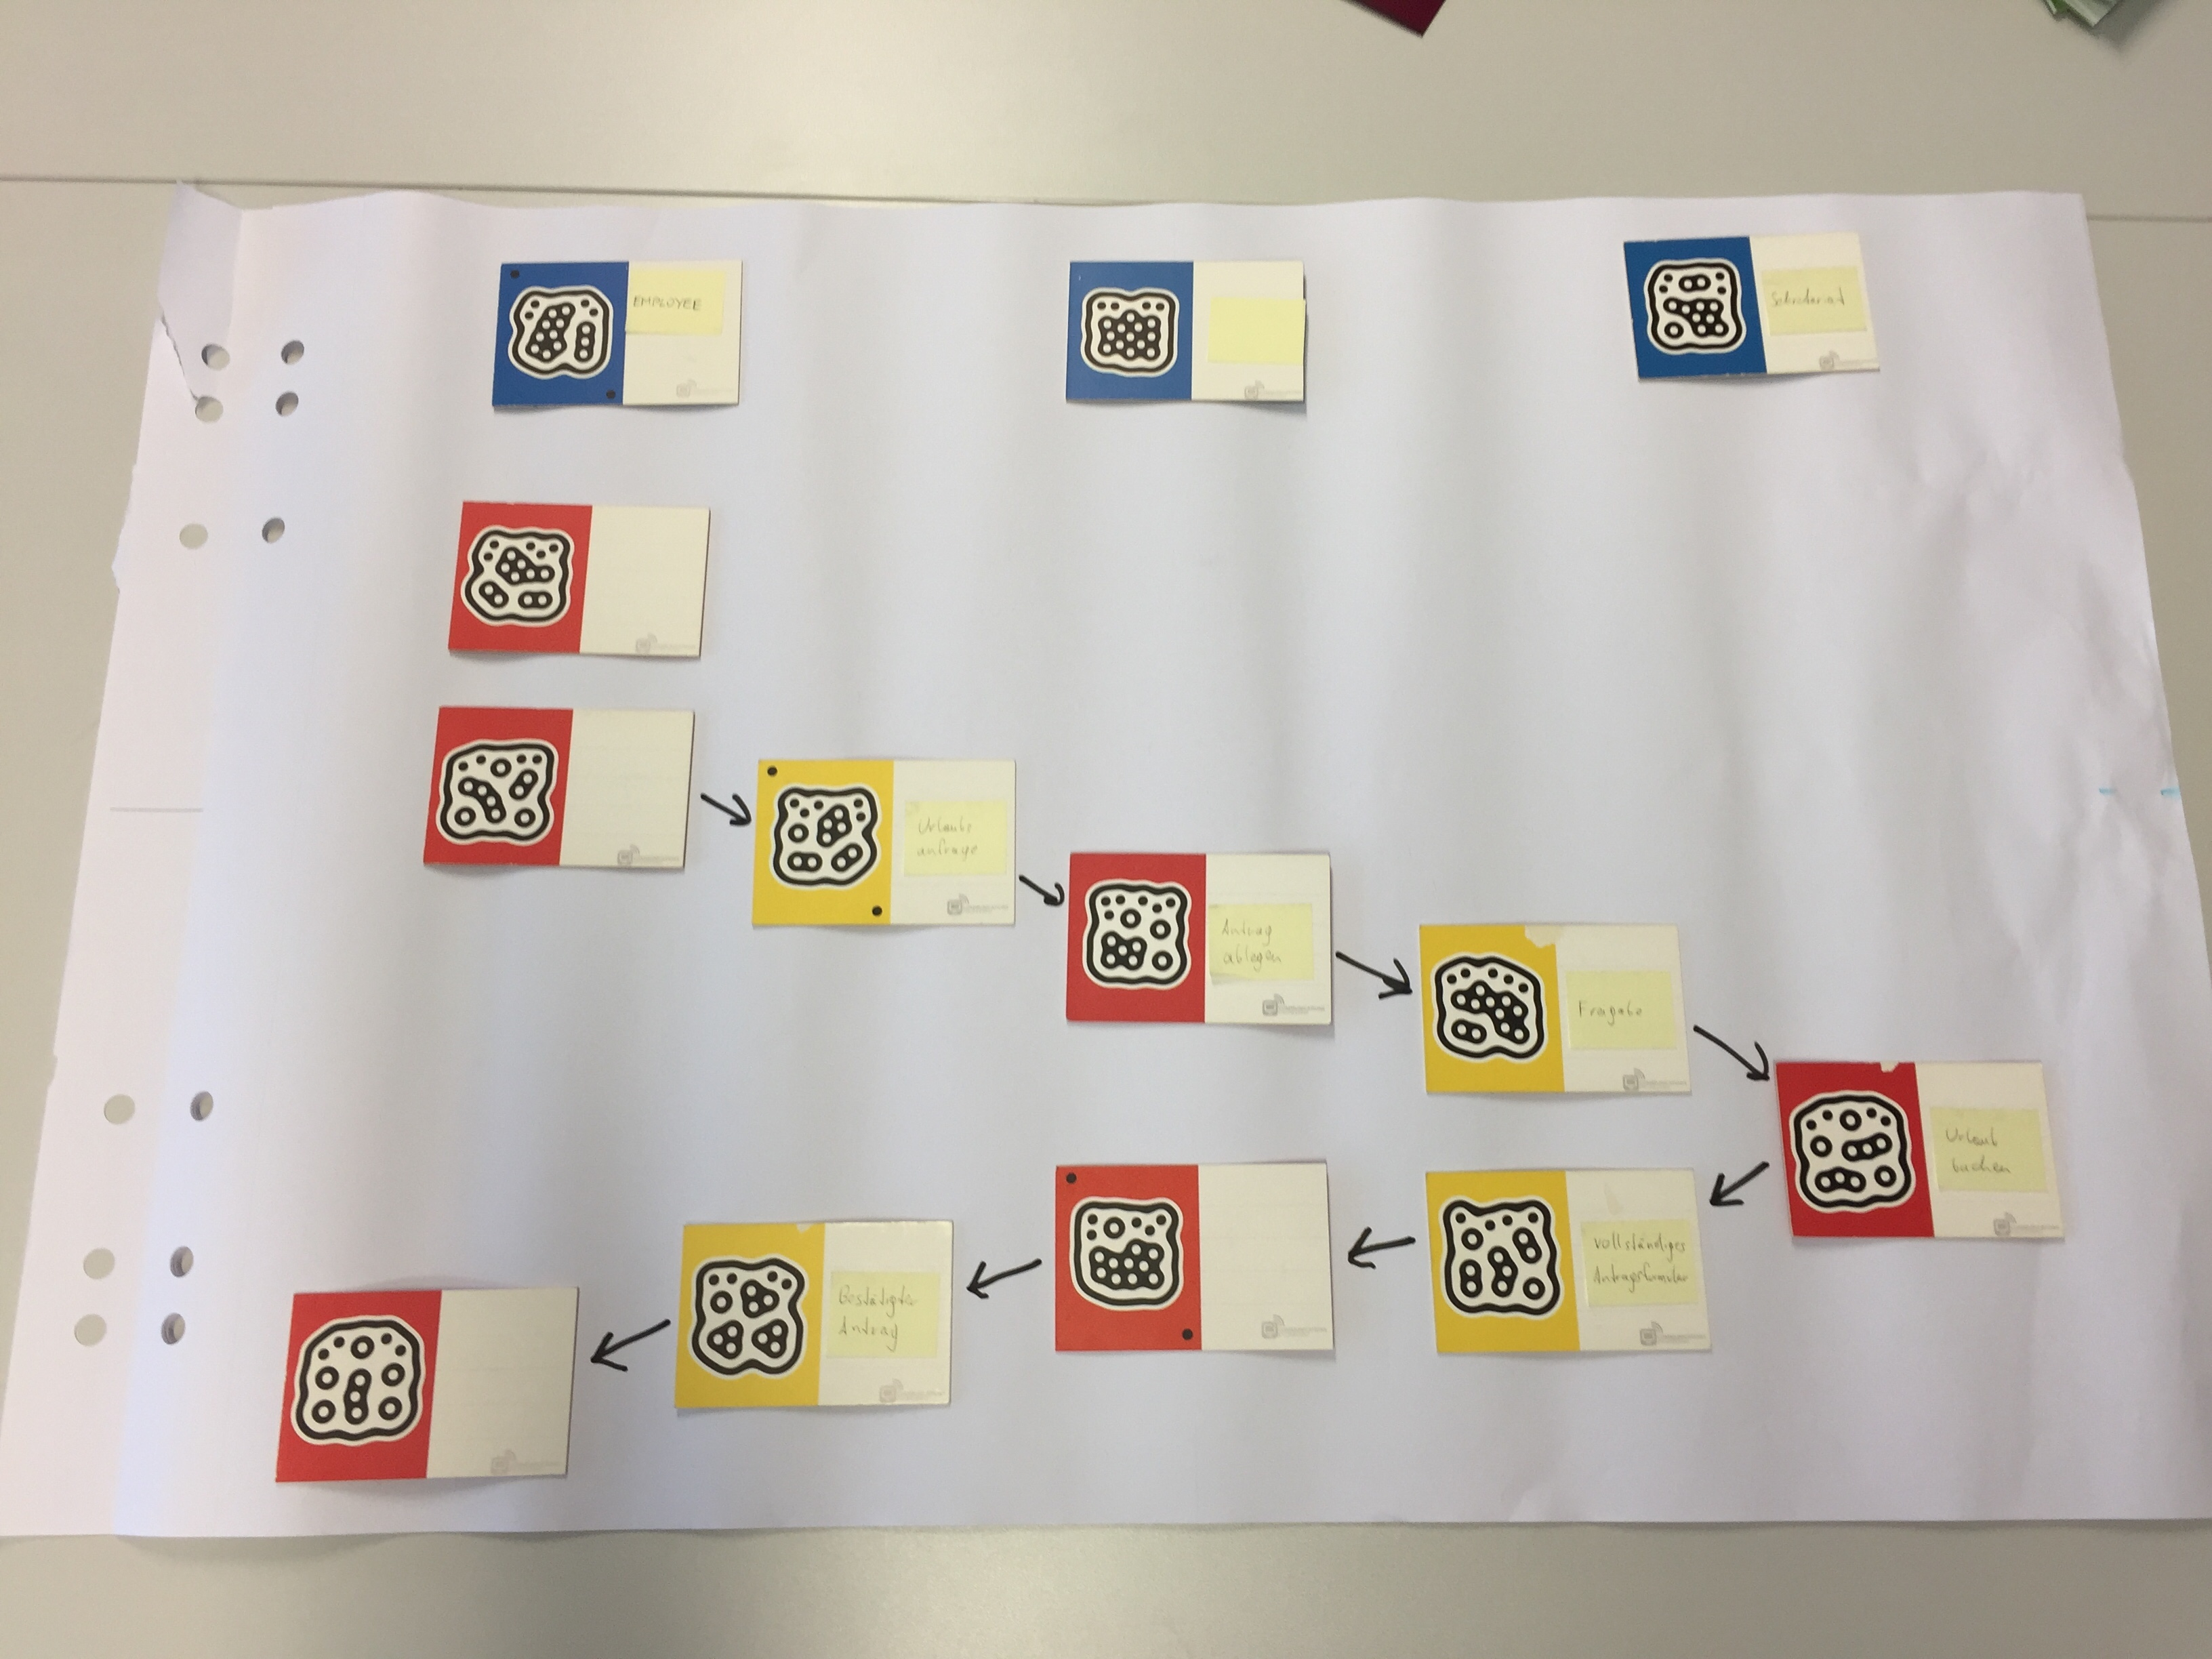
\includegraphics[width=\textwidth]{figures/linienlegemethode.jpg}
		\caption{Linienlayout  \protect~\cite{max}} 
		\label{fig:linienlegemethode} 
	\end{minipage}
	\hfill 
	\begin{minipage}[b]{0.45\textwidth} 
		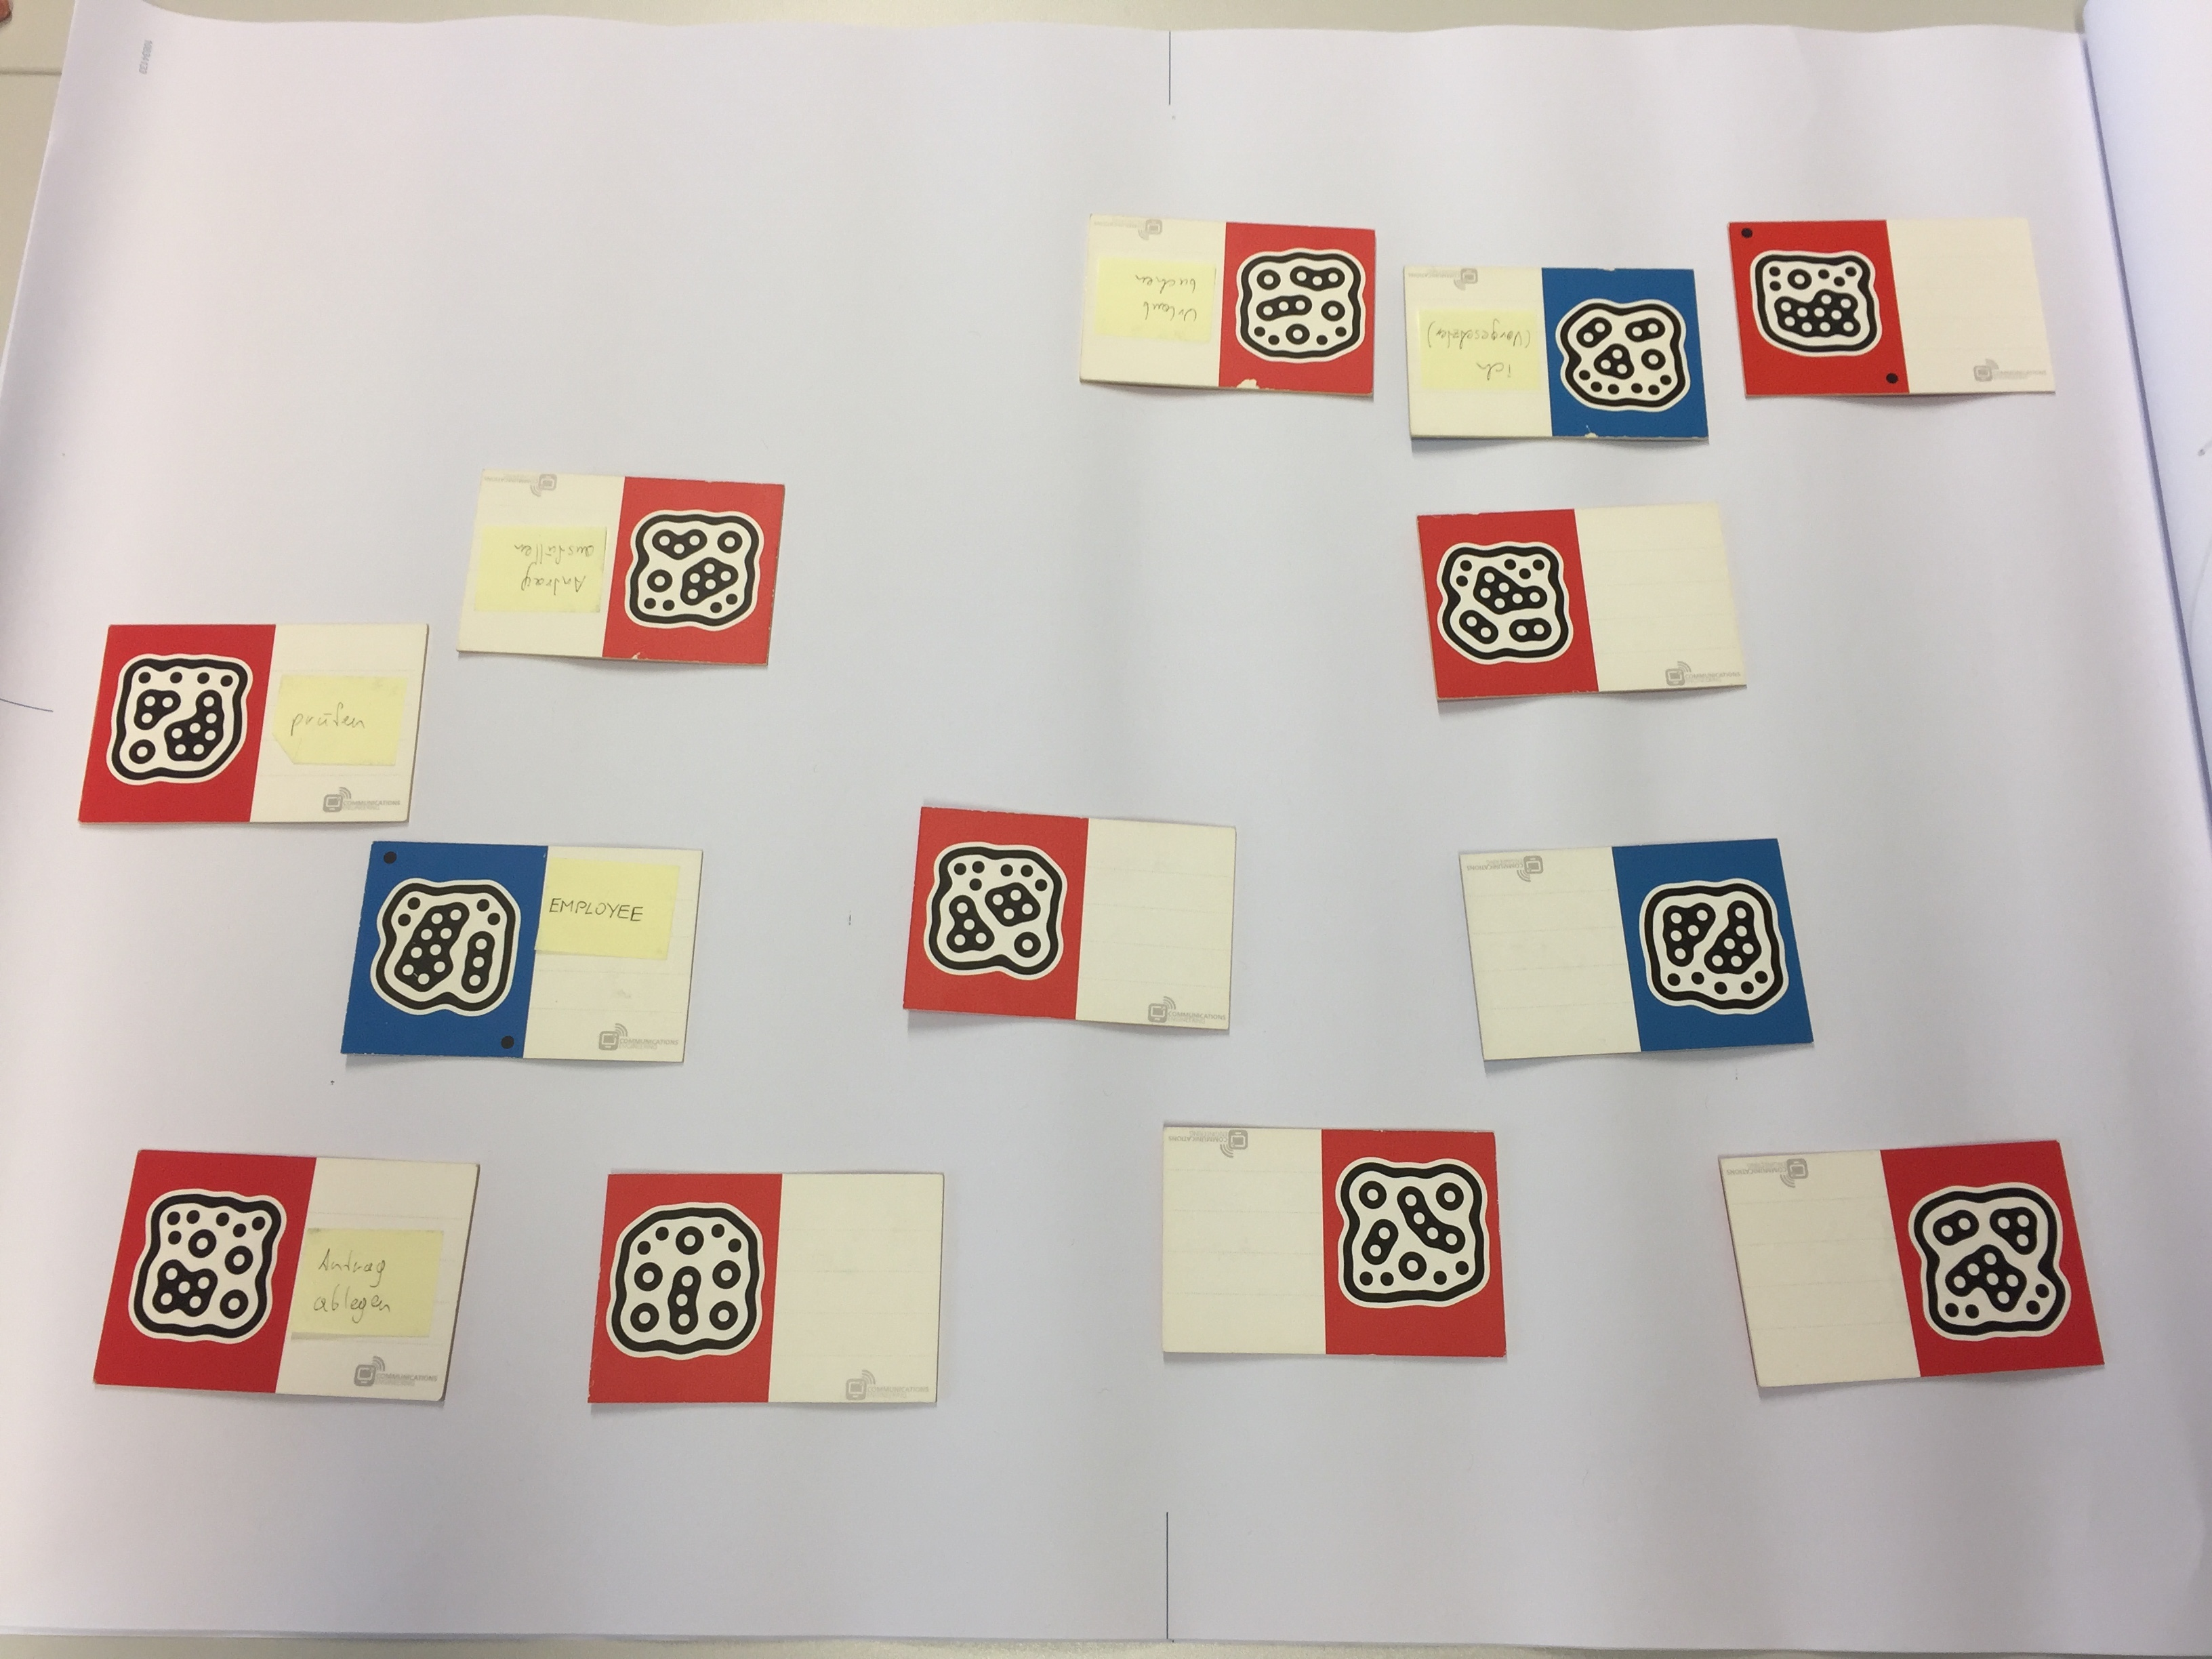
\includegraphics[width=\textwidth]{figures/sternlegemethode.jpg} 		\caption{Sternlayout 
		\protect~\cite{max}} 
		\label{fig:sternlegemethode} 
	\end{minipage}
\end{figure}

Das Linienlayout entspricht den vorgegebenen Legevorschriften. Beim Sternlayout werden die Vorschriften nicht beachtet. Es ergeben sich daraus folgende Problemstellungen:
\begin{itemize}
	\item Es kann kein Startelement erkannt werden, da alle Aufgaben annähernd gleich weit vom nächstgelegenem Subjekt entfernt sind.
	\item Es ist keine sequenzielle Struktur ausgehend vom Subjekt erkennbar, und daher kann kein chronologischer Zusammenhang zwischen den Aufgaben abgeleitet werden.
\end{itemize}

Aufgrund dieser Merkmale ist das Sternlayout nicht zur Analyse geeignet, aber es ergibt sich die Anforderung diese beiden Layouttypen voneinander unterscheiden zu können.

Eine weitere Abweichung betrifft die Anordnung der Subjekte und die Legerichtung der Aufgaben. In Abbildung \ref{fig:subjekt-position} sind die Subjekte entgegen den Vorschriften nicht horizontal auf einer Linie am oberen Bildrand angeordnet. Abbildung \ref{fig:nicht-vertikal} zeigt, dass die Aufgaben nicht vertikal ausgehend vom Subjekt angeordnet sind.

Obwohl die Legevorschriften bei beiden Prozessmodellen nicht eingehalten werden, sind die chronologischen Subjekt/Aufgabe Zuordnungen klar ersichtlich. Diese Muster sollten vom Algorithmus daher richtig erkannt werden. 

\begin{figure}[h]
	\centering 
	\begin{minipage}[b]{0.45\textwidth} 
		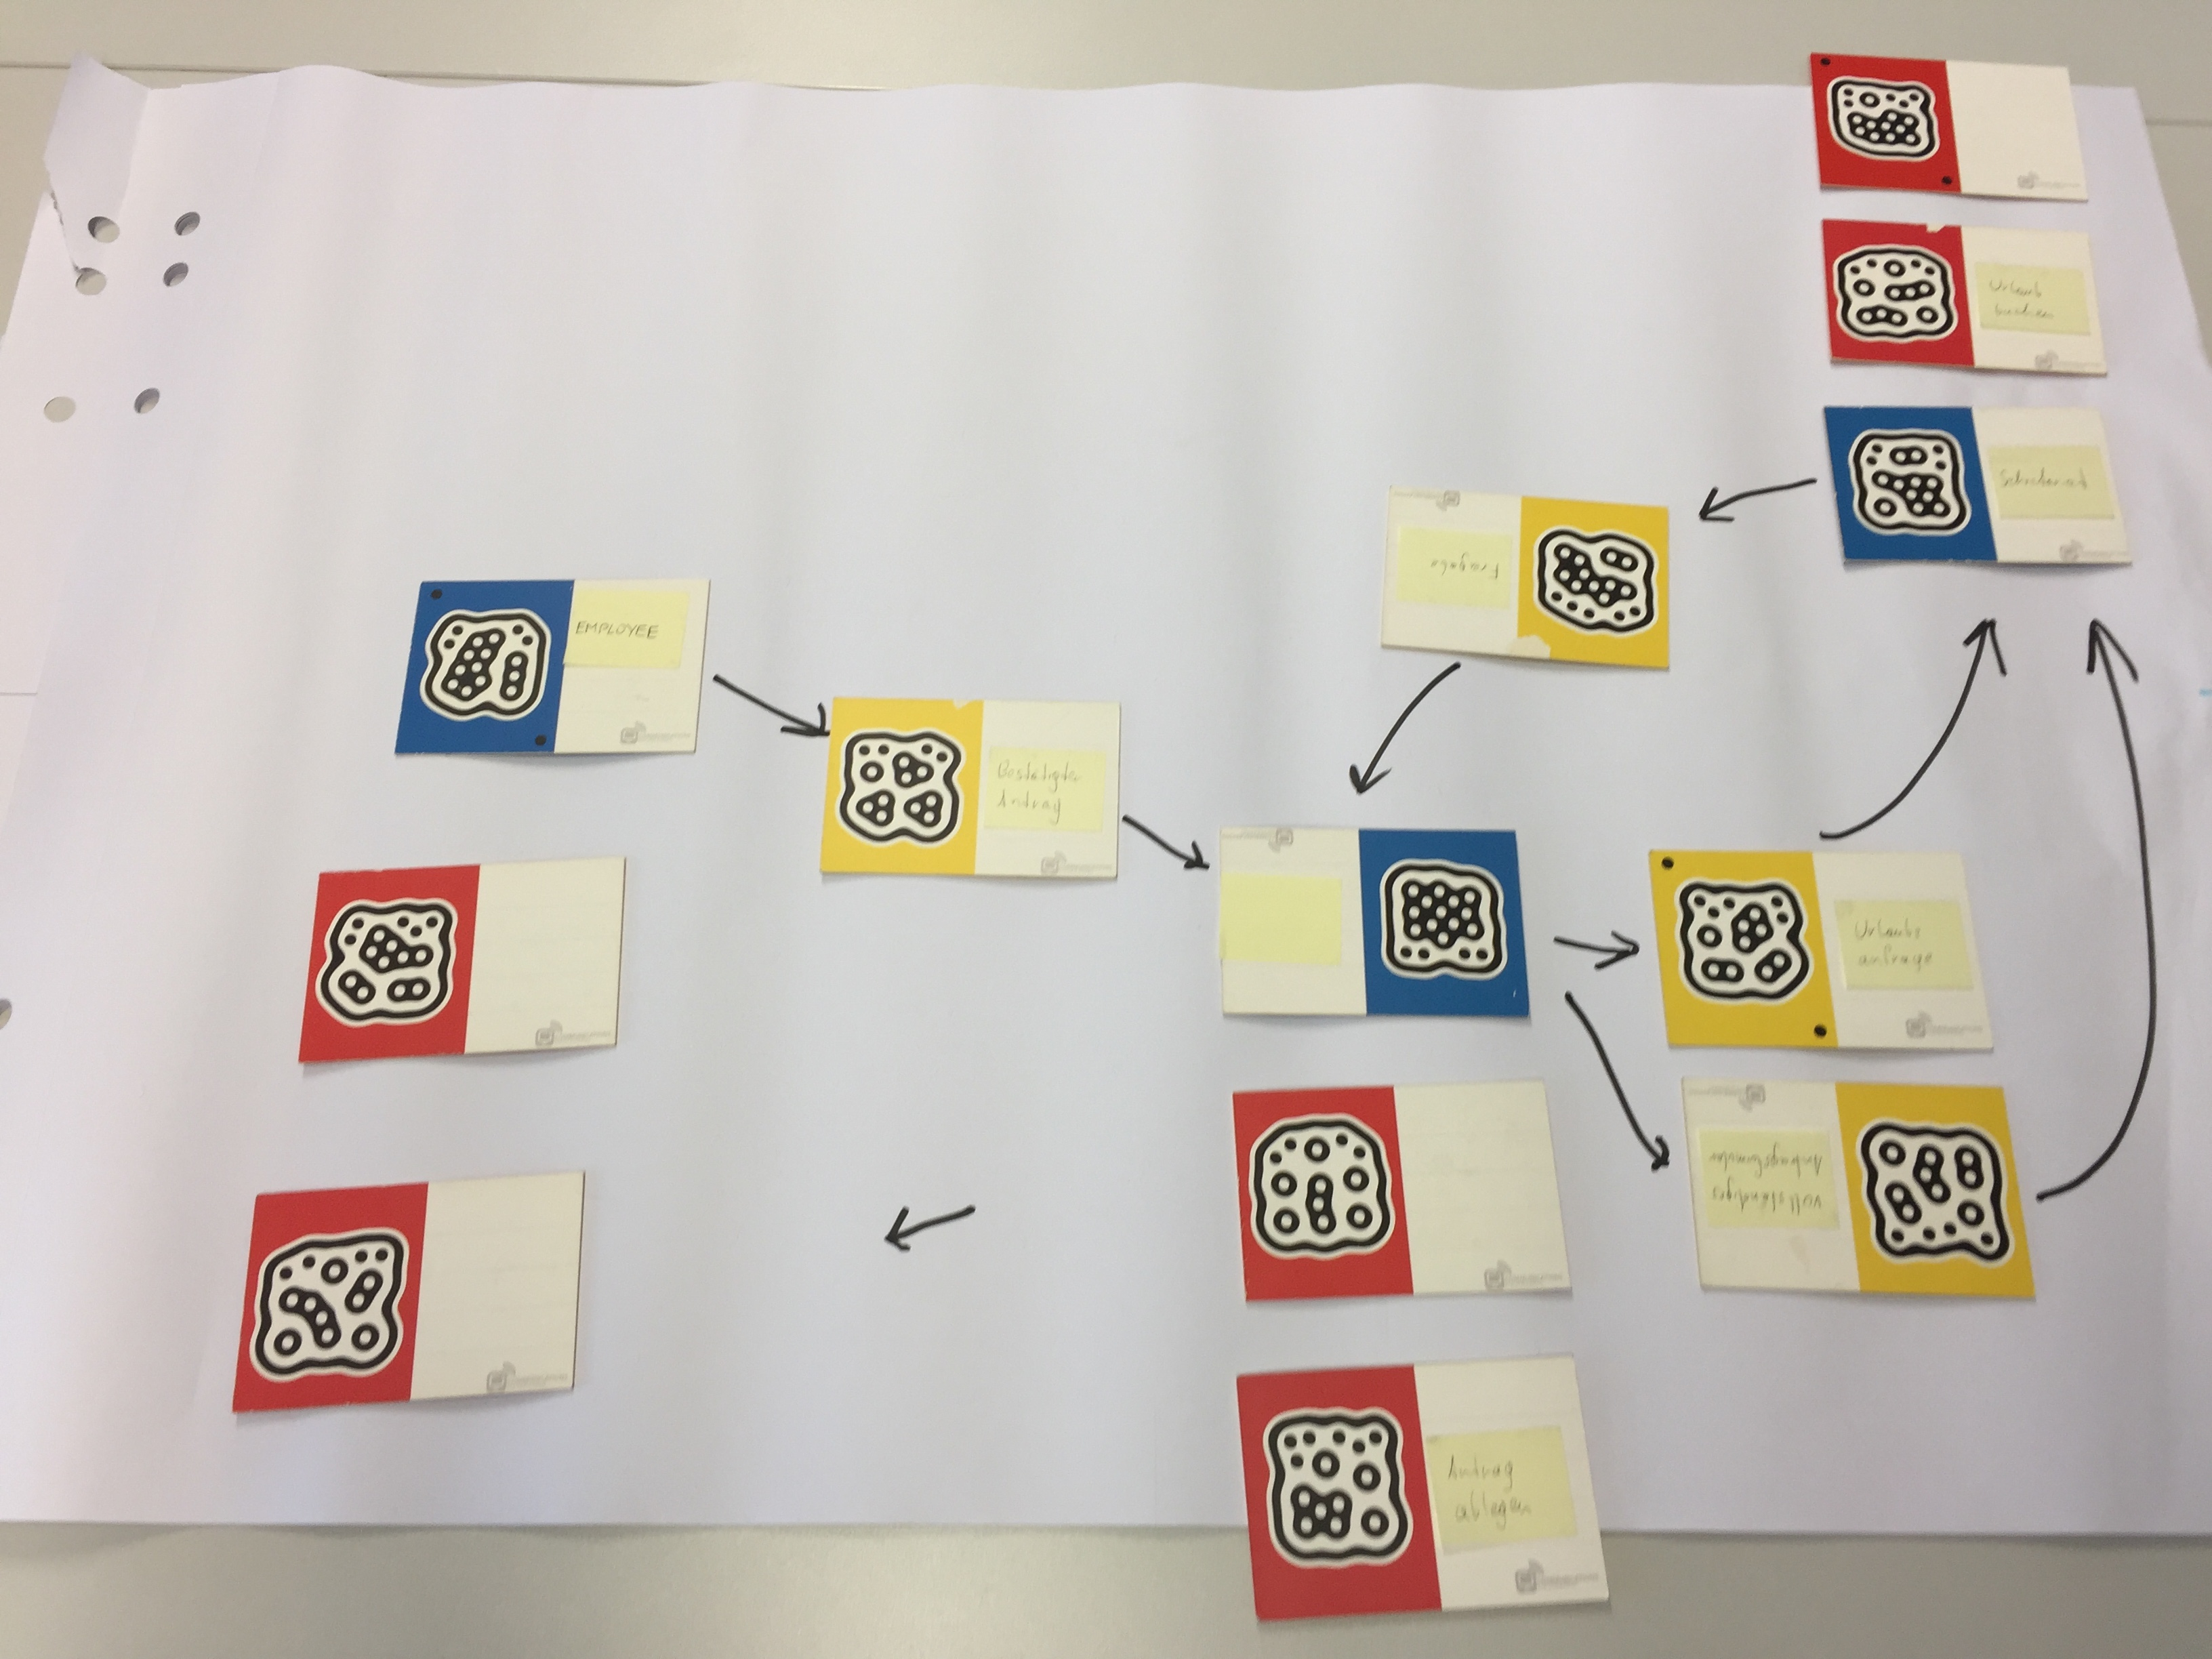
\includegraphics[width=\textwidth]{figures/03.jpg}
		\caption{Subjektposition \protect~\cite{max}} 
		\label{fig:subjekt-position} 
	\end{minipage}
	\hfill 
	\begin{minipage}[b]{0.45\textwidth} 
		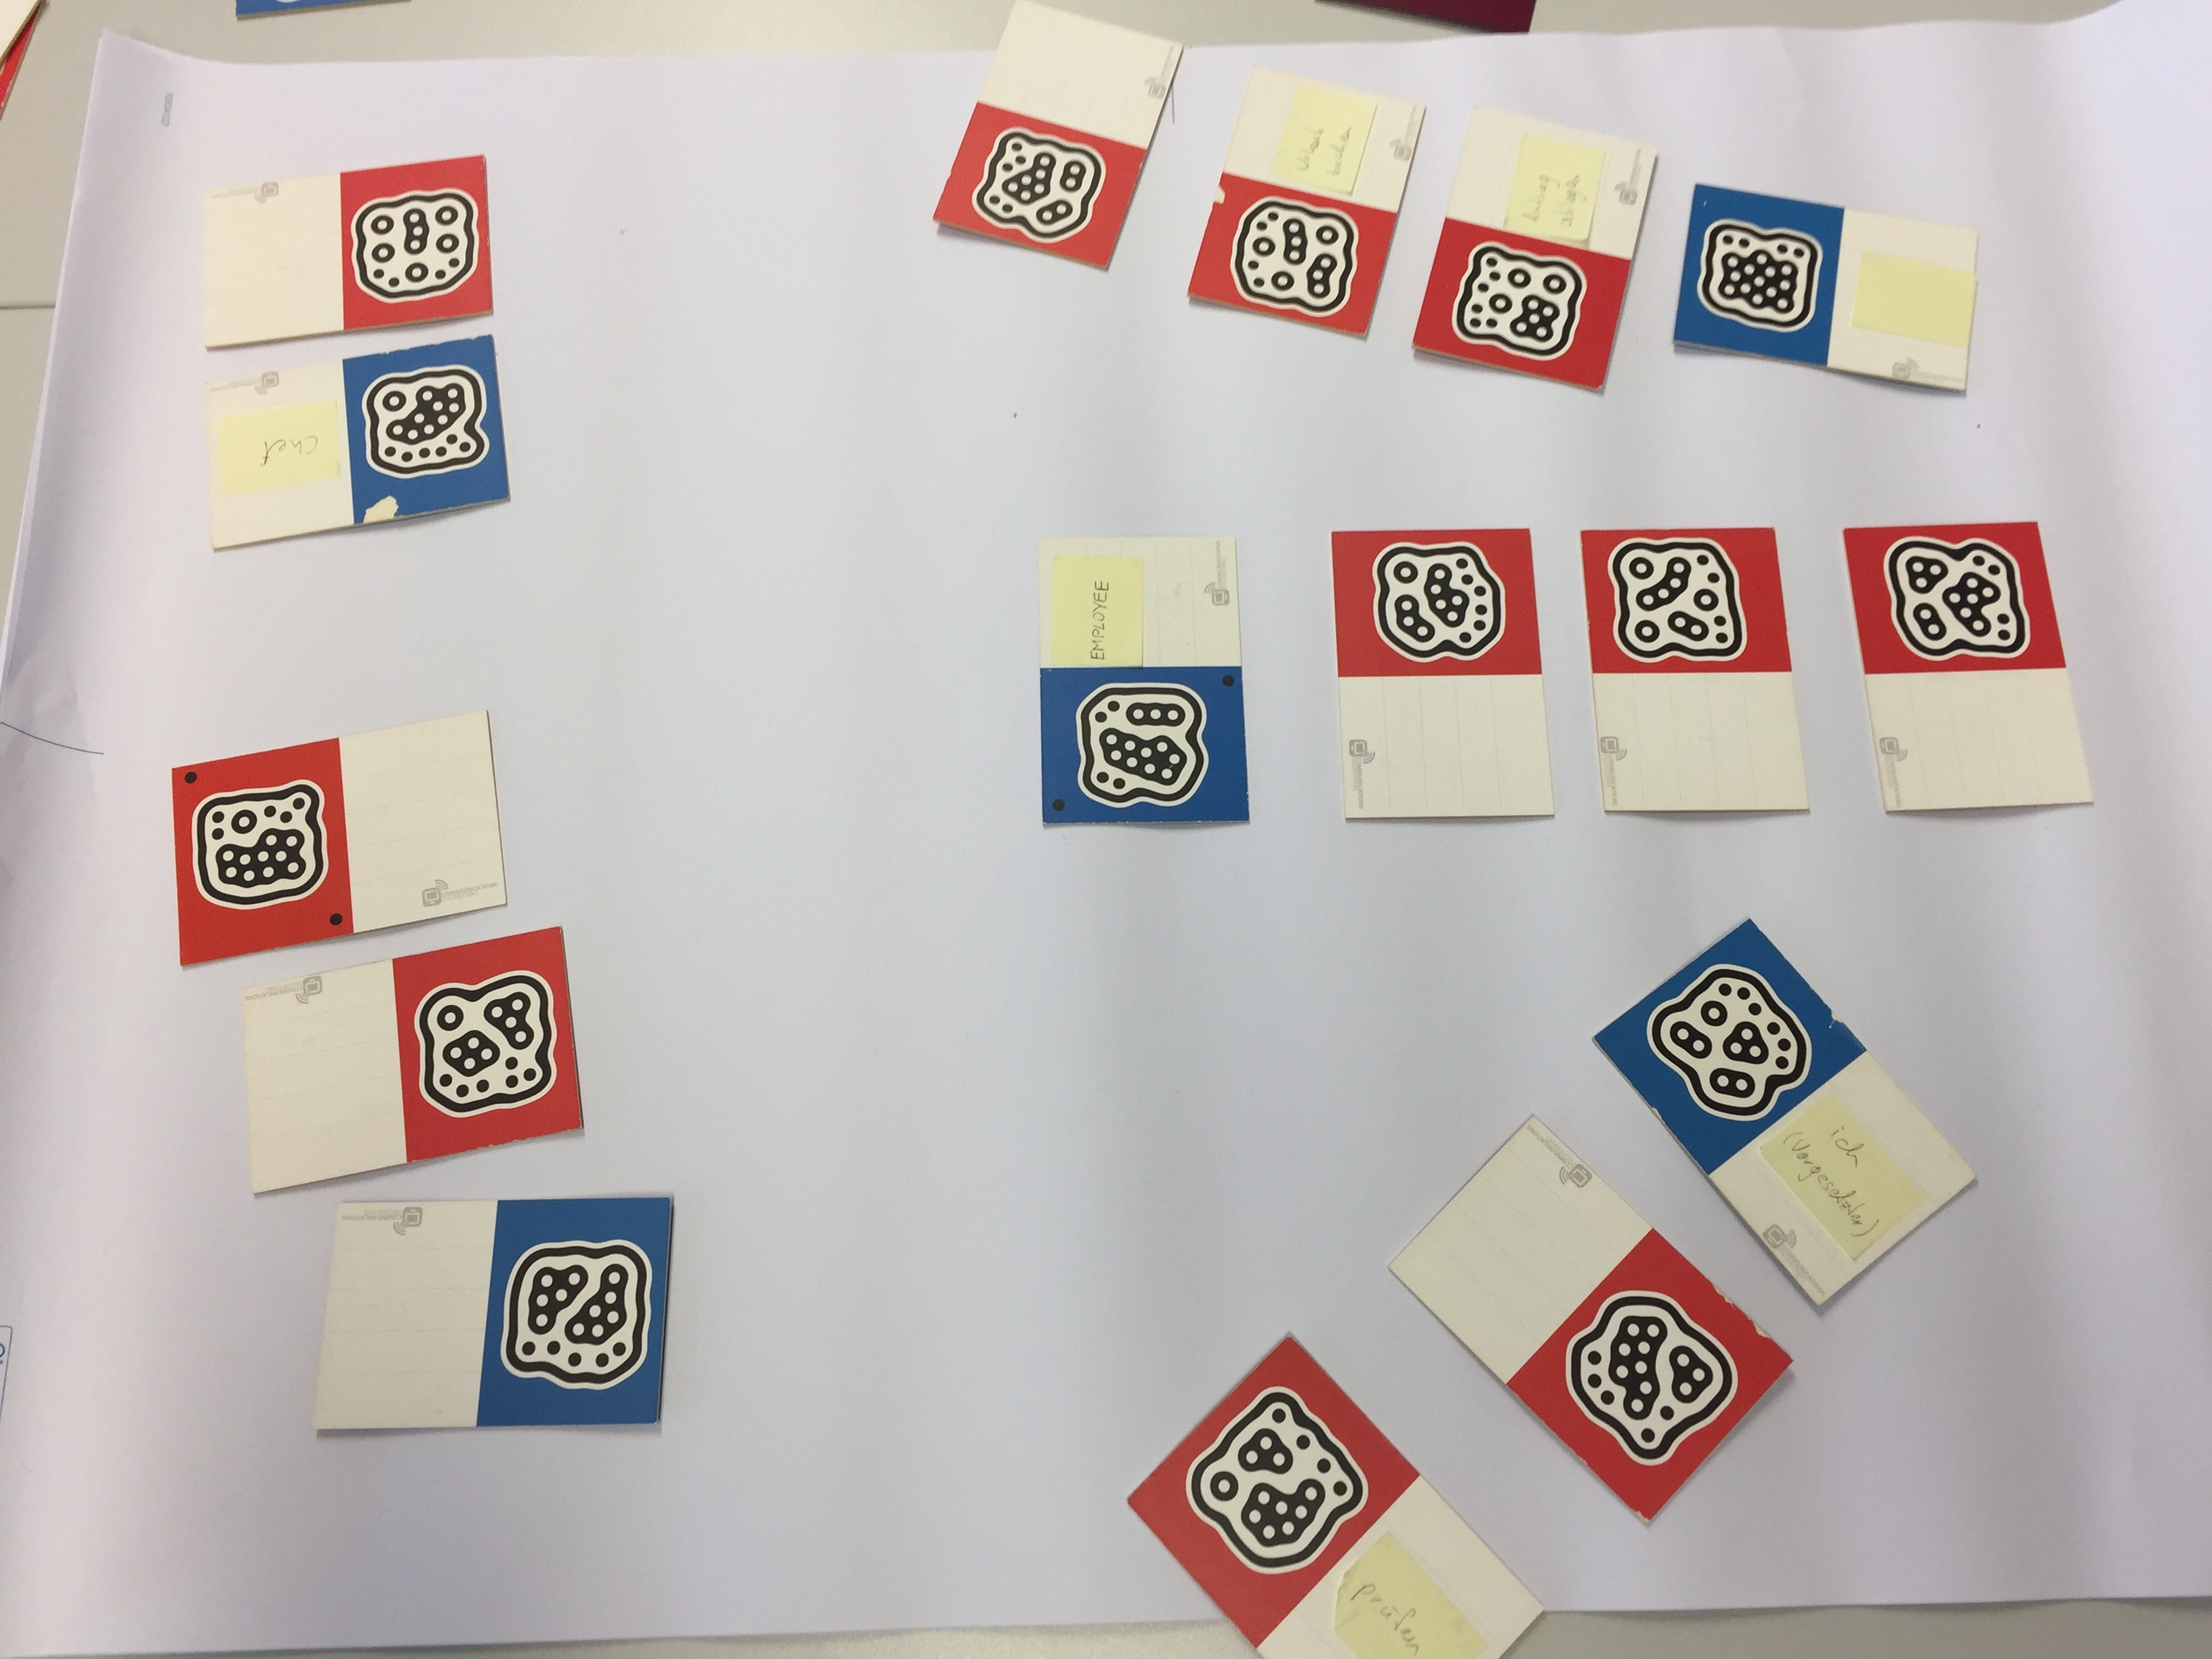
\includegraphics[width=\textwidth]{figures/17.jpg} 		
		\caption{Richtungsunterschiede \protect~\cite{max}} 
		\label{fig:nicht-vertikal} 
	\end{minipage}
\end{figure}
% subsubsection abweichung_von_der_legevorschrift (end)

\subsection{Ungenaue Kartenlegung} % (fold)
\label{ssub:ungenaue_kartenlegung}
Mit der Methode des Kartenlegens verbunden, ist die ungenaue Positionierung und Lage der Karten. In Abbildung \ref{fig:karten-position} ist ersichtlich, dass die roten Aufgabenkarten nicht exakt unterhalb des Subjekts angeordnet sind und auch eine Rotation dieser Karten feststellbar ist. Diese Ungenauigkeiten sollten vom Algorithmus innerhalb einer bestimmten Toleranz ebenfalls richtig interpretiert werden.

\begin{figure}[h]
	\centering 
	\begin{minipage}[b]{0.8\textwidth} 
		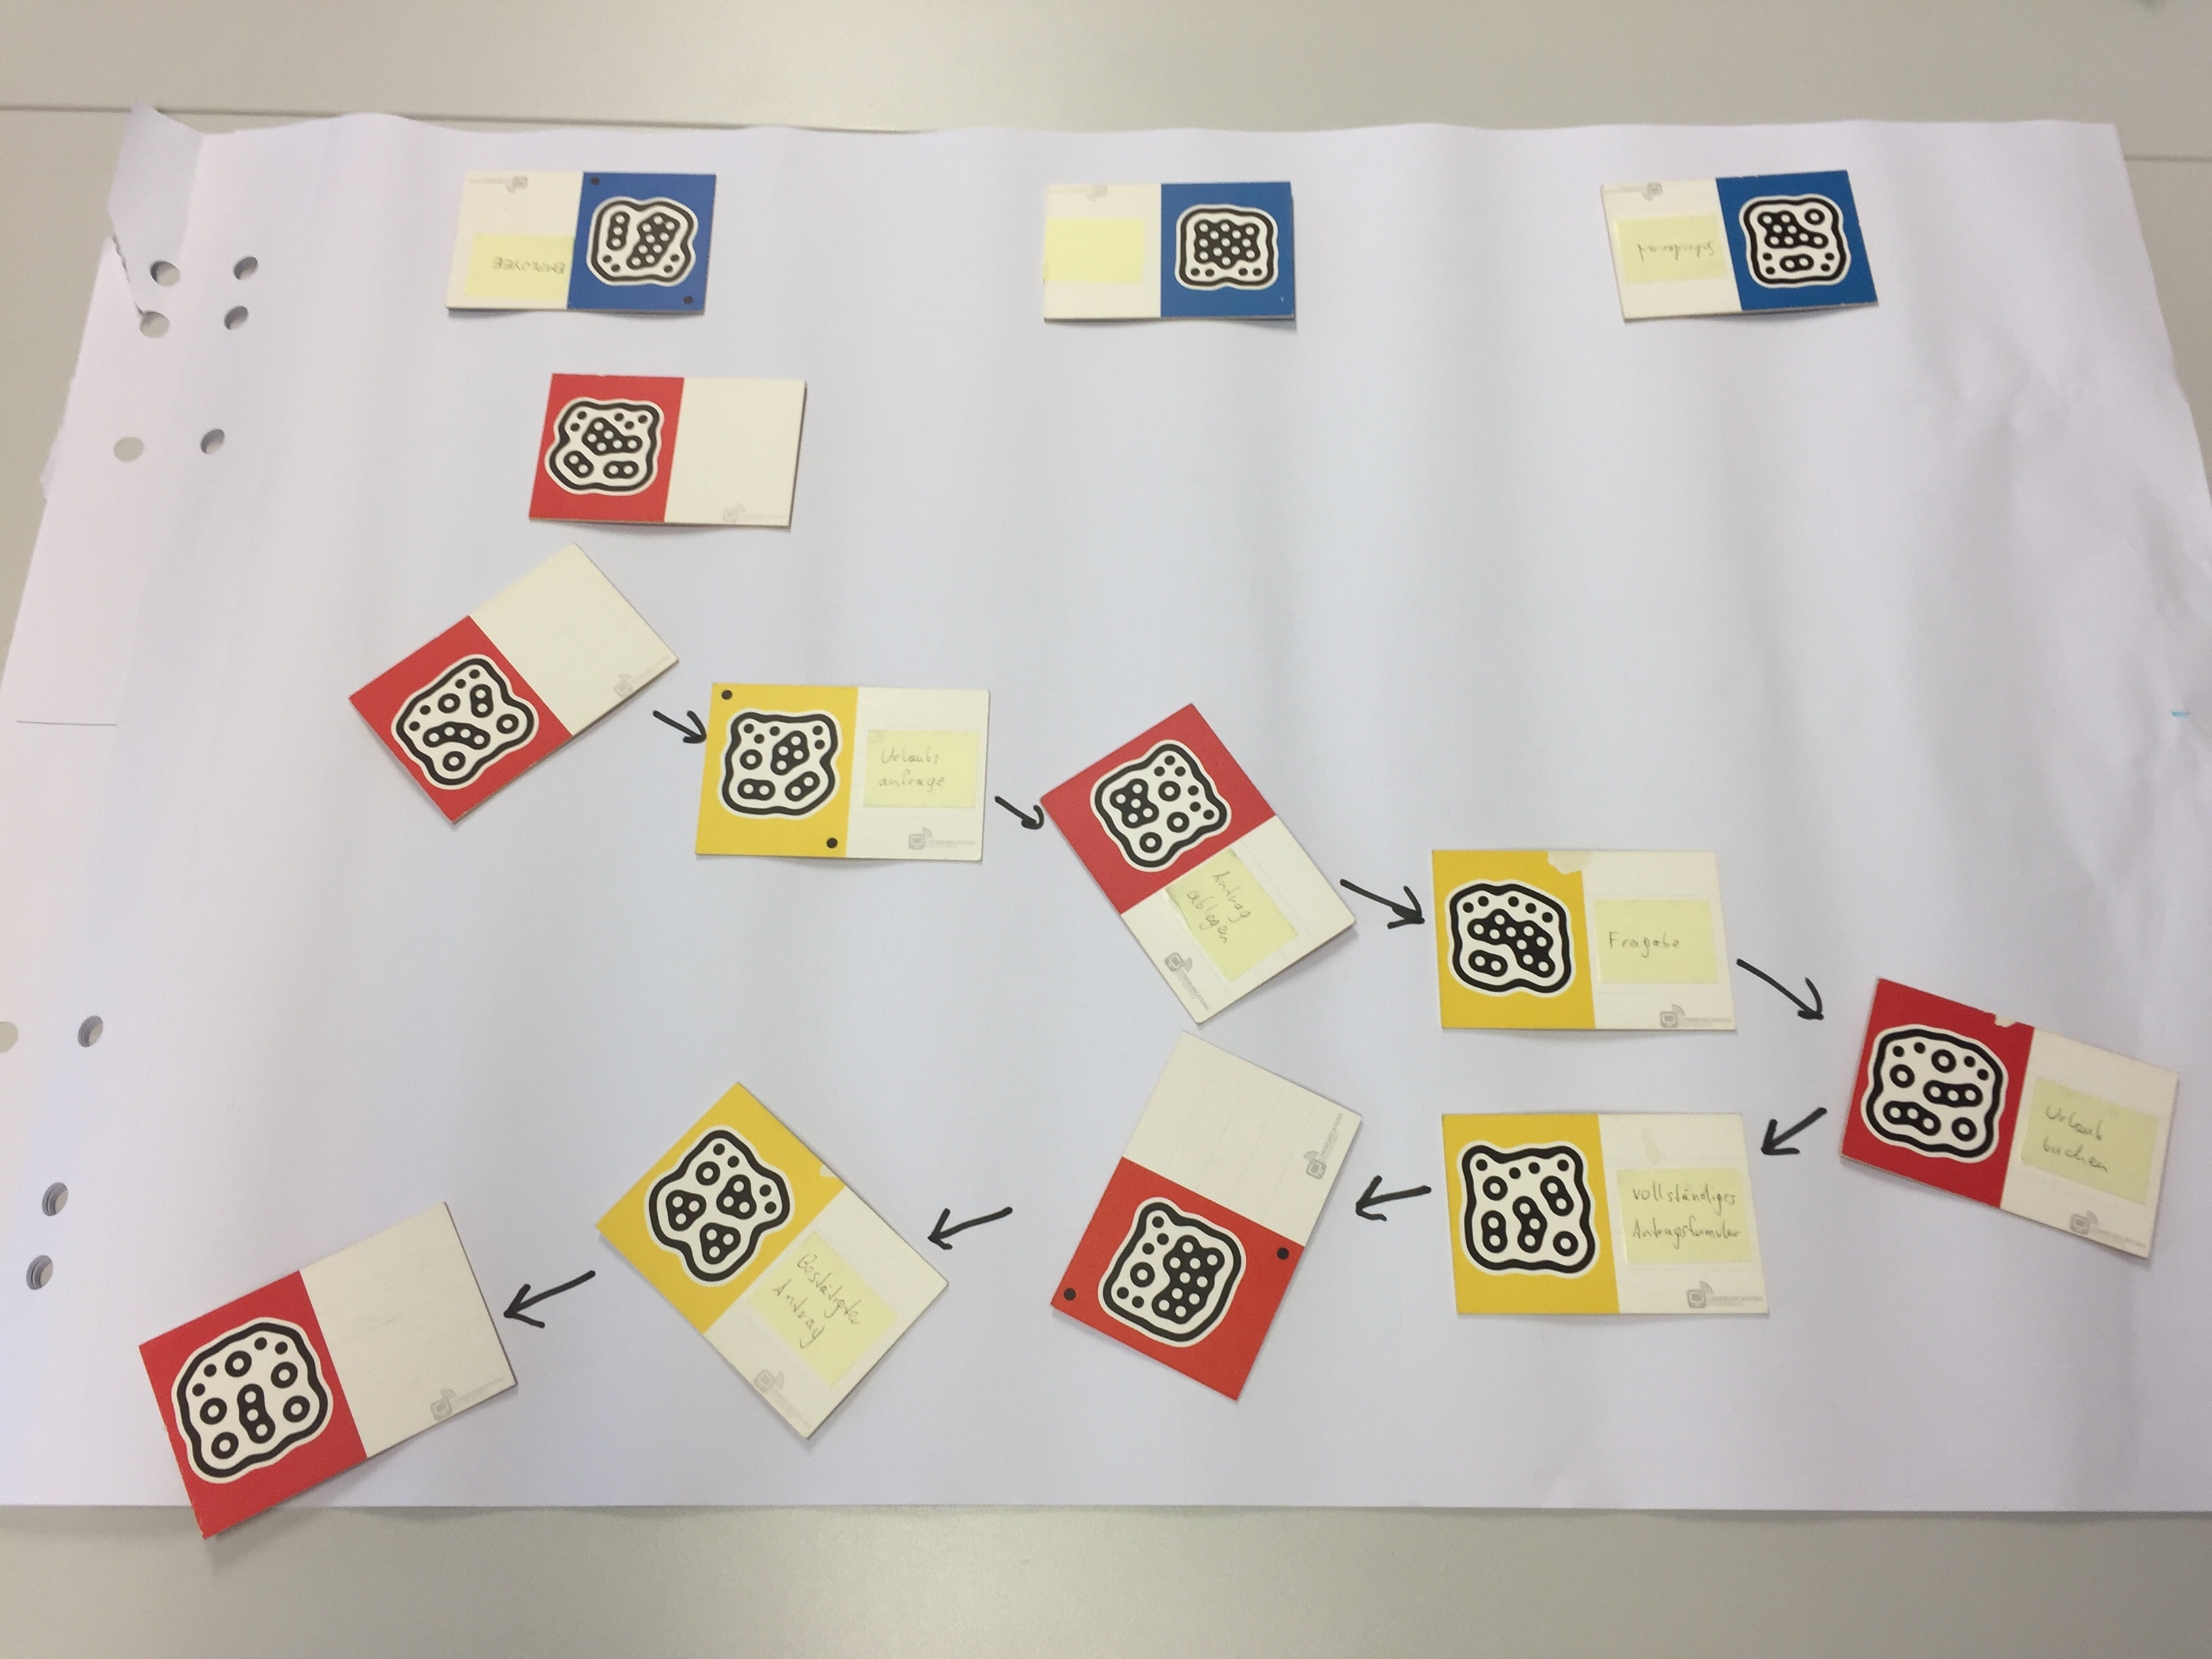
\includegraphics[width=\textwidth]{figures/02.jpg}
		\caption{Kartenposition und -orientierung  \protect~\cite{max}} 
		\label{fig:karten-position} 
	\end{minipage}
\end{figure}
% subsubsection ungenaue_kartenlegung (end)

\subsection{Ausgangsbildmaterial} % (fold)
\label{sub:ausgangsbildmaterial}
Im ersten Schritt der Digitalisierung wird mit Hilfe von digitalen Aufnahmegeräten ein Bild des Prozesses erstellt. Daraus ergeben sich mehrere Unterschiede im Ausgangsmaterial die potentiell Einfluss auf die algorithmische Auswertung haben:

\begin{itemize}
	\item Auflösung des Bildmaterials
	\item Perspektive der Aufnahme
	\item Bildqualität
\end{itemize}

Die Bildqualität verschlechtert das Ergebnis der Umwandlung in Vektorgrafiken mit Hilfe des Model Digitizer, und beeinflusst somit indirekt den Algorithmus. Die Auflösung bzw. Perspektive wirkt sich auf die Größe der Elemente aus und hat direkten Einfluss auf den Algorithmus. Daher soll der Algorithmus grundsätzlich mit unterschiedlichen Bildmaterialien umgehen können.
% subsection ausgangsbildmaterial (end)

\subsection{Fehlerhafte Basisdaten} % (fold)
\label{sub:fehlerhafte_basisdaten}
Für die Erkennung der sequenziellen Strukturen wird auf eine bereits digitalisierte Version der Rohdaten zugegriffen. Daraus ergibt sich, dass eventuelle Fehler im ersten Digitalisierungsschritt Auswirkungen auf den Algorithmus haben. In den folgenden Kapiteln wird davon ausgegangen, dass die vorhandenen Daten vollständig und richtig sind.
% subsection fehlerhafte_basisdaten (end)
% section problemstellungen (end)

%Die Bilddaten müssen bereits in digitalisierter Struktur vorhanden sein. Dazu kann Bilderkennung und daraus abgleitet eine Vektorgrafik verwendet werden. Diese Vektorgrafik muss im Fall von CBM mindestens die folgenden Grunddaten enhalten.

\section{Erkennungsstrategie} % (fold)
\label{sec:erkennungsstrategie}
Aus den gewonnenen Erkenntnissen (siehe Kapitel \ref{sec:problemstellungen}) und dem bestehenden Algorithmus \cite{max} wird eine grundlegende Strategie zur Erkennung von sequenziell gelegten Prozessen vorgestellt, die als Basis für den Algorithmus dient.

\subsection{Bestehender Algorithmus} % (fold)
\label{sub:unterscheidung_der_legemethode}

% subsection unterscheidung_der_legemethode (end)
\citet{max} schlägt für die Erkennung der Abhängigkeiten die folgenden Algorithmusbestandteile vor:
\begin{description}
	\item[Euklidischer Abstand] Die Aufgaben werden dem Subjekt zugeordnet, zu dem die Aufgabe den geringsten Abstand aufweist.
	\item[Klassifizierung über Quadranten] Für jedes Subjekt werden Quadranten gebildet, und die Aufgaben werden dem Subjekt zugeordnet in dessen Quadrant die Aufgabe liegt.
	\item[Kombination] Die beiden zuvor genannten Methoden werden kombiniert betrachtet um mögliche Falschzuweisungen zu ermitteln.
	\item[Chronologische Ordnung] der Aufgaben wird durch die Abstände zum Subjekt bestimmt.
\end{description}

Zur Verbesserung der Erkennungsgenauigkeit sind weitere Kriterien bzw. Annahmen für die Zuweisungsbestimmung notwendig und werden in den folgenden Kapiteln beschrieben.

\subsection{Anfangselement} % (fold)
\label{sub:anfangselement}
Als Einstiegspunkt für den Algorithmus muss eine Subjekt/Aufgabe Kombination ermittelt werden. Die Kombination mit dem geringsten Abstand zwischen Subjekt und Aufgabe ist der wahrscheinlichste Start des Prozesses und somit der beste Ausgangspunkt um die weiteren Abhängigkeiten zu bestimmen.
\subsection{Richtungsbestimmung} % (fold)
\label{sub:richtungsbestimmung}
Bei einer sequenziell gelegten Anordnung ist eine annähernd gleiche Richtung der Aufgaben zu ihrem Startelement eine Bedingung. Diese Bedingung wurde beim bisherigen Ansatz nur teilweise bei der Klassifizierung nach Quadranten berücksichtigt, wobei diese Methode nur eine definierte Richtung berücksichtigt. Der euklidische Abstand beinhaltet keine derartige Information. Um diese Bedingung abbilden zu können ist eine weitere Metrik notwendig. Es wird die Verwendung der Kosinusähnlichkeit (siehe Formel  \ref{eq:cosinesimilarity}) als weitere Metrik vorgeschlagen. Die Kosinusähnlichkeit beschreibt die Richtungsabweichung von zwei Vektoren.

\begin{equation}
\label{eq:cosinesimilarity}
\cos(\theta) = {\mathbf{A} \cdot \mathbf{B} \over \|\mathbf{A}\| \|\mathbf{B}\|} = \frac{ \sum\limits_{i=1}^{n}{A_i  B_i} }{ \sqrt{\sum\limits_{i=1}^{n}{A_i^2}}  \sqrt{\sum\limits_{i=1}^{n}{B_i^2}} }
\end{equation}

Der Wertebereich der Kosinusähnlichkeit geht von $-1$ bis $+1$, wobei bei $-1$ die Vektoren genau entgegengesetzt verlaufen und bei $+1$ die Richtung beider Vektoren genau gleich ist. Ein Wert von $0$ bedeutet, dass die Vektoren genau unter $90^{\circ}$ zueinander stehen. Chronologisch sequenziell angeordnete Aufgaben haben somit einen positiven Wert.

% subsection richtungsbestimmung (end) 
% subsection anfangselement (end)
% section erkennungsstrategie (end)
\subsection{Ausgleich der Bildgröße}
\label{sub:grunddaten}
Um die Einflüsse von unterschiedlichen Ausgangsdaten zu reduzieren, muss sichergestellt werden, dass der Algorithmus unabhängig vom verwendeten Aufnahmegerät bzw. den Aufnahmeparametern verwendbar ist.
Mit Hilfe der Eckpunktkoordinaten der Karten kann eine Berechnung in Relation zur Kartengröße erfolgen. Damit wird eine Normalisierung der Bilddaten erreicht.

% section zusammenfassung (end)
%Zusätzlich muss der Kartentyp definiert sein, da der Algorithmus diese Information zur Unterscheidung der Karten benötigt. Im bestehenden Algorithmus kann der Kartentyp über den Modulo $3$ der Karten-ID bestimmt werden.
%\label{cha:modellerkennung}
%Um sequenziell gelegt Modelle erkennen zu können muss im ersten Schritt sichergestellt werden, dass es sich um eine valide Kartenlegung handelt. Ausgehend von den Testbeispielen ist ersichtlich, dass die Probanten die Legevorschriften des CBM nur teilweise beachten. Grundsätzlich gibt es zwei fundamental unterschiedliche Legestrukturen:
%\begin{description}
%	\item[Linenlegemethode] Entspricht den Vorgaben der Legemethode. Die Aufgaben werden in Linienform in ihrer zeitlichen Abfolge ausgehend vom Subjet gelegt.
%	\item[Sternlegemethode] Die Aufgaben werden sternförmig um das ausführende Subjekt angeordnet.
%\end{description}

%Weiter muss für die Erkennung ein eindeutiges Startelement vorhanden sein. Im Fall von CBM ist dies das Subjekt welche durch blaue Karten dargestellt werden. Neben der Grundsätzlichen Legemethode gibt es weitere Abweichungen von der Vorschrift die unter Berücksichtigung bestimmter Grenzen denoch richtigt erkannt werden sollen.
%\begin{description}
%	\item[Positionierung der Subjekte] Es kann nicht davon ausgegangen werden, dass die Subjekte genau nach den Vorgaben des Legemethode nebeneinander aufgelegt werden.
%	\item[Richtung der Prozesslegung] Die vorhandenen Testbeispiele weisen darauf hin, dass die gelegten Prozessaufgaben Pro Subjekt nicht immer parallel verlaufen.
%\end{description}

%Ein weiteres Problem ist die inhärent ungenaue Positionierung der Karten welche der Methode selbst geschuldet ist bzw. durch die Aufnahme des Prozessbildes mittels digitaler Aufnahmegeräte.

%(MAX) berücksichtigt bei der Erkennung die euklidsche Distanz. Dabei wird die Richtung allerdings vernachlässigt. Die Richtung ist jedoch ein entscheidendes Merkmal von sequenziell gelegten Modellen. Der Algorithmus erweitert daher den Ansatz der Erkennung auf Basis der euklidschen Distanz um den Richtungsvektor der Aufgaben zu den Subjekten. 

%Es wurde in diesem Kapitel gezeigt welche Probleme es bei der Analyse von gelegten Prozessmodellen gibt und dass diese für eine möglichst fehlerfreie Erkennung berücksichtigt werden mussen. Im folgenden Kapitel wird ein Algorithmus vorgestellt, welcher diese Problemstellungen berücksichtigt.
% chapter modellerkennung (end) 
%----------------------------------------------------------------
%
%  File    :  algorithmus.tex
%
%  Author  :  Thomas Fragner
% 
%  Created :  2017-10-01
% 
%  Changed :  2018-04-10
% 
%----------------------------------------------------------------

\chapter{Algorithmus} 
\label{cap:algorithmus}
In diesem Kapitel wird beschrieben wie der Algorithmus zur Erkennung von sequenziell gelegten Prozessmodellen aufgebaut ist. Der Algorithmus berechnet nur die Zuordnung von Aufgaben zu Subjekten entsprechenden den Vorgaben von CBM. Die Bildinformationen müssen bereits als verarbeitete Daten vorliegen (siehe Kapitel \ref{sec:ausgangsmeterial}). Die Erkenntnisse aus Kapitel \ref{cha:erkennung} dienen als Grundlage für den Algorithmus.

Tabelle \ref{tab:hautpalgorithmus} zeigt den Hauptalgorithmus. Dieser wird in mehrere Unteralgorithmen aufgeteilt. 

\begin{center}
	\label{tab:hautpalgorithmus}
	\begin{tabularx}
		{1.0\linewidth}{ c X } \textbf{Nr.} & \textbf{Beschreibung} \\
		\hline 1 & Bestimme den Layouttyp (siehe Kapitel  \ref{sub:unterscheidung_der_legemethoden}) und speichere das Ergebnis in t\\
		\hline 2 & Wenn $t < 0.3$ gehe zu Schritt 4 \\
		\hline 3 & Berechnung der Relationen (siehe Kapitel \ref{sub:relationsauswertung})\\
		\hline 4 & Ende
	\end{tabularx}
	\captionof{table}{Hauptalgorithmus} 
\end{center}

Ergibt sich bei der Berechnung des Layouttyps ein Wert $t<0.3$ wird der Algorithmus abgebrochen, da es sich um ein Sternlayout handelt. Bei einem Wert $t \geq 0.3$ wird die Prozesserkennung durchgeführt. \todo{was ist mit Aufgaben die nicht zugewiesen sind}

\section{Unterscheidung des Legelayouts} % (fold)
\label{sub:unterscheidung_der_legemethoden}
Im ersten Schritt des Algorithmus muss zwischen Linienlayout und Sternlayout unterschieden werden (siehe Kapitel \ref{ssub:abweichung_von_der_legevorschriften}). Aufgrund der Beschränkungen des Sternlayout (siehe Abb. \ref{fig:sternlegemethode}), kann dieser Typ vom Algorithmus nicht ausgewertet werden. Daher muss zur Erkennung von korrekt gelegten Modellen nach dem Linienlayout (siehe Abb. \ref{fig:linienlegemethode}) dennoch zwischen beiden Typen unterschieden werden.

Um diese beiden Legemethoden voneinander unterscheiden zu können wird als Metrik der euklidische Abstand zwischen Subjekten und Aufgaben verwendet. Bei einem Sternmuster sind die Abstände der Aufgaben zum nächstgelegenen Subjekt ähnlicher als bei Linienmustern. Durch die Verwendung von statistischen Berechnungen ist es möglich diese Unterscheidung zu treffen. Hierzu bietet sich die Verwendung des Variationskoeffizienten (siehe Formel \ref{eq:variation}) an. Dieser gibt an wie groß die normalisierte Streuung einer Liste von Werten ist. Je größer der Wert desto wahrscheinlicher ist das verwendete Legemuster ein Linienmuster. Aufgrund der zu testenden Beispiele hat sich als mögliche Grenze $t=0.3$ (siehe Formel \ref{eq:t}) ergeben. \todo{genauer beschreiben was t aussagt und wie man zu 0.3 kommt}

\begin{equation}
	\label{eq:deviation}
	SD(X)=\sqrt{\frac{1}{N}\sum_{i=0}^{N}\left(x_i - \overline{x}\right)^2} 
\end{equation}
\begin{equation}
	\label{eq:variation}
	v=\frac{SD(X)}{\overline{x}} 
\end{equation}
\begin{equation}
	\label{eq:t}
	t=\frac{1}{S}\sum_{i=0}^{S}v_{i}
\end{equation}

Tabelle \ref{tab:layouterkennung} zeigt den Algorithmus zur Bestimmung des Layouts.
\begin{center}
	\label{tab:layouterkennung}
	\begin{tabularx}
		{1.0\linewidth}{ c X } \textbf{Nr.} & \textbf{Beschreibung} \\
		\hline 1 & Ermittle für jede Aufgabe den Abstand zum nächstgelegenen Subjekt \\
		\hline 2 & Ordne jede Aufgabe dem nächstgelegenen Subjekt zu \\
		\hline 3 & Wähle das erste Subjekt aus \\
		\hline 4 & Wenn dem Subjekt nur eine Aufgabe zugeordnet ist gehe zu Schritt 6 \\
		\hline 5 & Berechne den Variationskoeffizienten (siehe Formel  \ref{eq:variation}) für die Abstände zwischen dem Subjekt und den zugeordneten Aufgaben \\
		\hline 6 & Wenn noch nicht verarbeitete Subjekte vorhanden sind wähle das nächste Subjekt und gehe zu Schritt 4 \\
		\hline 7 & Bilde das Mittel der Variationskoeffizienten aller Subjekte mit mehr als einer zugeordneten Aufgabe (siehe Formel \ref{eq:t})\\
		\hline 8 & Gib den gemittelten Wert zurück.
	\end{tabularx}
	\captionof{table}{Unterscheidung Stern- und Linienlayout} 
\end{center}
% subsection unterscheidung_der_legemethoden (end)

\section{Relationsauswertung} % (fold)
\label{sub:relationsauswertung}
Der Algorithmus für die Relationsauswertung erfolgt in drei Schritten (siehe Tabelle \ref{tab:relationserkennung-basis}). Im ersten Schritt werden die Aufgaben initial den Subjekten zugeteilt. Im zweiten Schritt werden Subjekten, die noch keine zugewiesene Aufgabe besitzen, die jeweils nächstgelegene Aufgabe zugewiesen. Dieser Schritt basiert auf der Annahme, dass in einem Prozess jedes Subjekt mindestens eine Aufgabe ausführen muss.

\begin{center}
	\label{tab:relationserkennung-basis}
	\begin{tabularx}
		{1.0\linewidth}{ c X } \textbf{Nr.} & \textbf{Beschreibung} \\
		\hline 1 & Initiale Erstzuweisung (siehe Kapitel \ref{sub:erstzuordnung}) \\
		\hline 2 & Subjekte ohne zugewiesene Aufgaben behandeln (siehe Kapitel \ref{sub:subjekte_prufen}) \\
		\hline 3 & Überarbeitung der Zuordnungen bis es keine Änderungen am Prozess mehr gibt (siehe Kapitel \ref{sub:zuweisungen_verifizieren})\\
	\end{tabularx}
	\captionof{table}{Relationsauswertung} 
\end{center}
% subsection relationsauswertung (end)

\subsection{Erstzuordnung} % (fold)
\label{sub:erstzuordnung}
Wenn die Berechnung für $t$ aus Kapitel \ref{sub:unterscheidung_der_legemethoden} einen Wert größer $0.3$ ergibt, dann kann davon ausgegangen werden, dass es sich beim gelegten Prozess um ein valides Linienlayout handelt. In diesem Fall kann mit der Prozesserkennung fortgefahren werden.

Im nächsten Schritt wird die initiale Zuordnung der Aufgaben zu Subjekten vorgenommen. Der Algorithmus beinhaltet einen Sub-Algorithmus zur Bestimmung von Folgeaufgaben:
 
\begin{center}
	\begin{longtabu} to \linewidth {@{}cX@{}} 
		\textbf{Nr.} & \textbf{Beschreibung} \\ \midrule \endfirsthead
		\textbf{Nr.} & \textbf{Beschreibung} \\ \midrule \endhead
		\multicolumn{2}{c}{Fortsetzung auf nächster Seite}
		\endfoot
 	   	\caption{Initiale Zuweisung\label{tab:initial-assignment}}
 	   	\endlastfoot
		 1 & Selektiere das Subjekt/Aufgabe - Paar mit dem geringsten Abstand und speichere dieses in closestSubjectTask \\ \midrule 
		2 & Suche die wahrscheinlichste Folgeaufgabe für closestSubjectTask aus allen Aufgaben die noch keinem Subjekt zugeordnet wurden (siehe Tabelle \ref{tab:find-followup})\\ \midrule 
		3 & Füge eine Relation für das selektierte Subjekt/Aufgabe - Paar hinzu \\ \midrule 
		4 & Entferne die Aufgabe aus der Liste möglicher Aufgaben \\ \midrule 
		5 & Wenn es eine Folgeaufgabe gibt gehe zu Schritt 6 ansonst gehe zu Schritt 8 \\ \midrule 
		6 & Speichere die Kombination Subjekt/Folgeaufgabe in closestSubjectTask \\ \midrule 
		7 & Gehe zu Schritt 2 \\ \midrule 
		8 & Entferne das Subjekt aus der Subjektliste \\ \midrule 
		9 & Wenn es noch Subjekte und Aufgaben ohne Zuordnung gibt gehe zu Schritt 1
	\end{longtabu}
\end{center}

Im ersten Schritt wird die Subjekt/Aufgabe Kombination mit dem geringsten Abstand gesucht. Diese Kombination ist der wahrscheinlichste Beginn des Prozesses und es handelt sich um die sicherste Erstzuordnung. Ausgehend von diesem Paar werden mögliche Folgeaufgaben identifiziert. Für die Bestimmung der Folgeaufgaben werden nur Aufgaben berücksichtigt, die noch keinem Subjekt zugeordnet wurden. Der Algorithmus wird solange ausgeführt bis alle Aufgaben Subjekten zugeordnet sind.

\subsubsection{Folgeaufgabe suchen} % (fold)
\label{ssub:folgeaufgabe_suchen}
Ein integraler Bestandteil des Algorithmus ist die Suche nach Folgeaufgaben. Dazu wird unter Berücksichtigung des aktuellen Subjekts und der aktuell letzten zugeordneten Aufgabe des Subjekts nach Folgeaufgaben gesucht. Aus allen möglichen Folgeaufgaben wird die wahrscheinlichste Aufgabe anhand von Filterkriterien ermittelt. Der Algorithmus benötig zur Feststellung des Nachfolgers folgende Eingangsparameter:

\begin{description}[align=left]
	\item [Subjekt] für das die nächste Folgeaufgabe bestimmt werden soll
	\item [Basisaufgabe] letzte Aufgabe die dem Subjekt zugeordnet wurde
	\item [mögliche Folgeaufgaben] welche für die Bestimmung berücksichtigt werden sollen.
\end{description}

Anhand dieser Eingangsparameter kann mit dem Algorithmus aus Tabelle \ref{tab:find-followup} der Nachfolger bestimmt werden.	

{\setstretch{1.0}
\begin{center}
	\begin{longtabu} to \linewidth {@{}lX@{}} 
		\textbf{Nr.} & \textbf{Beschreibung} \\ \midrule \endfirsthead
		\textbf{Nr.} & \textbf{Beschreibung} \\ \midrule \endhead
		\multicolumn{2}{c}{Fortsetzung auf nächster Seite}
		\endfoot
 	   	\caption{Folgeaufgabe finden\label{tab:find-followup}}
 	   	\endlastfoot
		1 & Selektiere einen möglichen Nachfolger und speichere diesen unter posFollowup \\ \midrule
		2 & Prüfe die Kosinusähnlichkeit (siehe Kapitel \ref{sub:kosinusahnlichkeit_berechnen}) zwischen Subjekt/Basisaufgabe und Subjekt/posFollowUp\\
		2.1 & Wenn die Prüfung erfolgreich war gehe zu Schritt 3 \\
		2.2 & Gehe zu Schritt 6 \\ \midrule
		3 & Vergleiche die Distanz von Subjekt/Basisaufgabe und Subjekt/Folgeaufgabe \\
		3.1 & Wenn die Folgeaufgabe weiter vom Subjekt entfernt ist als die Basisaufgabe gehe zu Schritt 4 \\
		3.2 & Gehe zu Schritt 6 \\ \midrule
		4 & Prüfe die Kosinusähnlichkeit (siehe Kapitel \ref{sub:kosinusahnlichkeit_berechnen}) der Vektoren Subjekt/Basisaufgabe zu Basisaufgabe/Folgeaufgabe \\
		4.1 & Wenn die Prüfung erfolgreich war gehe zu Schritt 5 \\
		4.2 & Gehe zu Schritt 6 \\ \midrule
		5 & Prüfe auf Überschneidung des Vektors Subjekt/Folgeaufgabe mit anderen Subjekten \\
		5.1 & Wenn die Prüfung erfolgreich war gehe zu Schritt 5.2 ansonst gehe zu Schritt 6 \\
		5.2 & Speichere das Paar Folgeaufgabe mit dem dem Wert der Distanz zwischen Subjekt und Folgeaufgabe in die Liste validFollowUps \\ \midrule
		6 & Selektiere den nächsten möglichen Nachfolger und speichere diesen unter posFollowUp \\
		6.1 & wenn posFollowUp existiert gehe zu Schritt 2 \\ \midrule
		7 & Wenn die Liste validFollowUps nicht leer ist wähle die Aufgabe mit der kleinsten Distanz und gibt diese zurück
	\end{longtabu}
\end{center}
}
\todo{Anderer Grenzwert!}
	
% subsubsection folgeaufgabe_suchen (end)





% subsection erstzuordnung (end)

\subsection{Subjekte prüfen} % (fold)
\label{sub:subjekte_prufen}
Im nächsten Schritt des Algorithmus werden Subjekte behandelt denen noch keine Aufgabe zugeordnet wurde. Dabei wird den Subjekten die nächstgelegene Aufgabe zugeordnet. Da diese Aufgabe bereits an ein Subjekt gebunden ist muss die entsprechende Relation gelöscht werden, und eine neue Relation erstellt werden.
% subsection subjekte_prufen (end)

\subsection{Zuweisungen verifizieren} % (fold)
\label{sub:zuweisungen_verifizieren}
Im abschließenden Schritt werden die vorhandenen Zuordnungen auf Plausibilität geprüft. In diesem Schritt wird für jedes Subjekt geprüft ob es mögliche Folgeaufgaben gibt die eventuell dem falschen Subjekt zugeordnet wurden. Der entsprechende Algorithmus kann der Tabelle \ref{tab:check-plausibility} entnommen werden. Der Algorithmus wird solange wiederholt bis es keine Änderungen der Zuordnungen mehr gibt.

{\setstretch{1.0}
\begin{center}
	\begin{longtabu} to \linewidth {@{}lX@{}} 
		\textbf{Nr.} & \textbf{Beschreibung} \\ \midrule \endfirsthead
		\textbf{Nr.} & \textbf{Beschreibung} \\ \midrule \endhead
		\multicolumn{2}{c}{Fortsetzung auf nächster Seite}
		\endfoot
 	   	\caption{Plausibilität prüfen\label{tab:check-plausibility}}
 	   	\endlastfoot
		1 & Selektiere das erste Subjekt \\ \midrule
		2 & Speichere die letzte Aufgabe des Subjekts unter currentLastTask \\ \midrule
		3 & Suche die wahrscheinlichste Folgeaufgabe für Subjekt/currentLastTask aus allen Aufgaben (siehe Tabelle \ref{tab:find-followup}) \\ \midrule
		4 & Wenn keine Folgeaufgabe gefunden wurde gehe zu Schritt 7 \\ \midrule
		5 & Wenn die Folgeaufgabe die erste Aufgabe seines aktuelle Subjekts ist geht zu Schritt 7 \\ \midrule
		6 & Wenn Distanzvergleich ansonst gehe zu Schritt 7 \\
		6.1 & entferne die aktuelle Zuordnung \\
		6.2 & erstelle eine neue Zuordnung \\ \midrule
		7 & Wenn noch verarbeitbare Subjekte existieren gehe zu Schritt 2
	\end{longtabu}
\end{center}
}

\todo{TBD}

\subsection{Kosinusähnlichkeit berechnen} % (fold)
\label{sub:kosinusahnlichkeit_berechnen}
Zur Verifizierung der Richtung zweier Vektoren wird die Kosinusähnlichkeit verwendet. Linearität liegt vor wenn sich die Kosinusähnlichkeit dieser Vektoren in bestimmten Grenzen bewegt. \todo{erklären der Grenzen} Zur Feststellung der Grenzen werden die Abmessungen der Karten unter Berücksichtigung der Distanz der Basisaufgabe zum Subjekt genutzt. \todo{Bild zur Veranschaulichung} Abbildung ...

{\setstretch{1.0}
\begin{center}
	\begin{longtabu} to \linewidth {@{}lX@{}} 
		\textbf{Nr.} & \textbf{Beschreibung} \\ \midrule \endfirsthead
		\textbf{Nr.} & \textbf{Beschreibung} \\ \midrule \endhead
		\multicolumn{2}{c}{Fortsetzung auf nächster Seite}
		\endfoot
 	   	\caption{Kosinusähnlichkeit prüfen\label{tab:check-cosplausibility}}
 	   	\endlastfoot
		1 & Bestimmen der größten Kartenabmessung der Ausgangsaufgabe und Speicherung des Werts als b \\ \midrule
		2 & Bestimmen des Abstands zwischen Subjekt und Ausgangsaufgabe und Speicherung des Werts als d \\ \midrule
		3 & Berechnung der maximalen Kosinusabweichung (siehe Formel \ref{eq:maxcosinussimilarity}) und Speicherung des Werts als csmax\\ \midrule
		4 & Berechnung der Kosinusähnlichkeit für die Vektoren Subjekt/Basisaufgabe und Subjekt/Folgeaufgabe und Speicherung des Werts als cs\\ \midrule
		5 & Rückgabe $csmax < cs$  
	\end{longtabu}
\end{center}
}

\begin{equation}
	\label{eq:maxcosinussimilarity}
	cs_{max} = \cos{\arcsin{\frac{b}{d}}}
\end{equation}

\todo{anders anordnen}
% subsection kosinusahnlichkeit_berechnen (end)
% subsection zuweisungen_verifizieren (end)



% section einschrankungen (end)
%% vim:foldmethod=expr
%% vim:fde=getline(v\:lnum)=~'^%%%%\ .\\+'?'>1'\:'='
%%% Local Variables: 
%%% mode: latex
%%% mode: auto-fill
%%% mode: flyspell
%%% eval: (ispell-change-dictionary "en_US")
%%% TeX-master: "main"
%%% End: 
   %% remove this line to get rid of the example chapter
%----------------------------------------------------------------
%
%  File    :  thesis-style.tex
%
%  Author  :  Keith Andrews, IICM, TU Graz, Austria
% 
%  Created :  27 May 93
% 
%  Changed :  19 Feb 2004
% 
% styling and technical implementation adopted 2011 by Karl Voit
%----------------------------------------------------------------

%% defined an anvironment for the style Keith used to use:

\chapter{Tests und Ergebnisse}
\label{chap:Ergebnisse}
Im vorangegangen Kapitel wurde der Algorithmus für die Zuordnung von Aufgaben zu Subjekten beschrieben. Dieses Kapitel zeigt die Ergebnisse des Algorithmus basierend auf den Testfällen \cite{max}. Für den Test wurde der Algorithmus prototypisch in JAVA implementiert. Der Source Code ist als Github-Repository unter https://github.com/tfragner/interpreter-algorithm/releases/tag/v1.0.0 verfügbar.

Anhand der Testfälle werden die Kriterien aus Kapitel \ref{cha:erkennung} sowie die Implementierung des Algorithmus aus Kapitel \ref{cap:algorithmus} geprüft. Die folgenden Testfälle werden durch die Beispiele abgebildet: 
\begin{description}
	\item[Layout] Die Unterscheidung von Stern- und Linienlayout
	\item[Subjektanordnungen] die nicht den Legevorschriften nach CBM entsprechen
	\item[Legerichtung] Unterschiedliche Richtung der einzelnen Prozesspfade pro Subjekt
	\item[Positionierungsungenauigkeiten] Abweichungen in der Linearität der Aufgaben und Rotation der Karten
	\item[Ausgangsmaterial] Alle Beispiele basieren auf unterschiedlichem Basismaterial (Qualität und Größe)
\end{description}
\newpage
\section{Testergebnisse} % (fold)
\label{sec:testergenisse}
Die Testergebnisse sind in Tabelle \ref{tab:results} aufgelistet. Die Spalte \textbf{erkannt} gibt an, ob das Ergebnis des Algorithmus dem erwarteten Ergebnis entspricht.
{\setstretch{1.0}
\begin{center}
	\begin{longtabu} to \linewidth {@{}p{.05\linewidth}m{.2\linewidth}p{.1\linewidth}m{.5\linewidth}@{}} 
		\textbf{Nr.} & \textbf{Bild} & \textbf{erkannt} & \textbf{Beschreibung}\\ \midrule \endfirsthead
		\textbf{Nr.} & \textbf{Bild} & \textbf{erkannt} & \textbf{Beschreibung}\\ \midrule \endhead
		\multicolumn{4}{c}{Fortsetzung auf nächster Seite}
		\endfoot
 	   	\caption{Testergebnisse\label{tab:results}}
 	   	\endlastfoot
		1 & 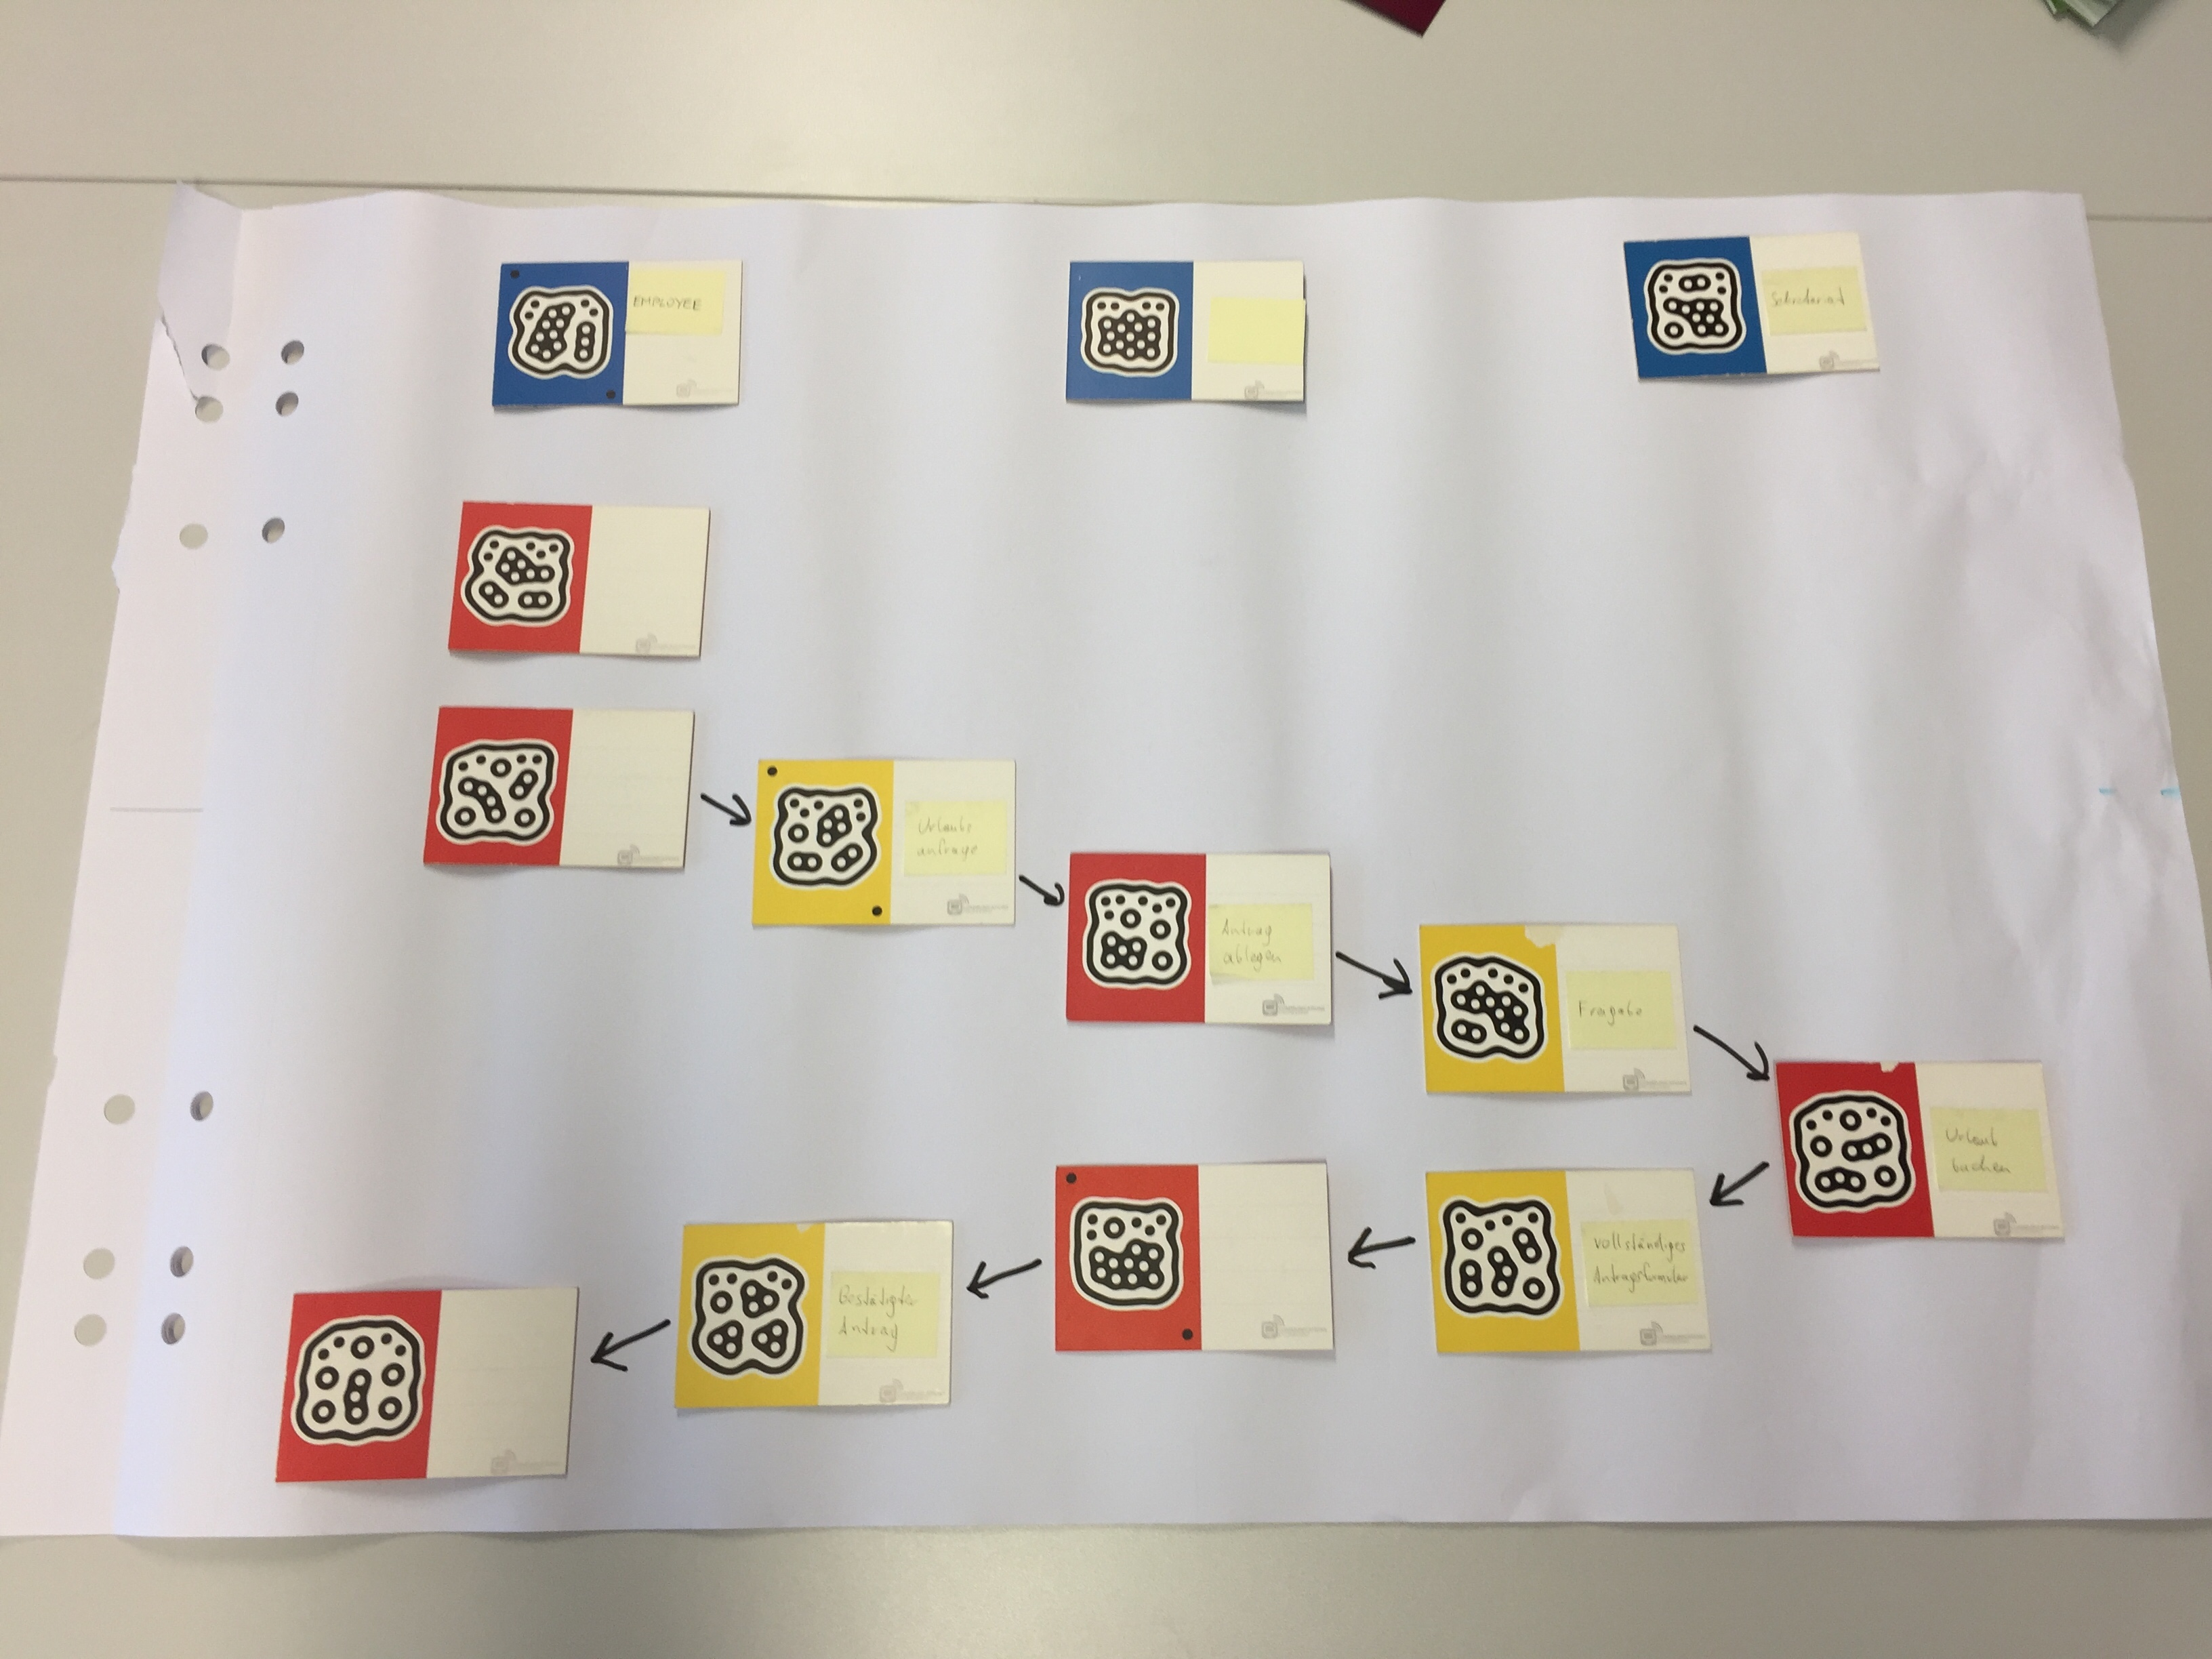
\includegraphics[width=\linewidth]{figures/01.jpg} & Ja & Dieses Beispiel entspricht den Kriterien der Legetechnik. \\
		\midrule
		2 & 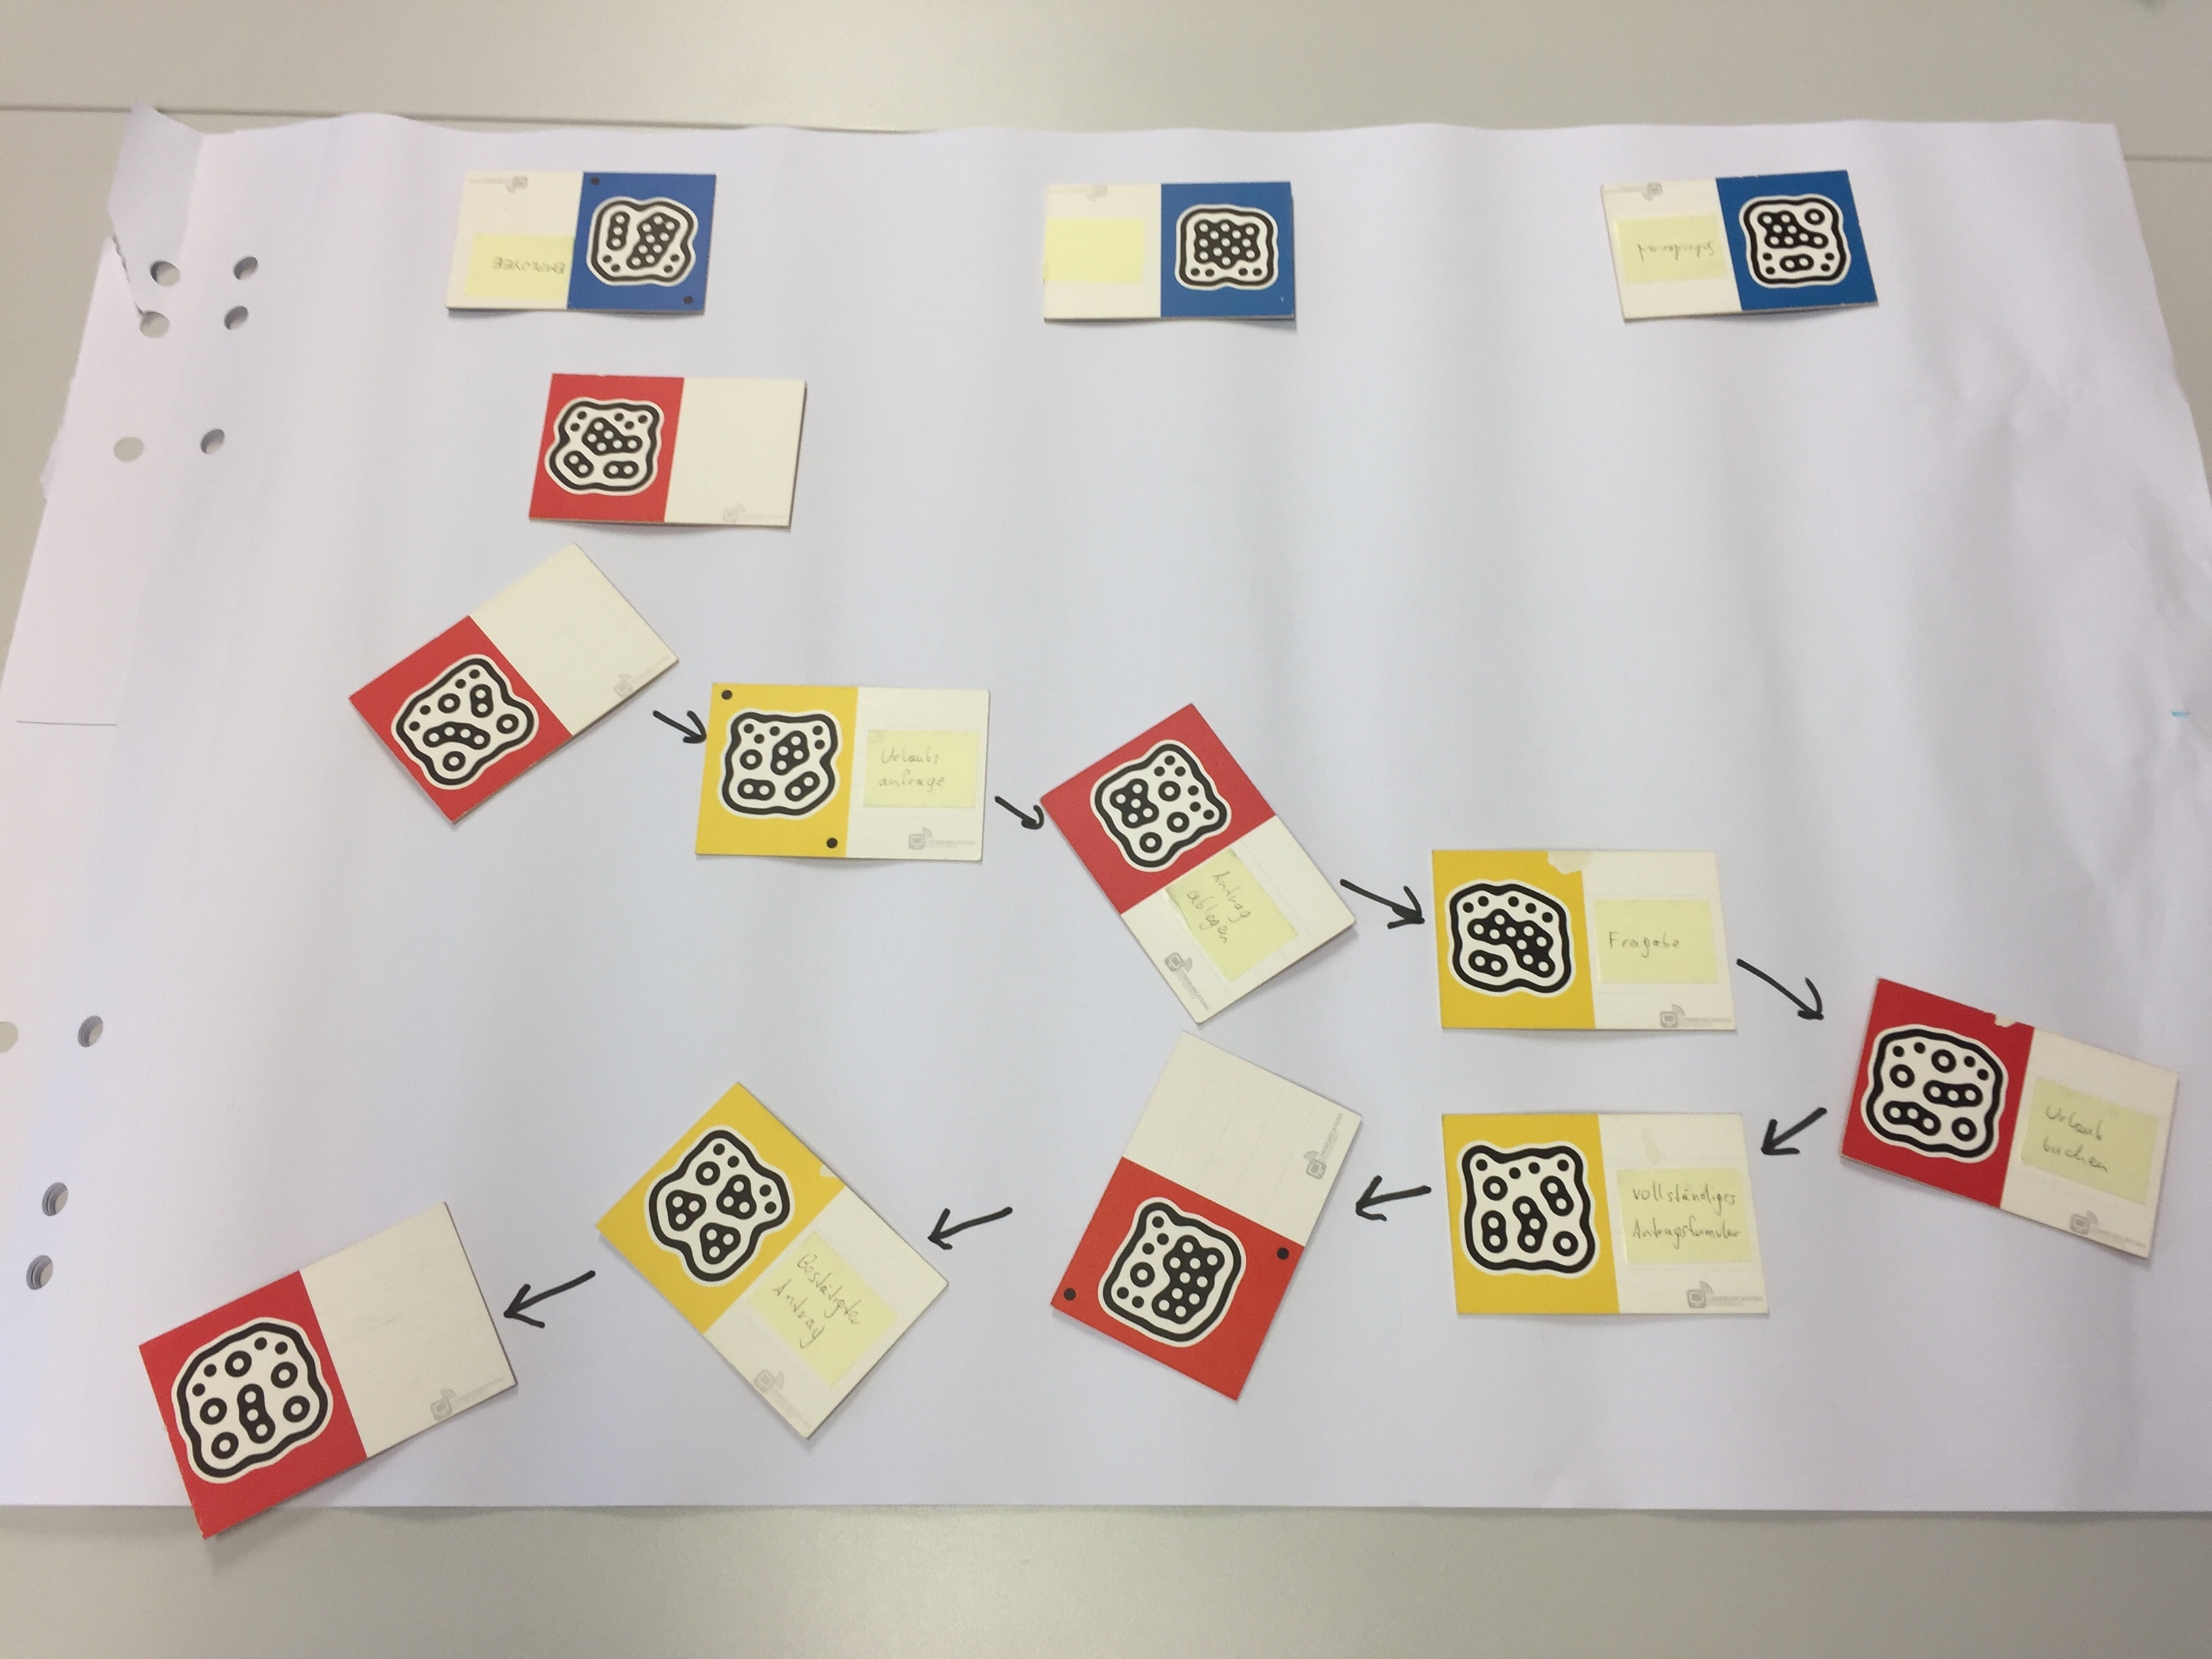
\includegraphics[width=\linewidth]{figures/02.jpg} & Ja & In diesem Beispiel ist ersichtlich, dass die Karten nicht exakt vertikal angeordnet sein müssen, und die Rotation der Karten keinen Einfluss auf das Ergebnis hat. \\
		\midrule
		3 & 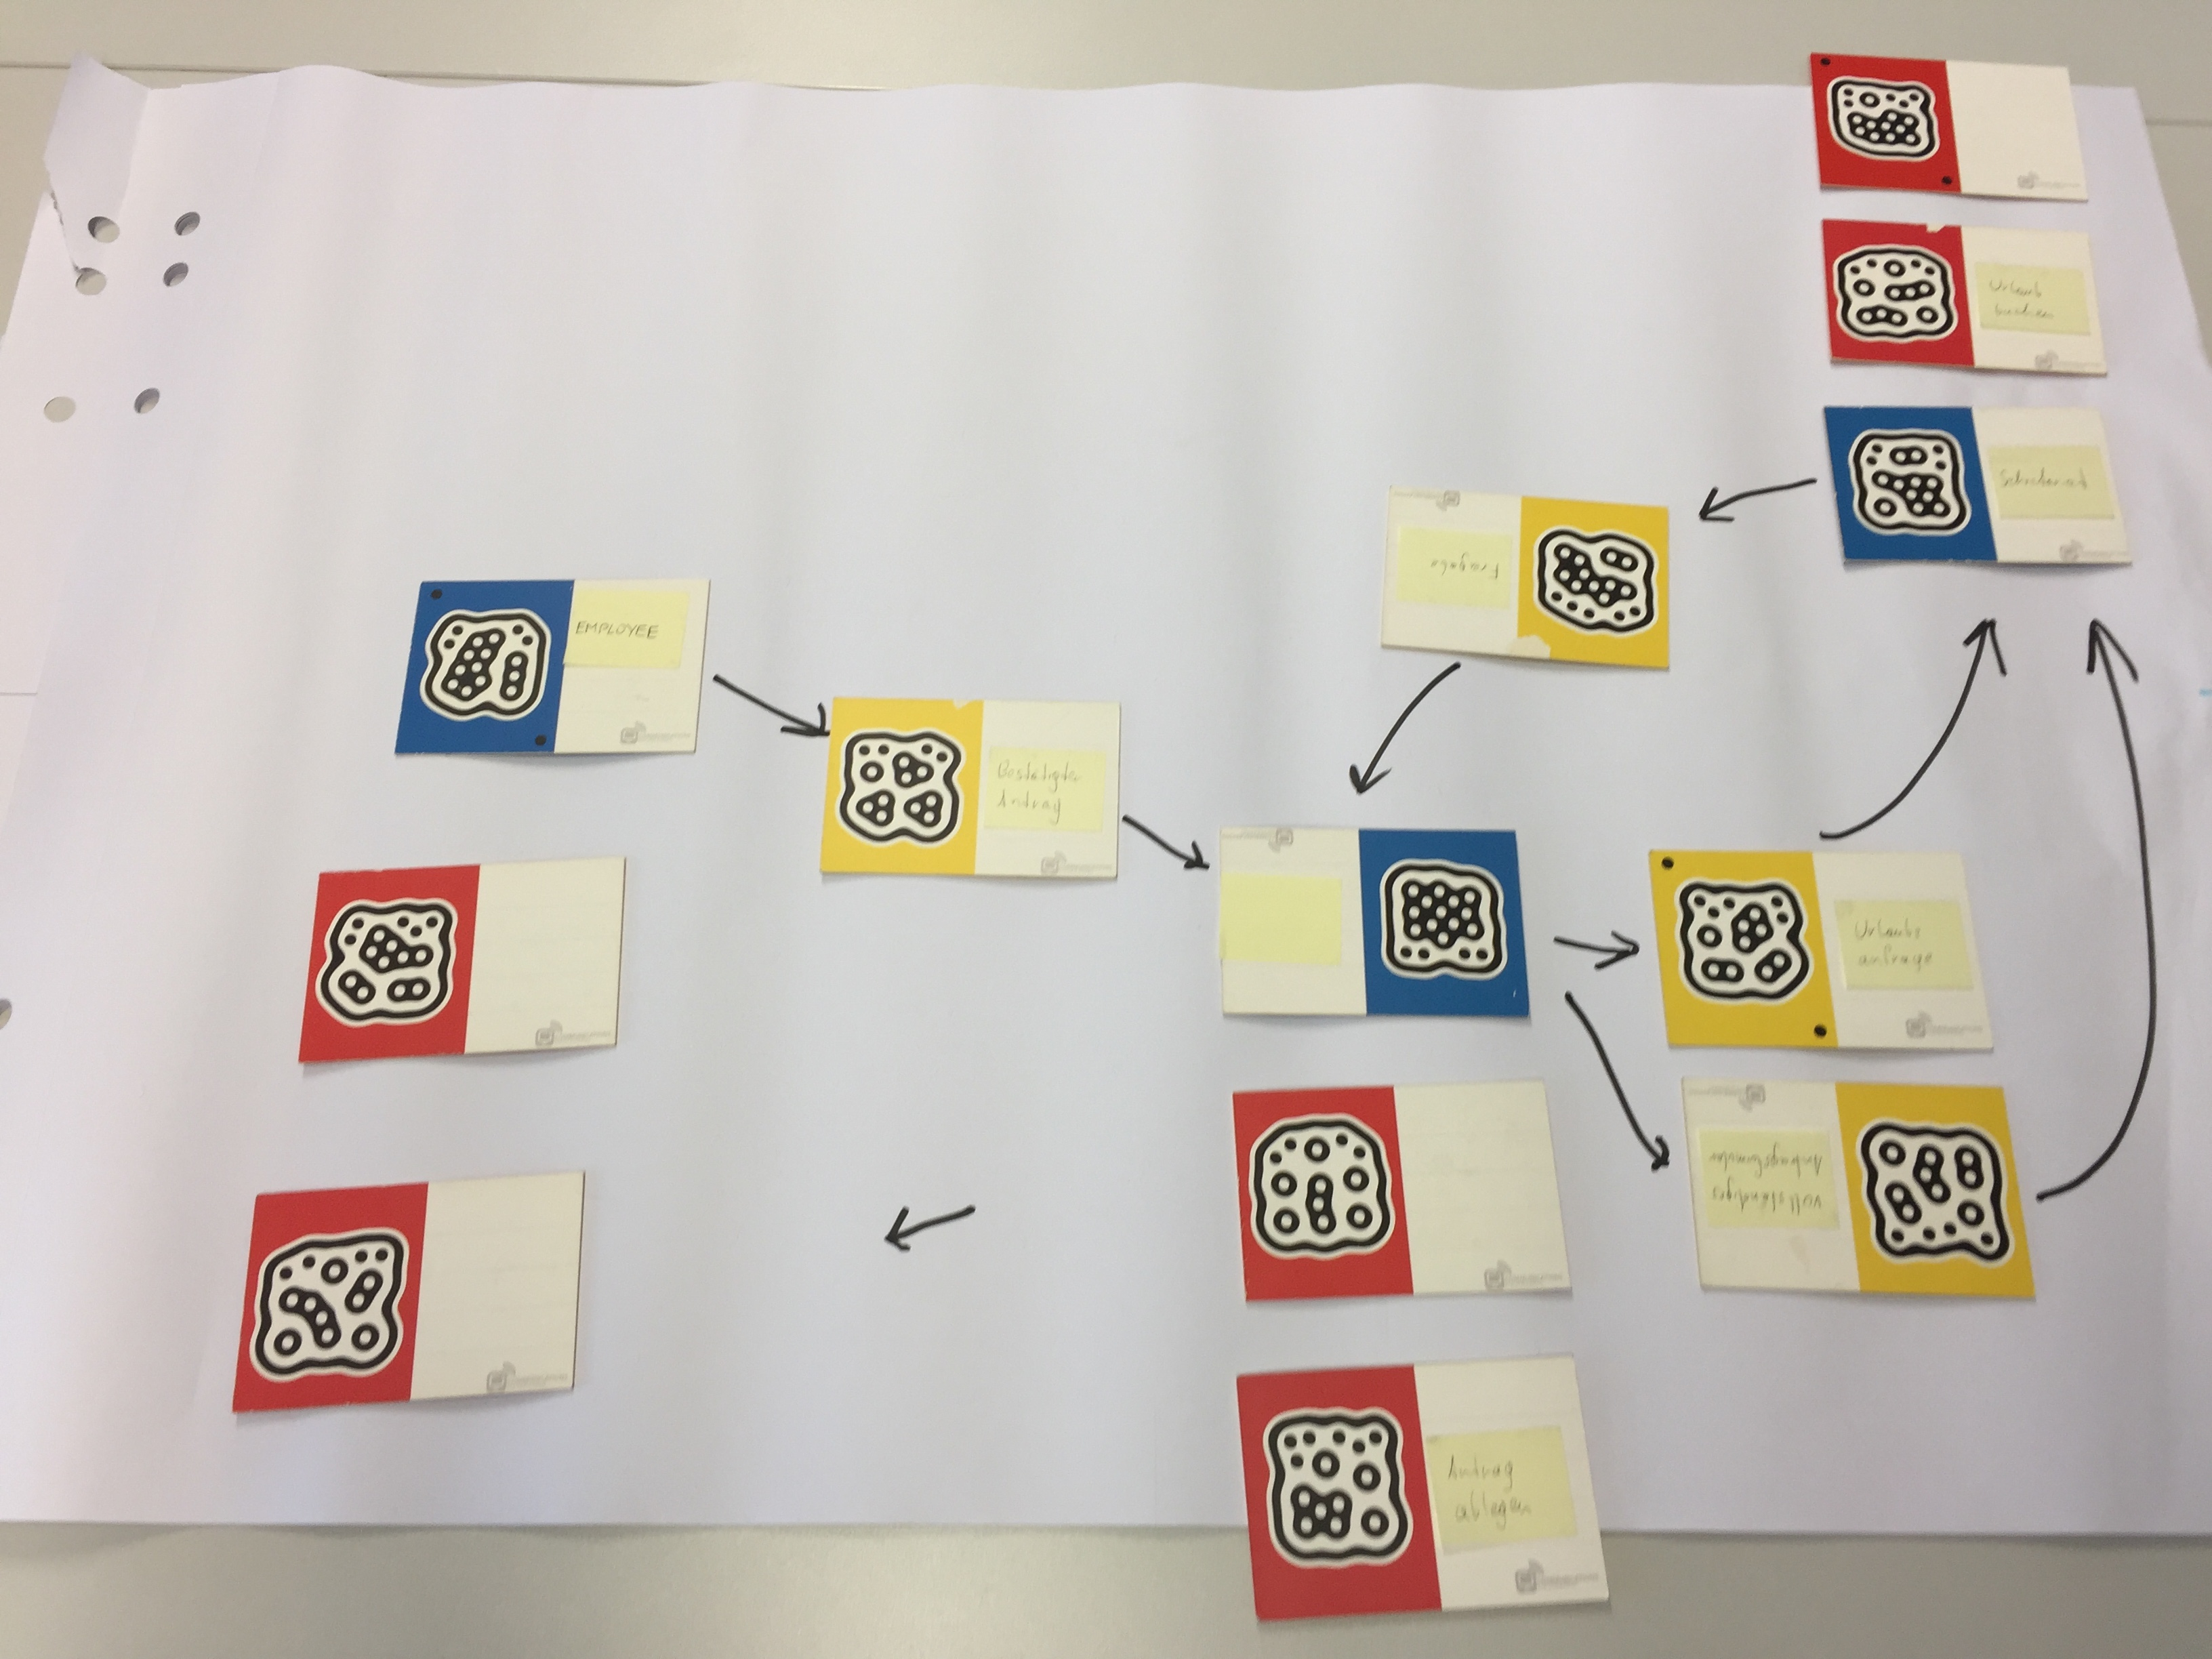
\includegraphics[width=\linewidth]{figures/03.jpg} & Ja & Die Zuordnungen werden richtig erkannt obwohl die Anordnung der Subjekte nicht den Legevorschriften entspricht. \\
		\midrule
		4 & 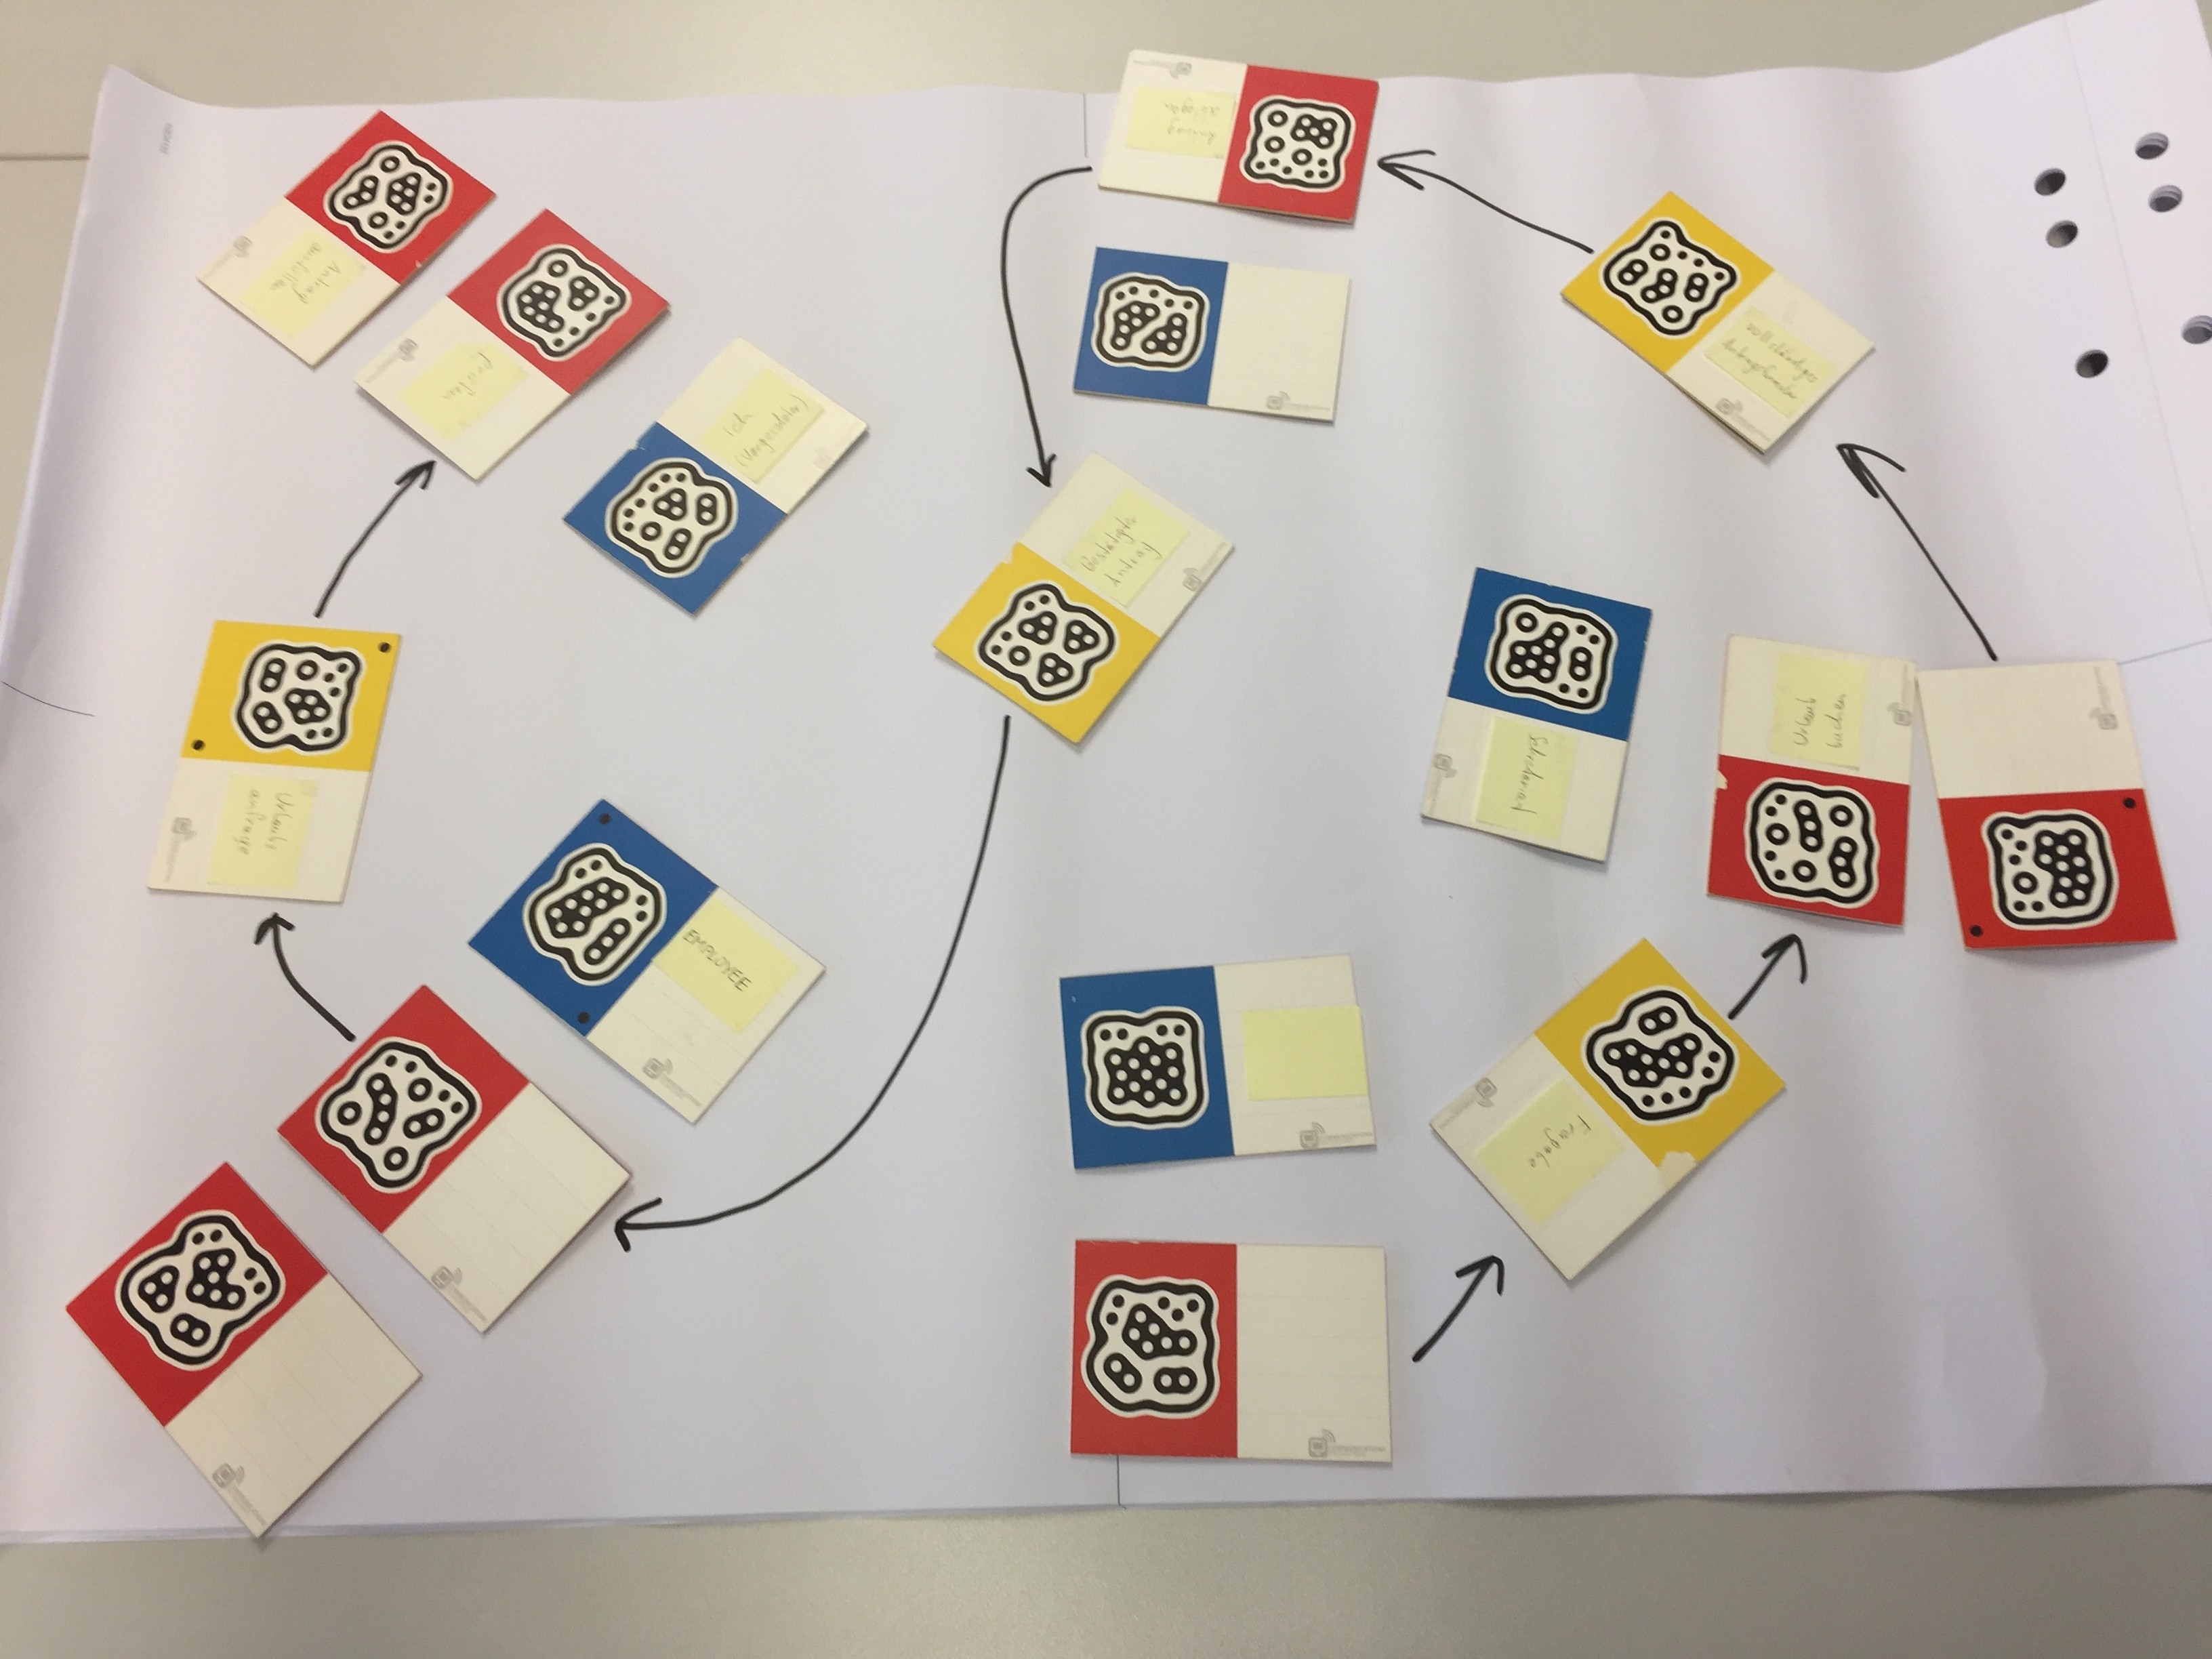
\includegraphics[width=\linewidth]{figures/04.jpg} & Ja & Dieses Beispiel ist dem Anschein nach als Sternlayout gelegt. Dennoch wird das Muster erkannt, da die Aufgaben jedes Subjekts in Linie gelegt sind. \\
		\midrule
		5 & 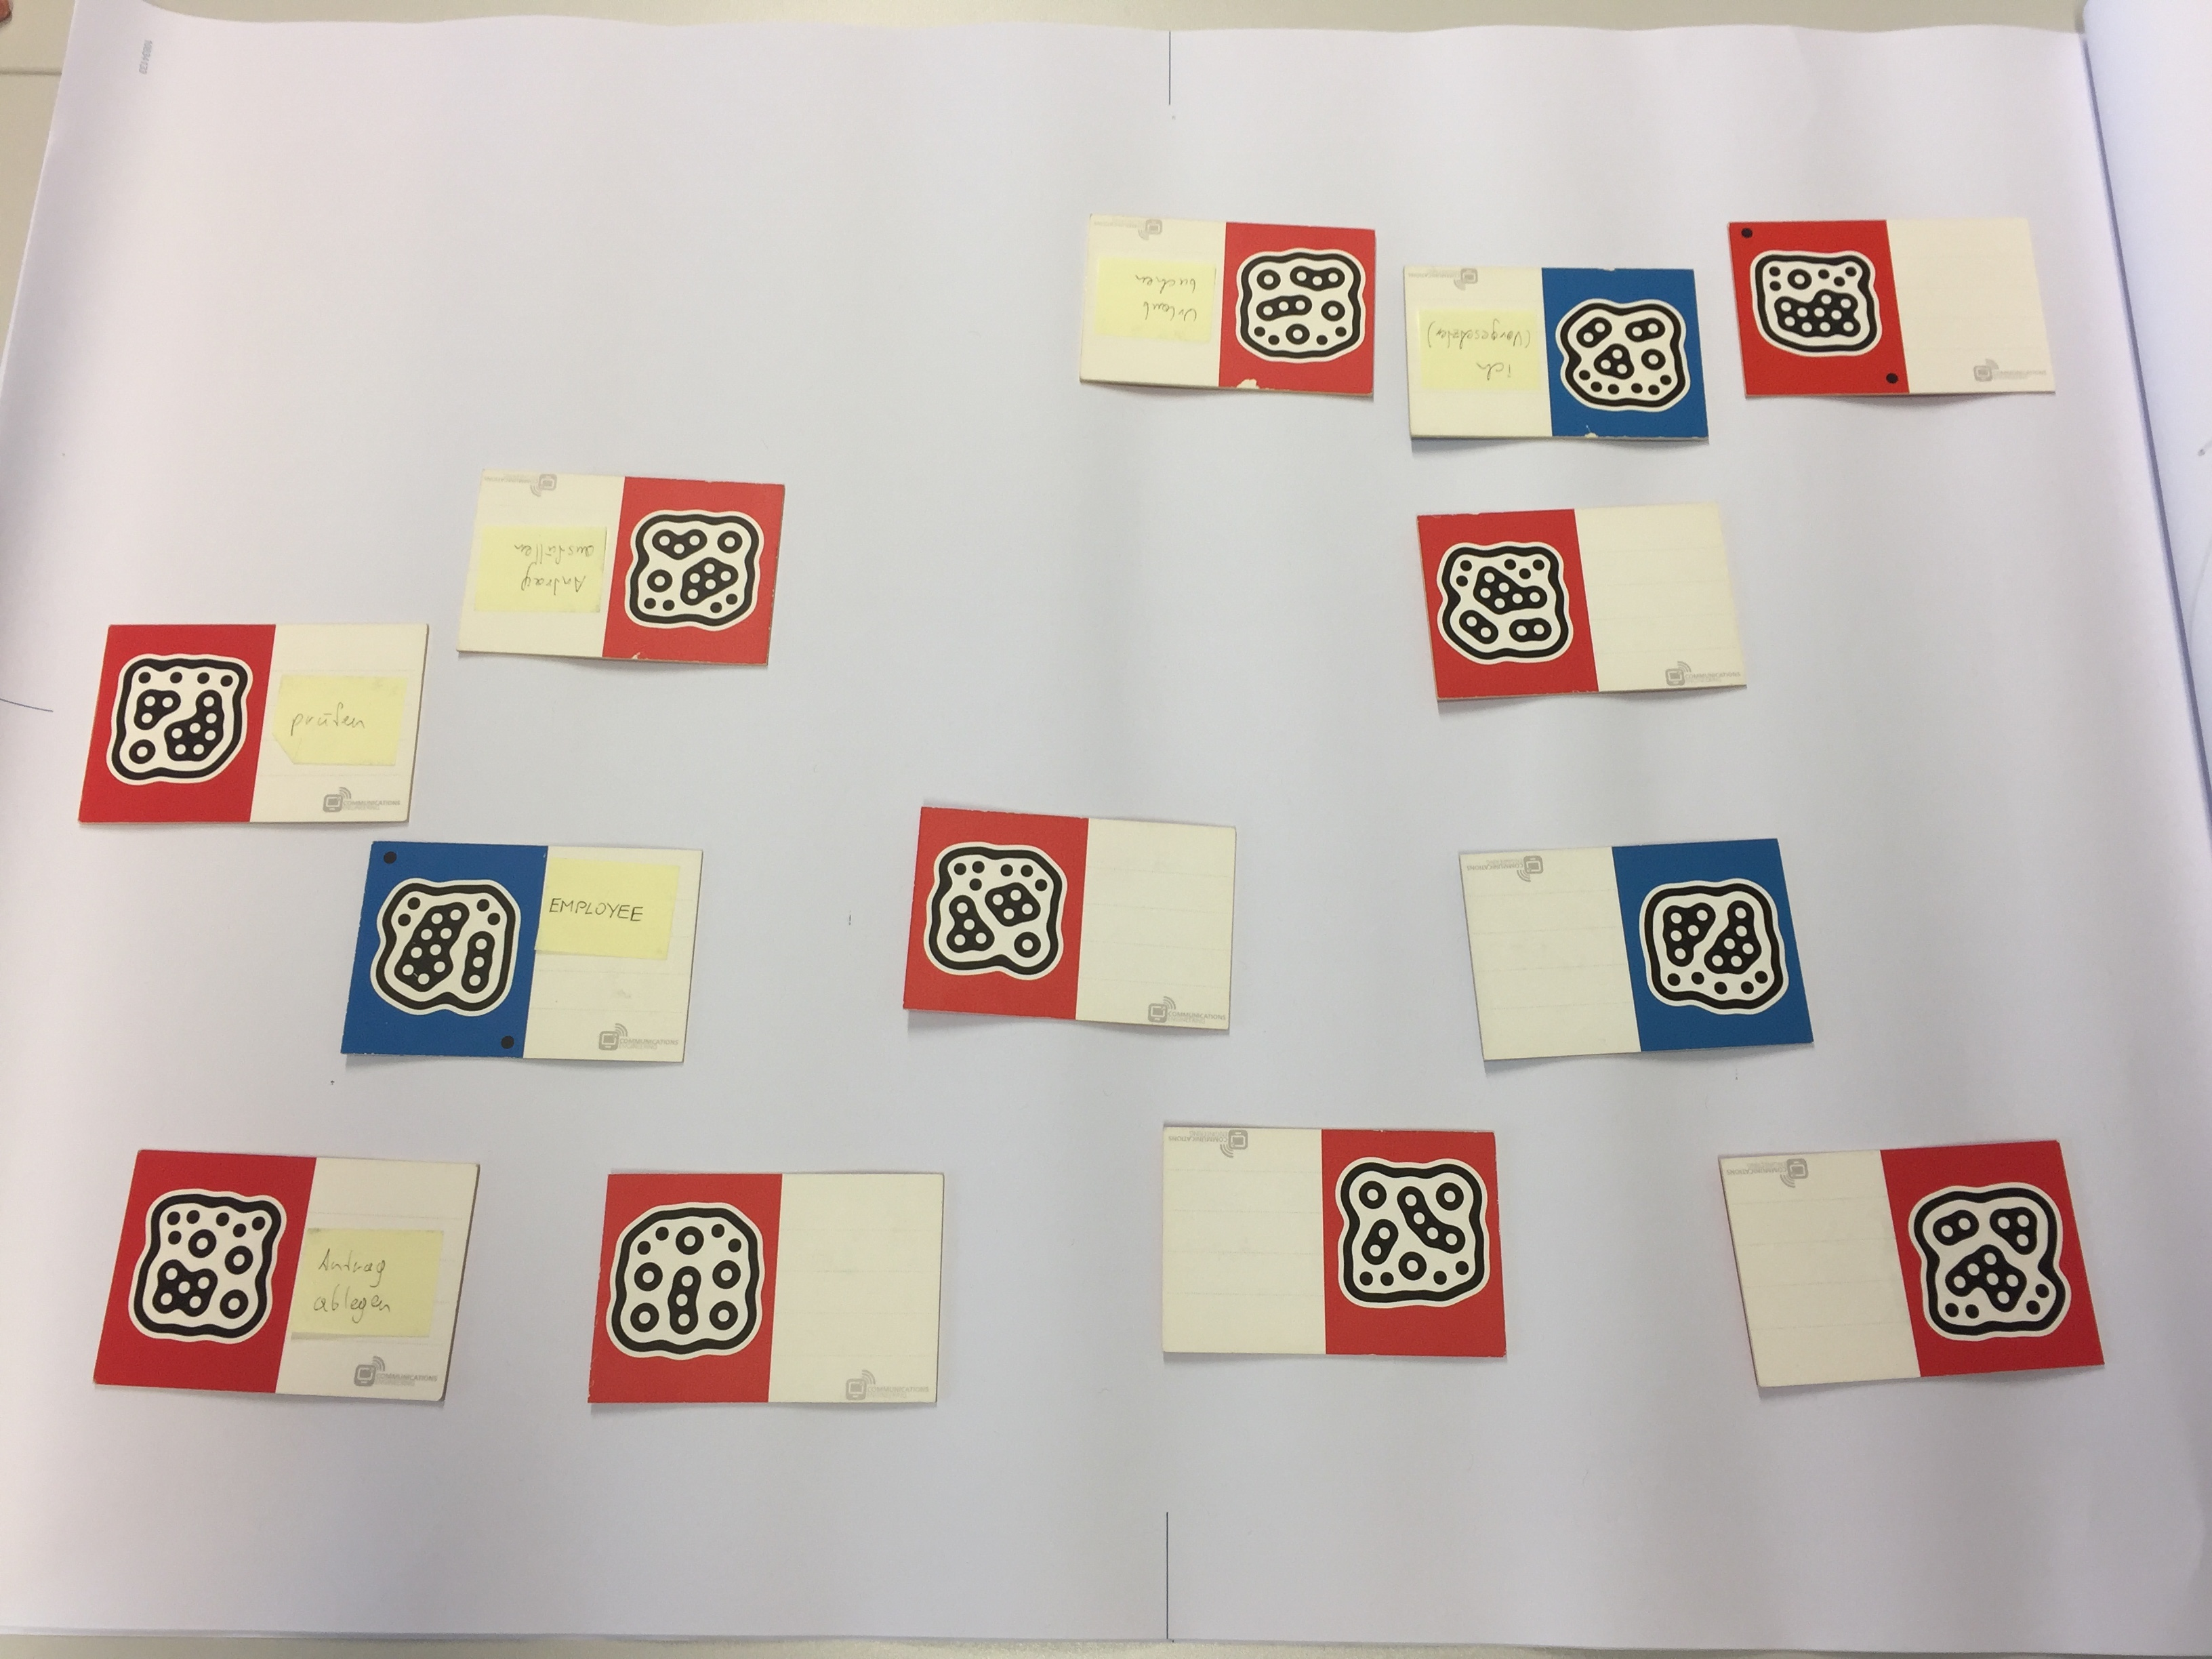
\includegraphics[width=\linewidth]{figures/05.jpg} & Ja & Der Testfall wird als Sternlayout erkannt. \\
		\midrule
		6 & 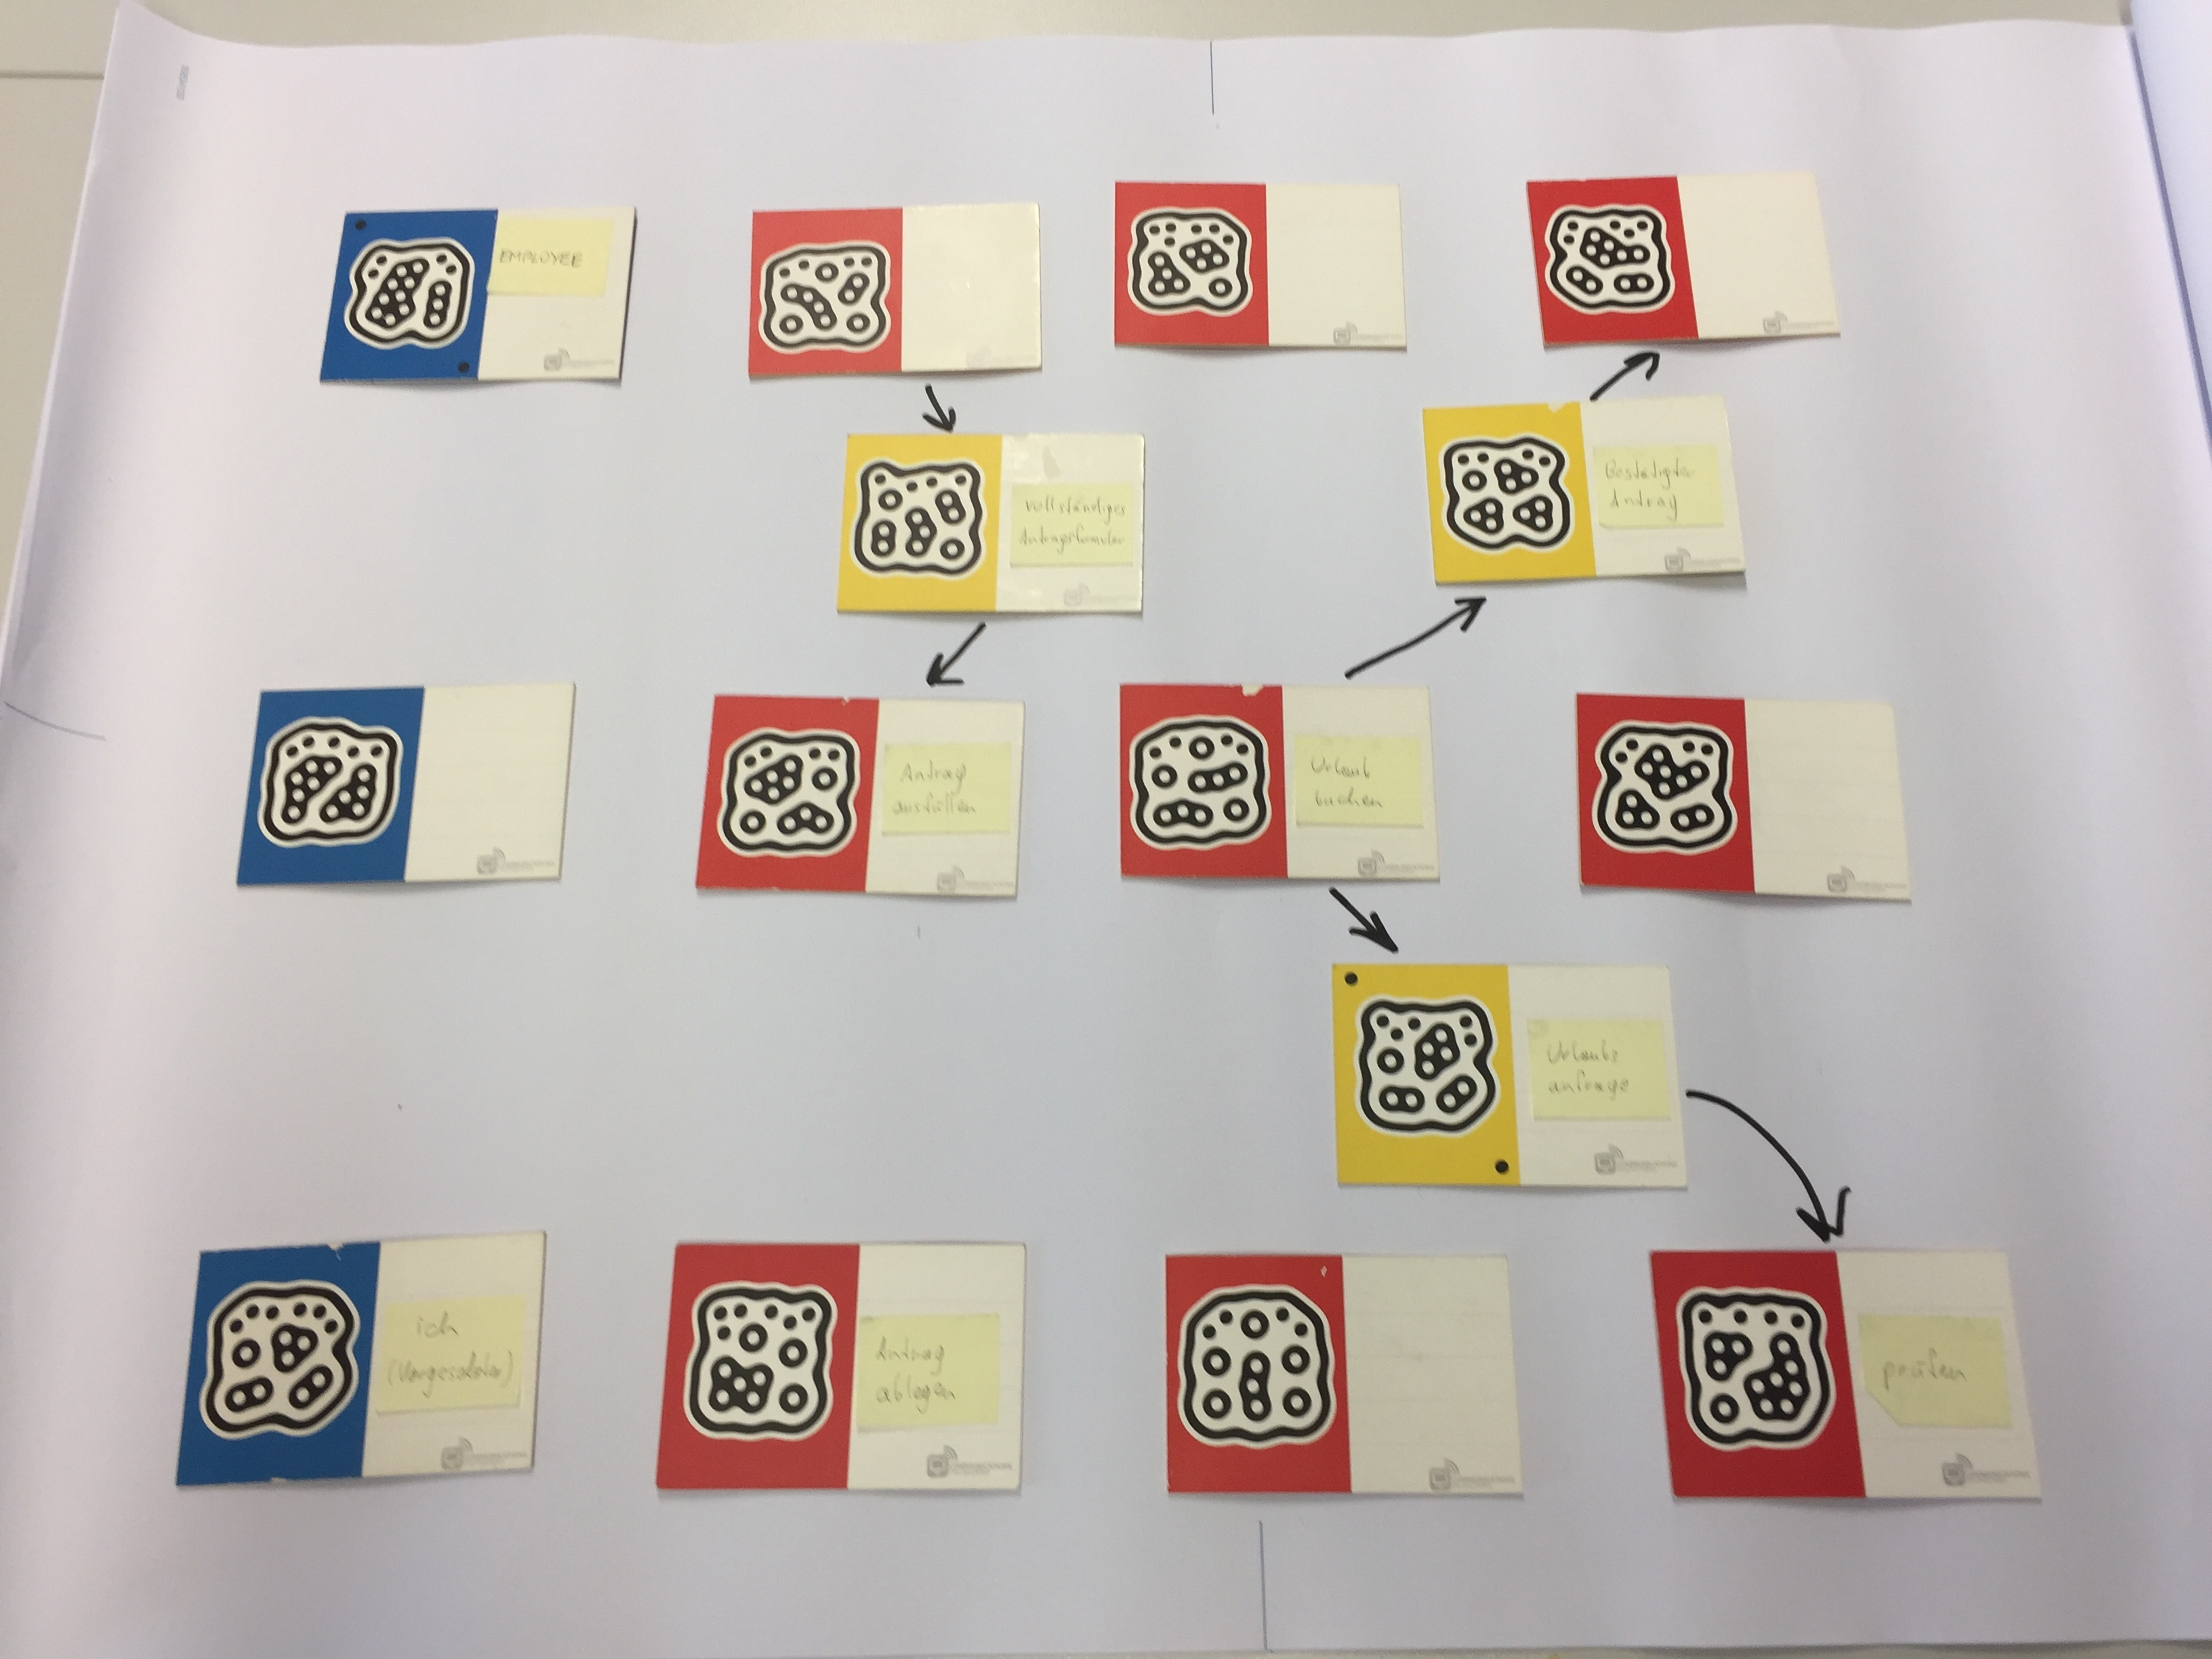
\includegraphics[width=\linewidth]{figures/06.jpg} & Ja & Der Testfall wird richtig erkannt. Die horizontale Ausrichtung der Aufgaben wirkt sich nicht auf das Ergebnis des Algorithmus aus. \\
		\midrule
		7 & 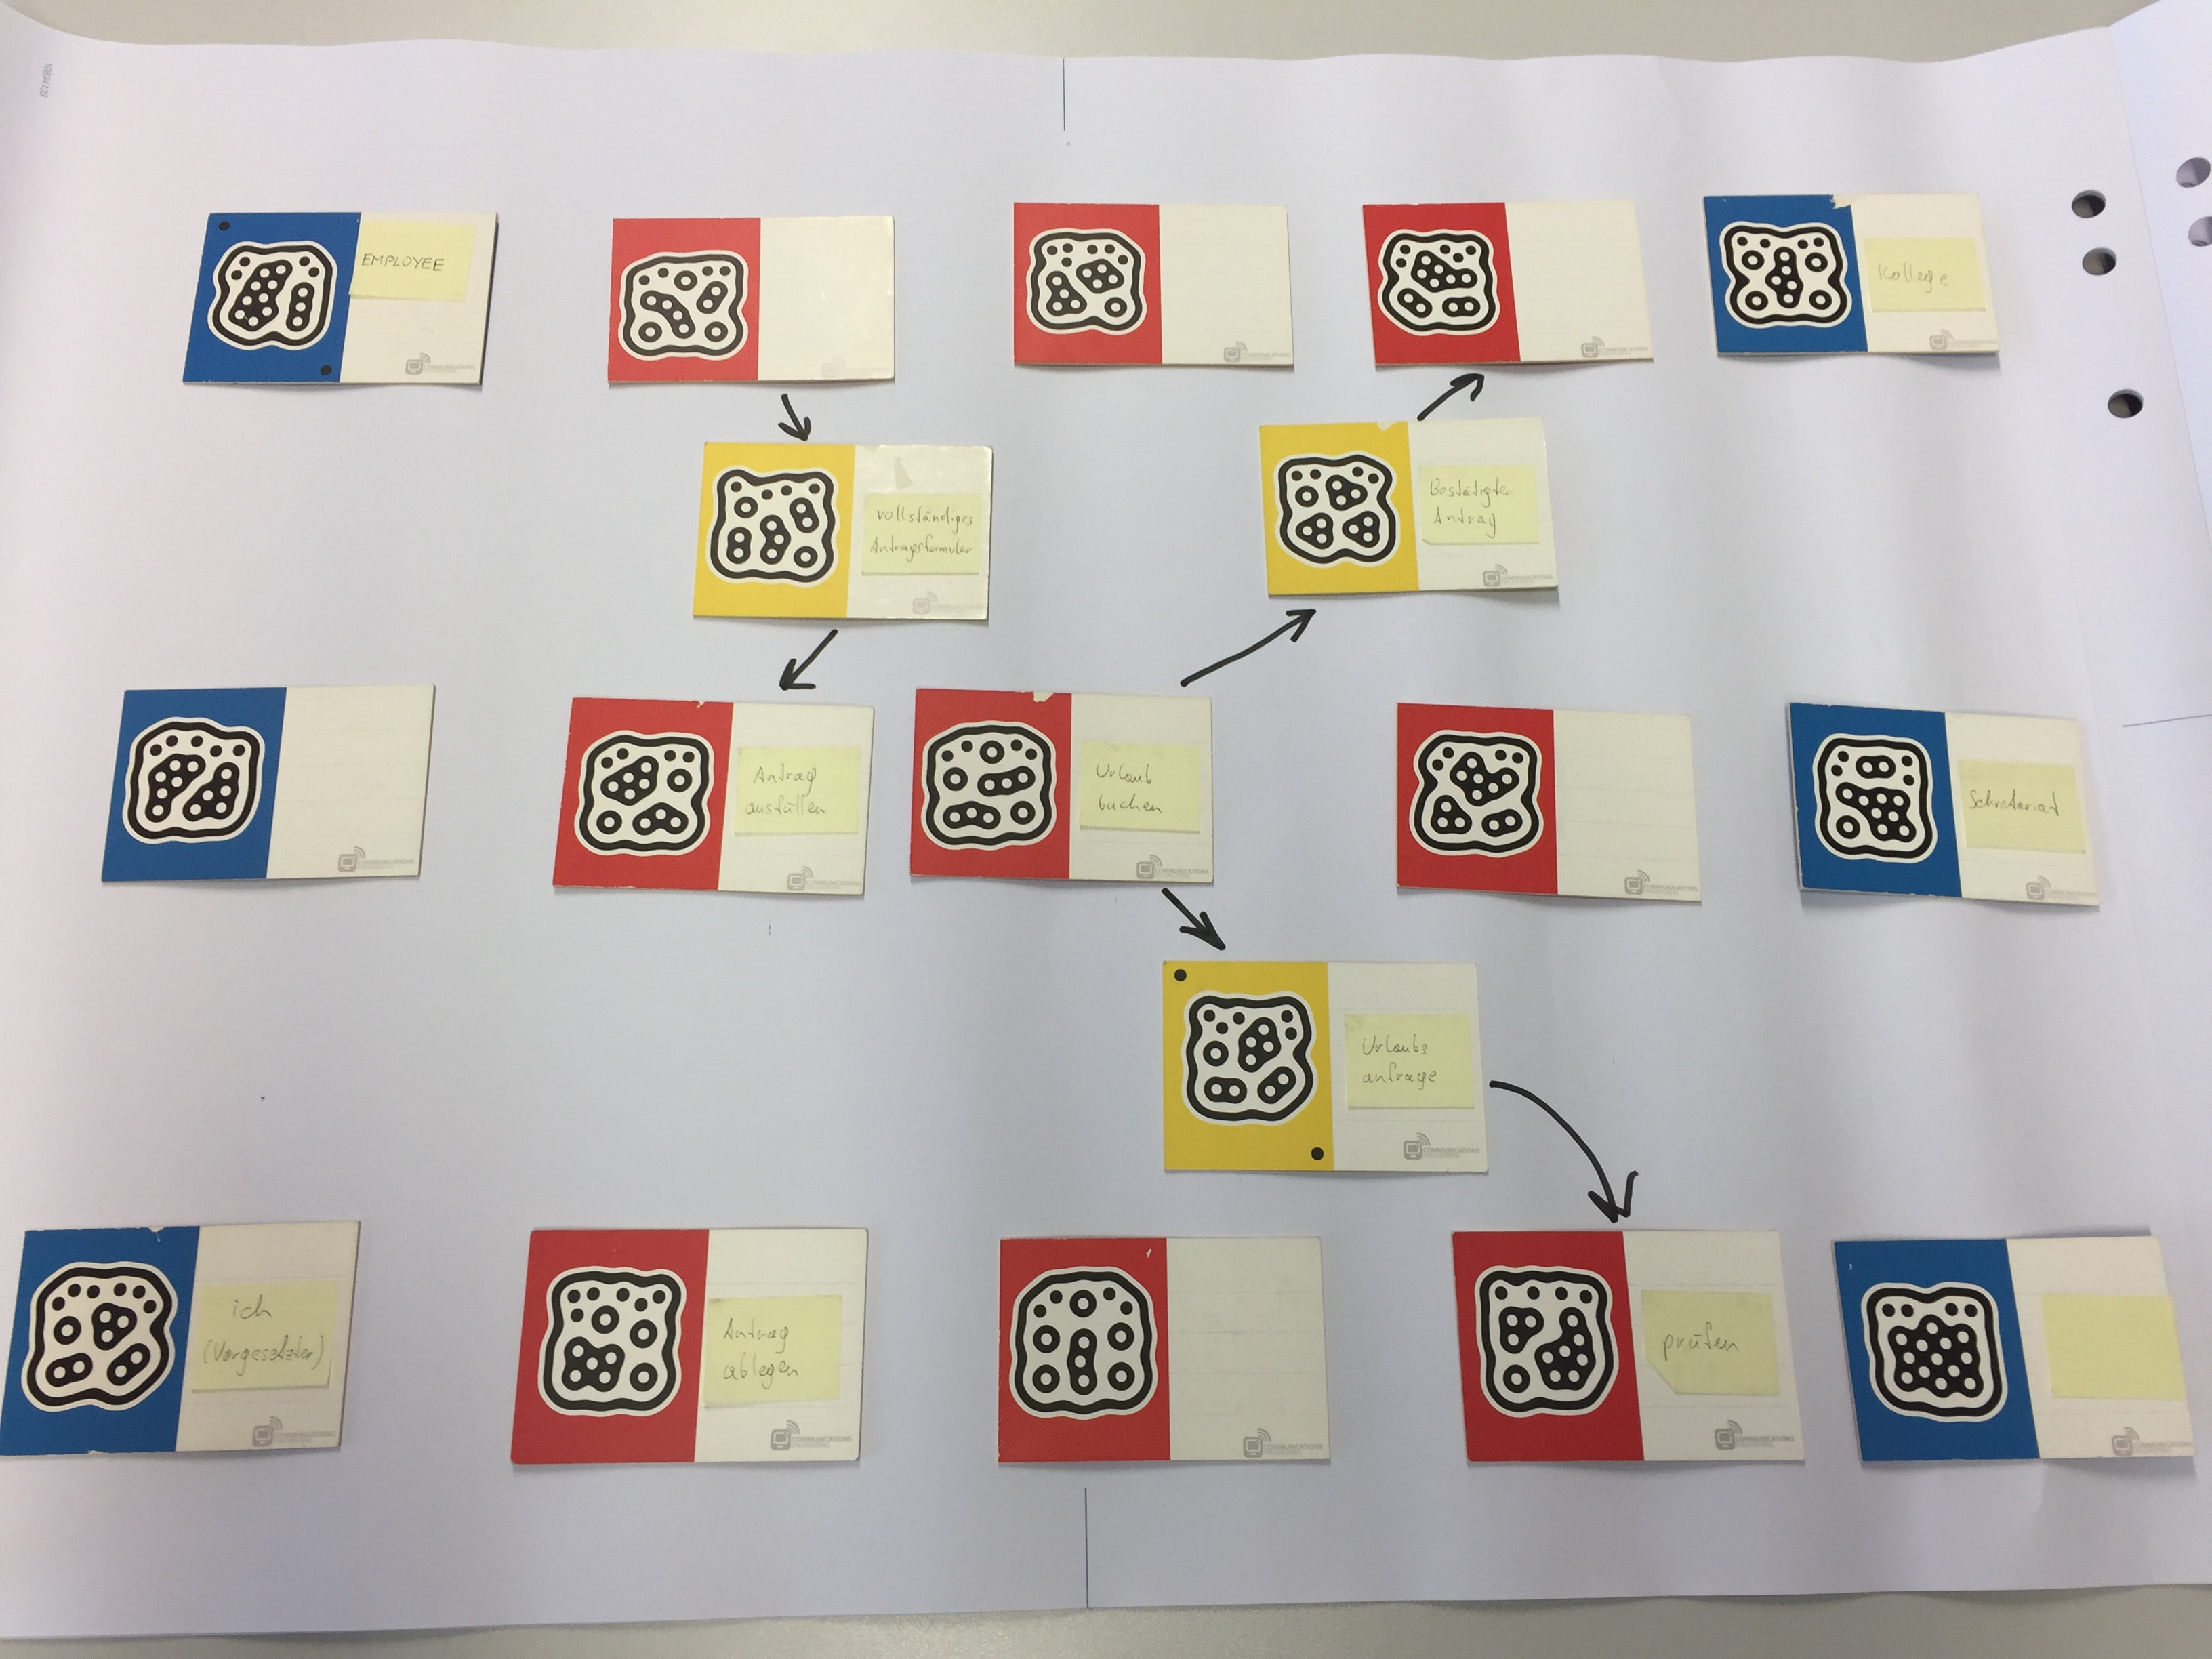
\includegraphics[width=\linewidth]{figures/07.jpg} & Ja & Der Testfall wird erkannt. Dabei werden die mittleren Aufgabenkarten korrekt über den minimalen Abstand zum Subjekt zugeordnet. \\
		\midrule
		8 & 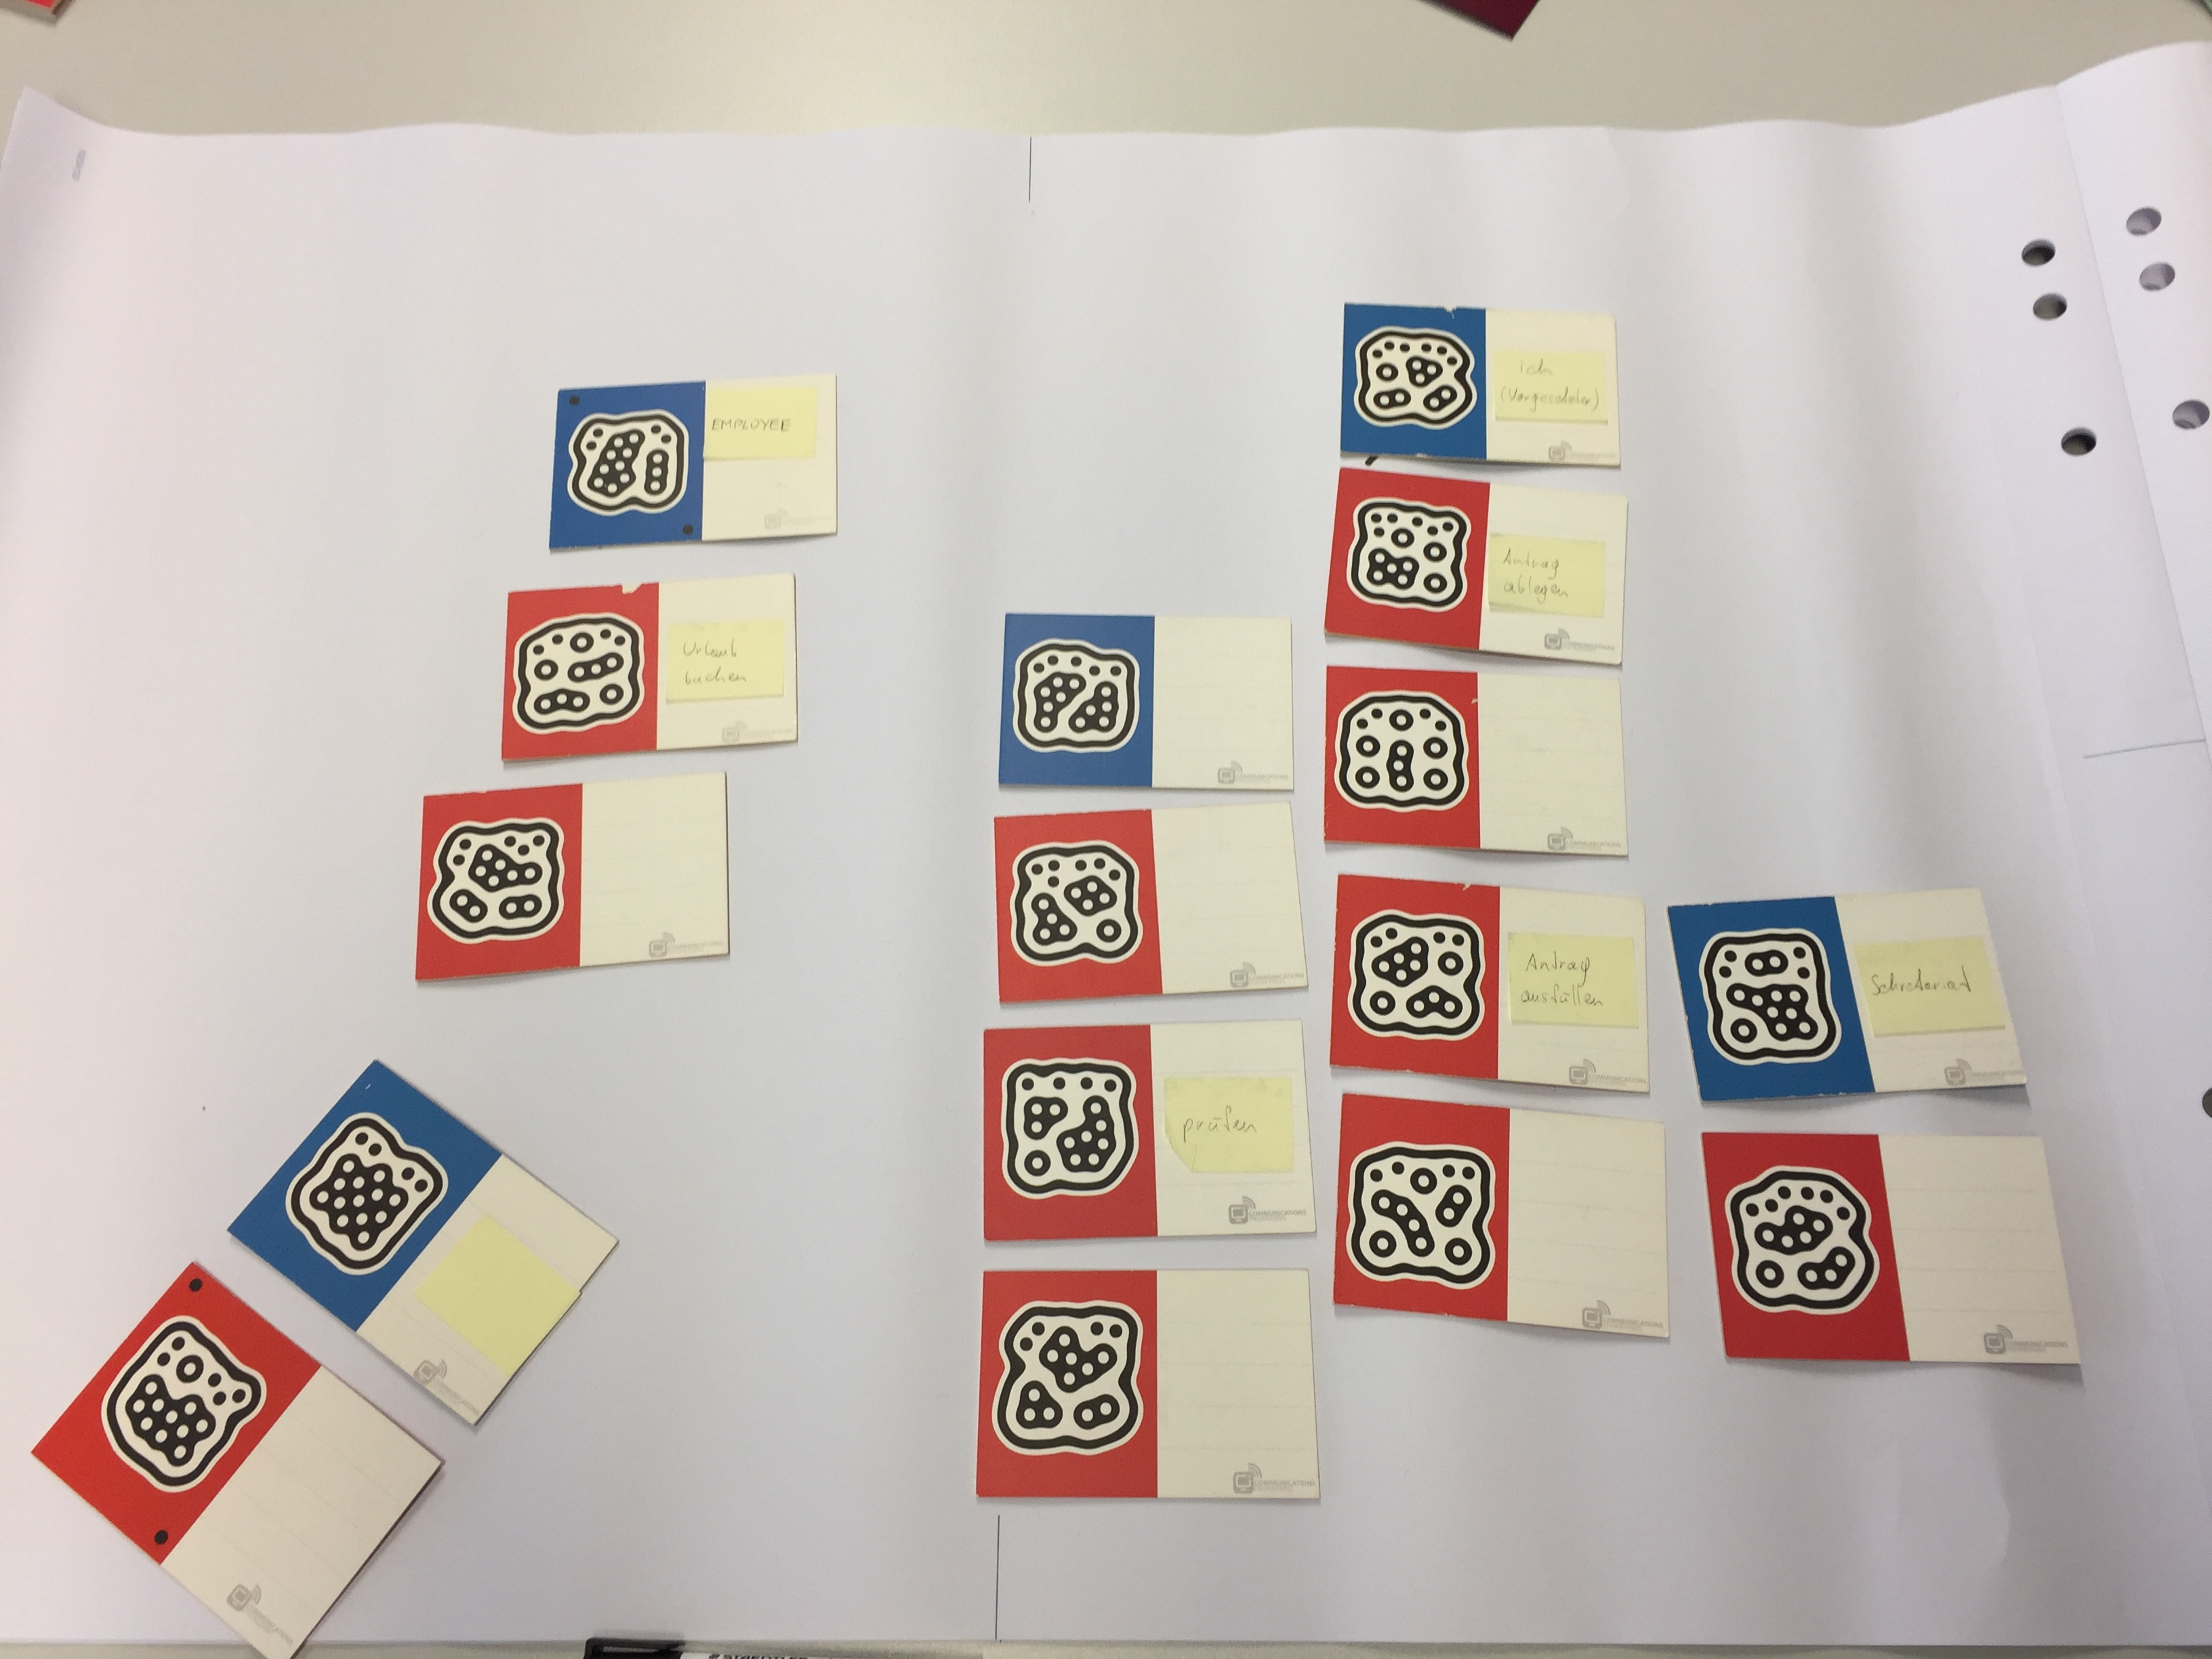
\includegraphics[width=\linewidth]{figures/08.jpg} & Ja & In diesem Beispiel wird die Aufgabe im linken unteren Eck korrekt zugeordnet, da der Vektor vom oberen linken Subjekt zur Aufgabe ein Subjekt schneidet.  \\
		\midrule
		9 & 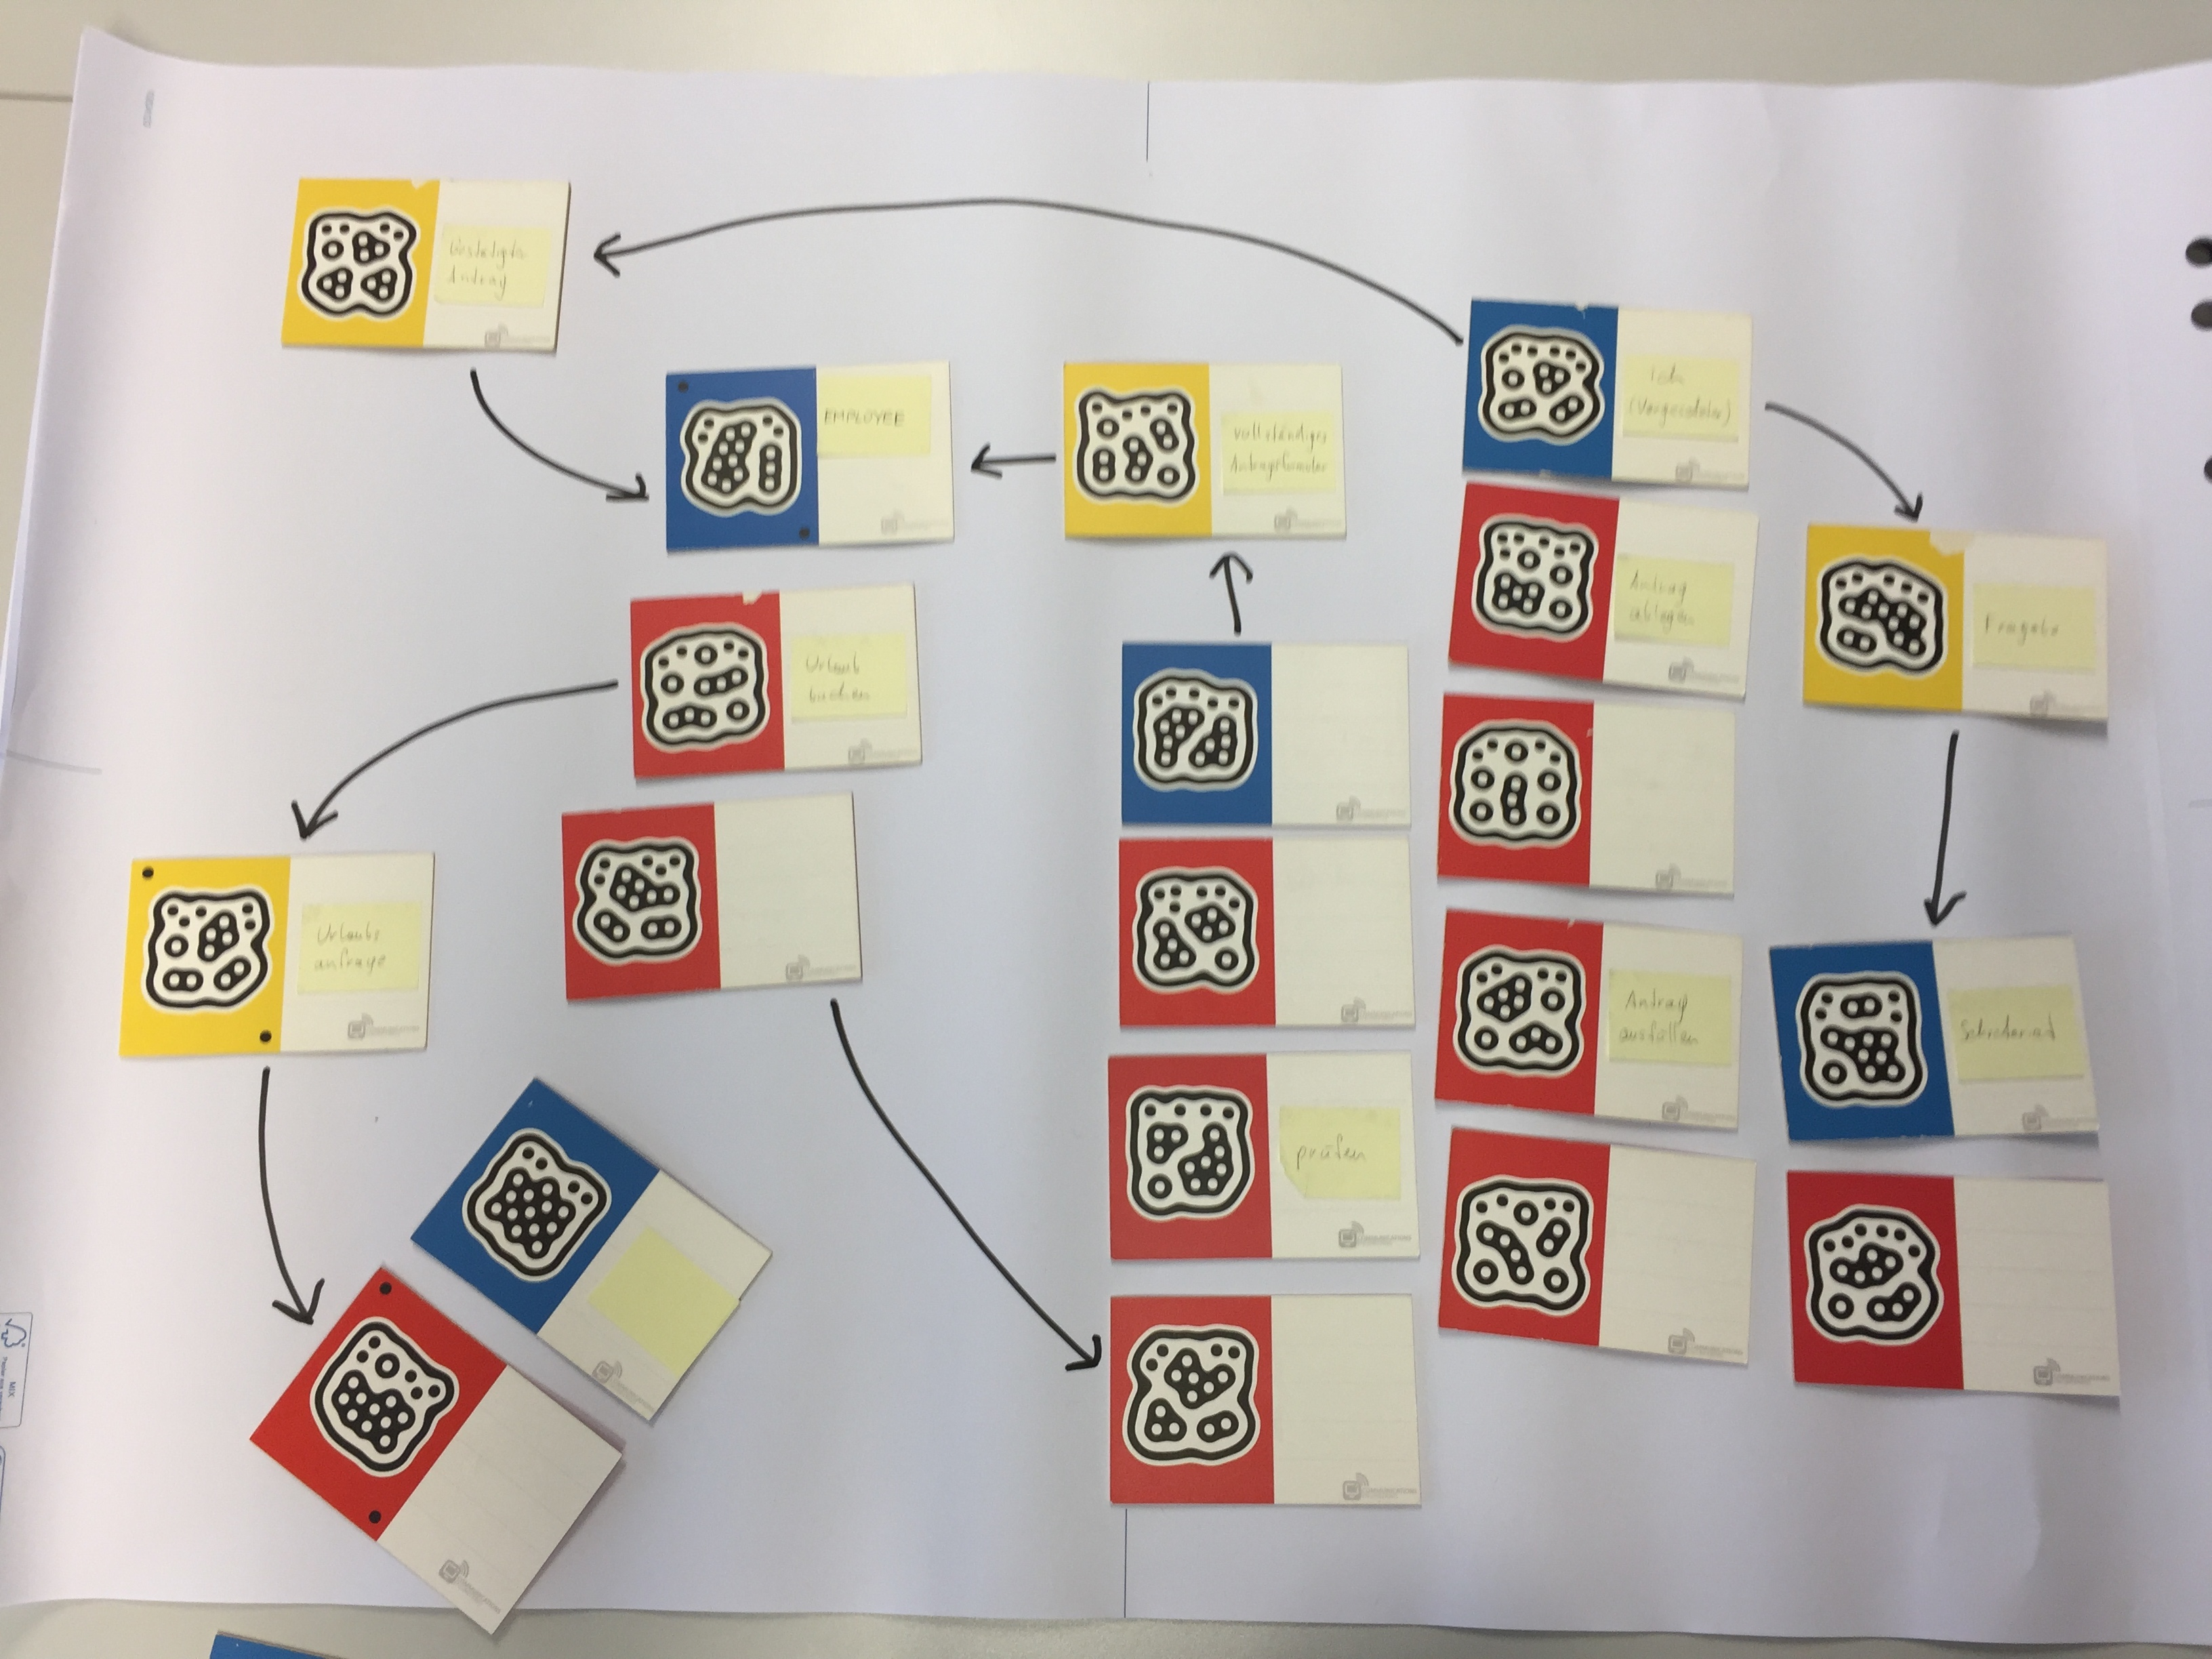
\includegraphics[width=\linewidth]{figures/09.jpg} & Ja & Entspricht in Bezug auf den Algorithmus Testfall 8. \\
		\midrule
		10 & 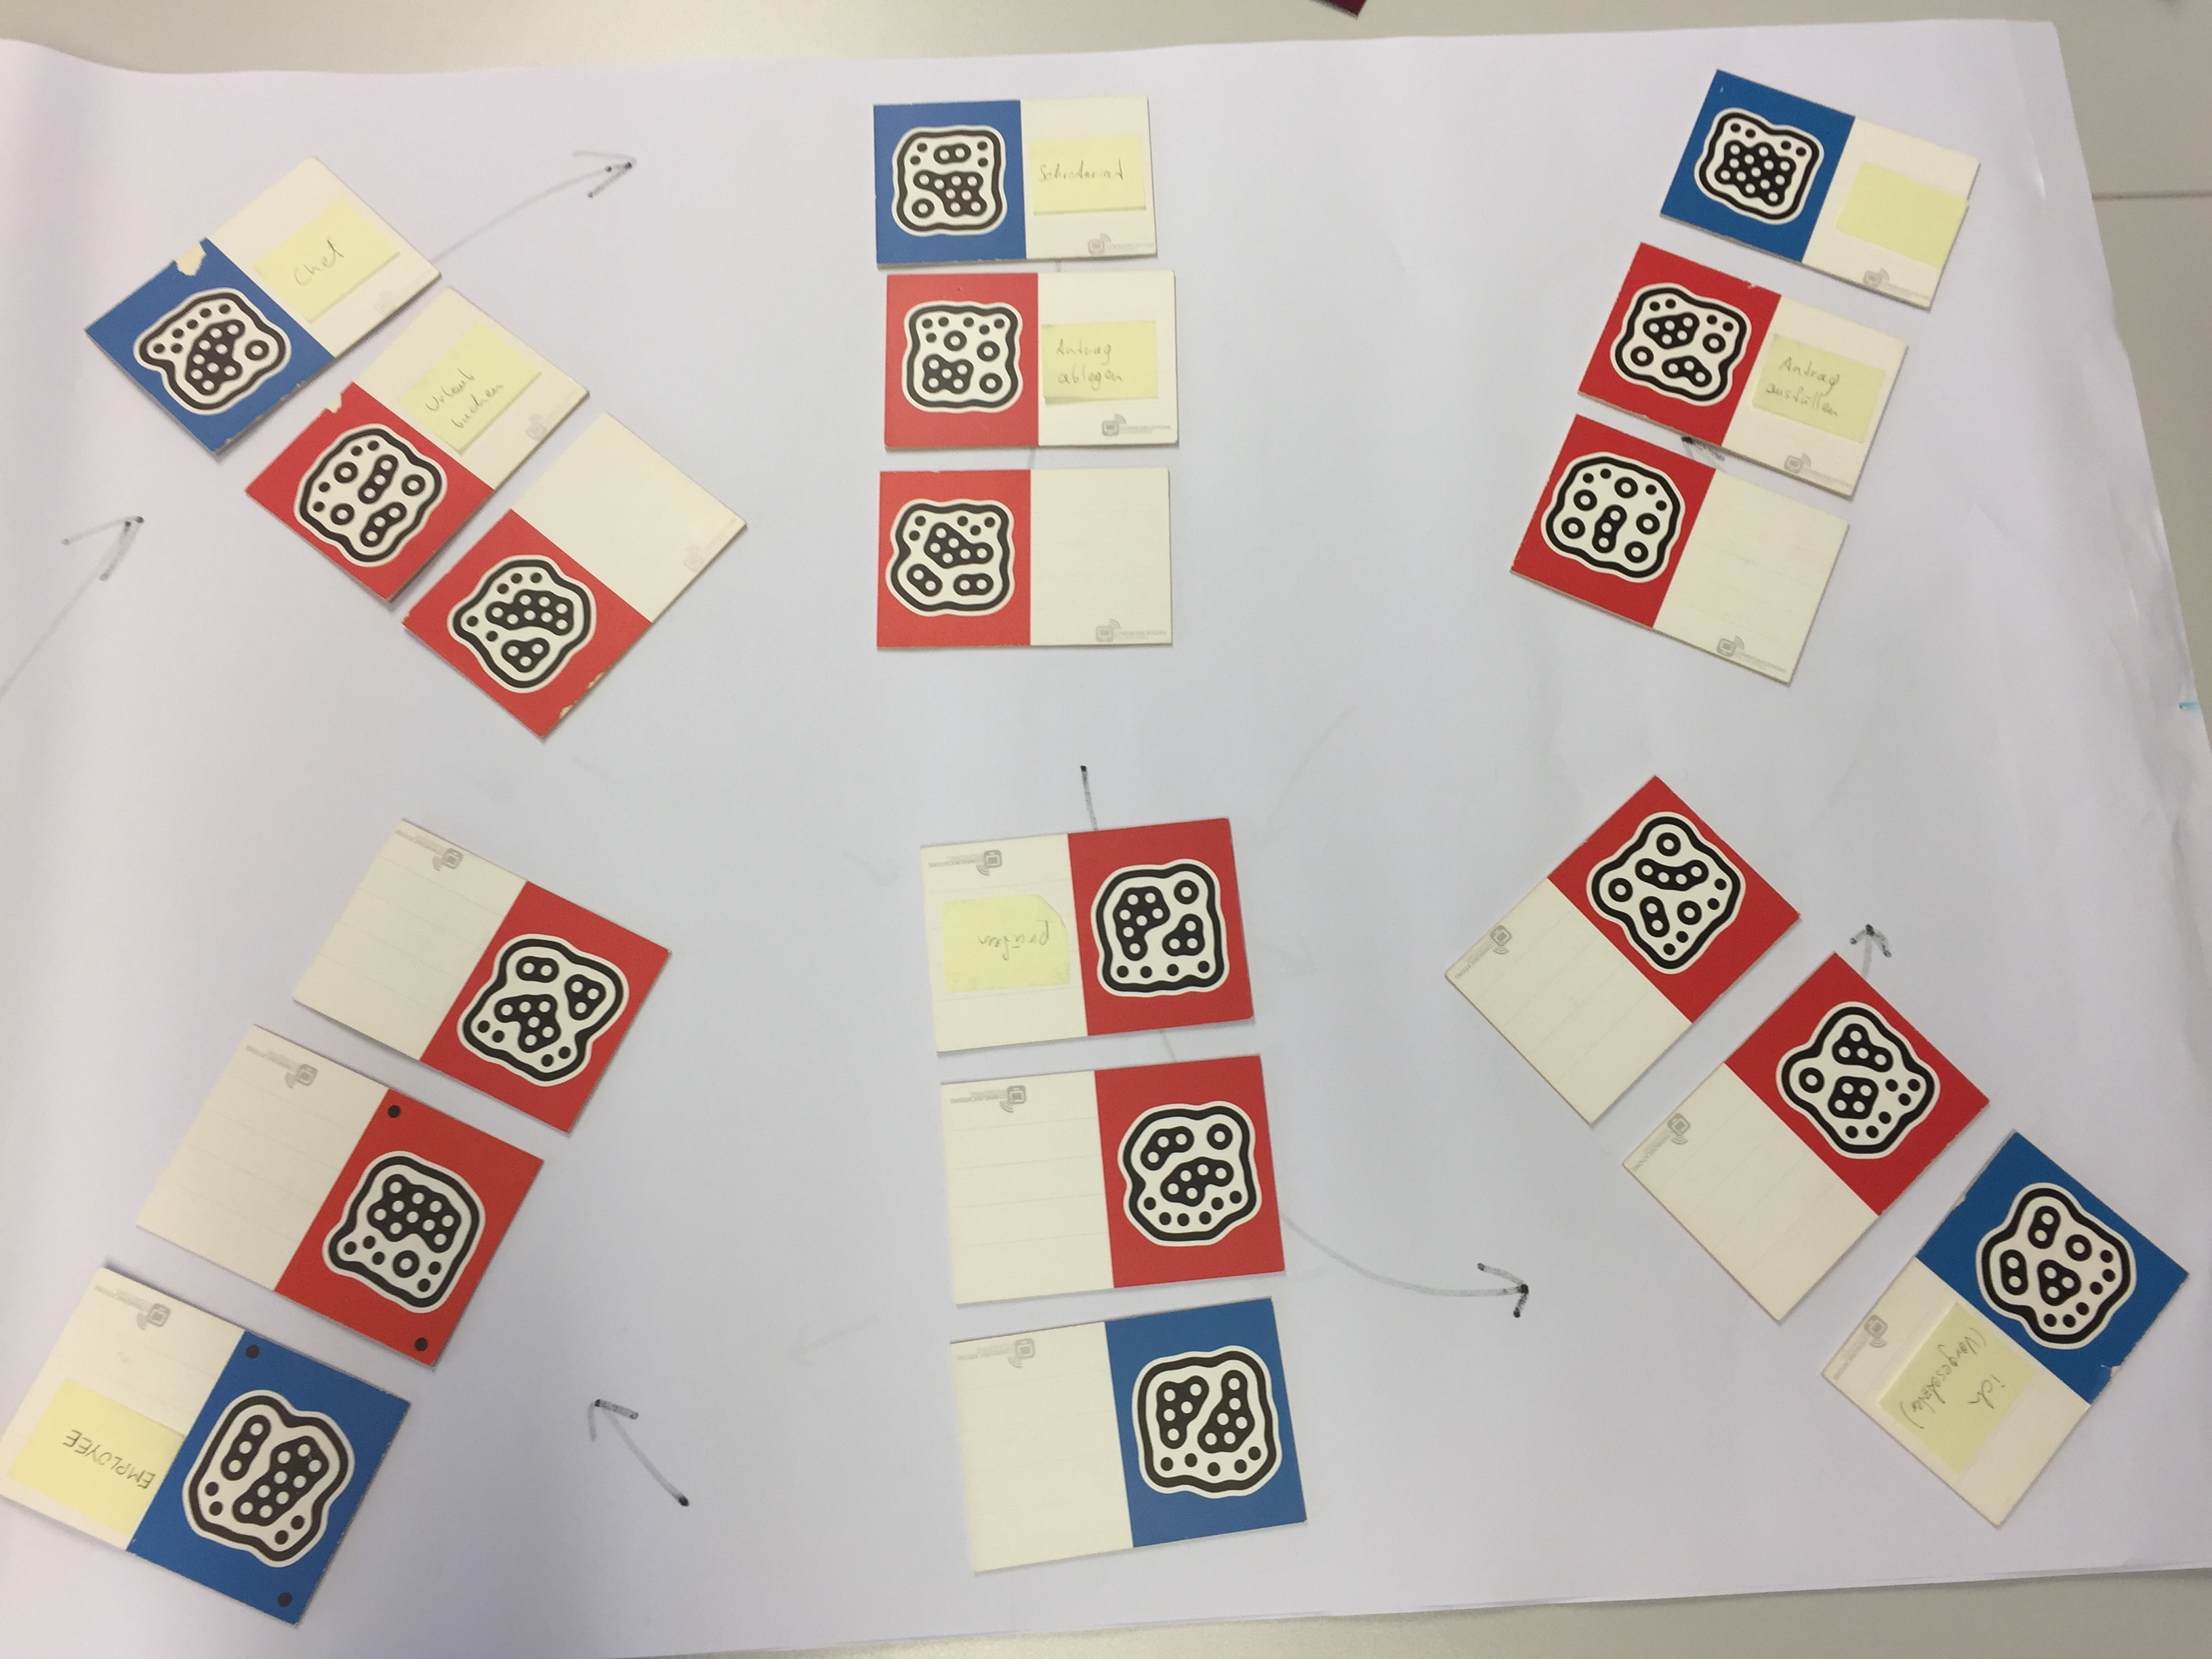
\includegraphics[width=\linewidth]{figures/10.jpg} & Ja & Dieses Beispiel ist scheinbar ein Sternlayout, wird aber korrekt als Linienlayout erkannt. In diesem Fall wird besonders die Funktionalität der Verifizierung geprüft. \\
		\midrule
		11 & 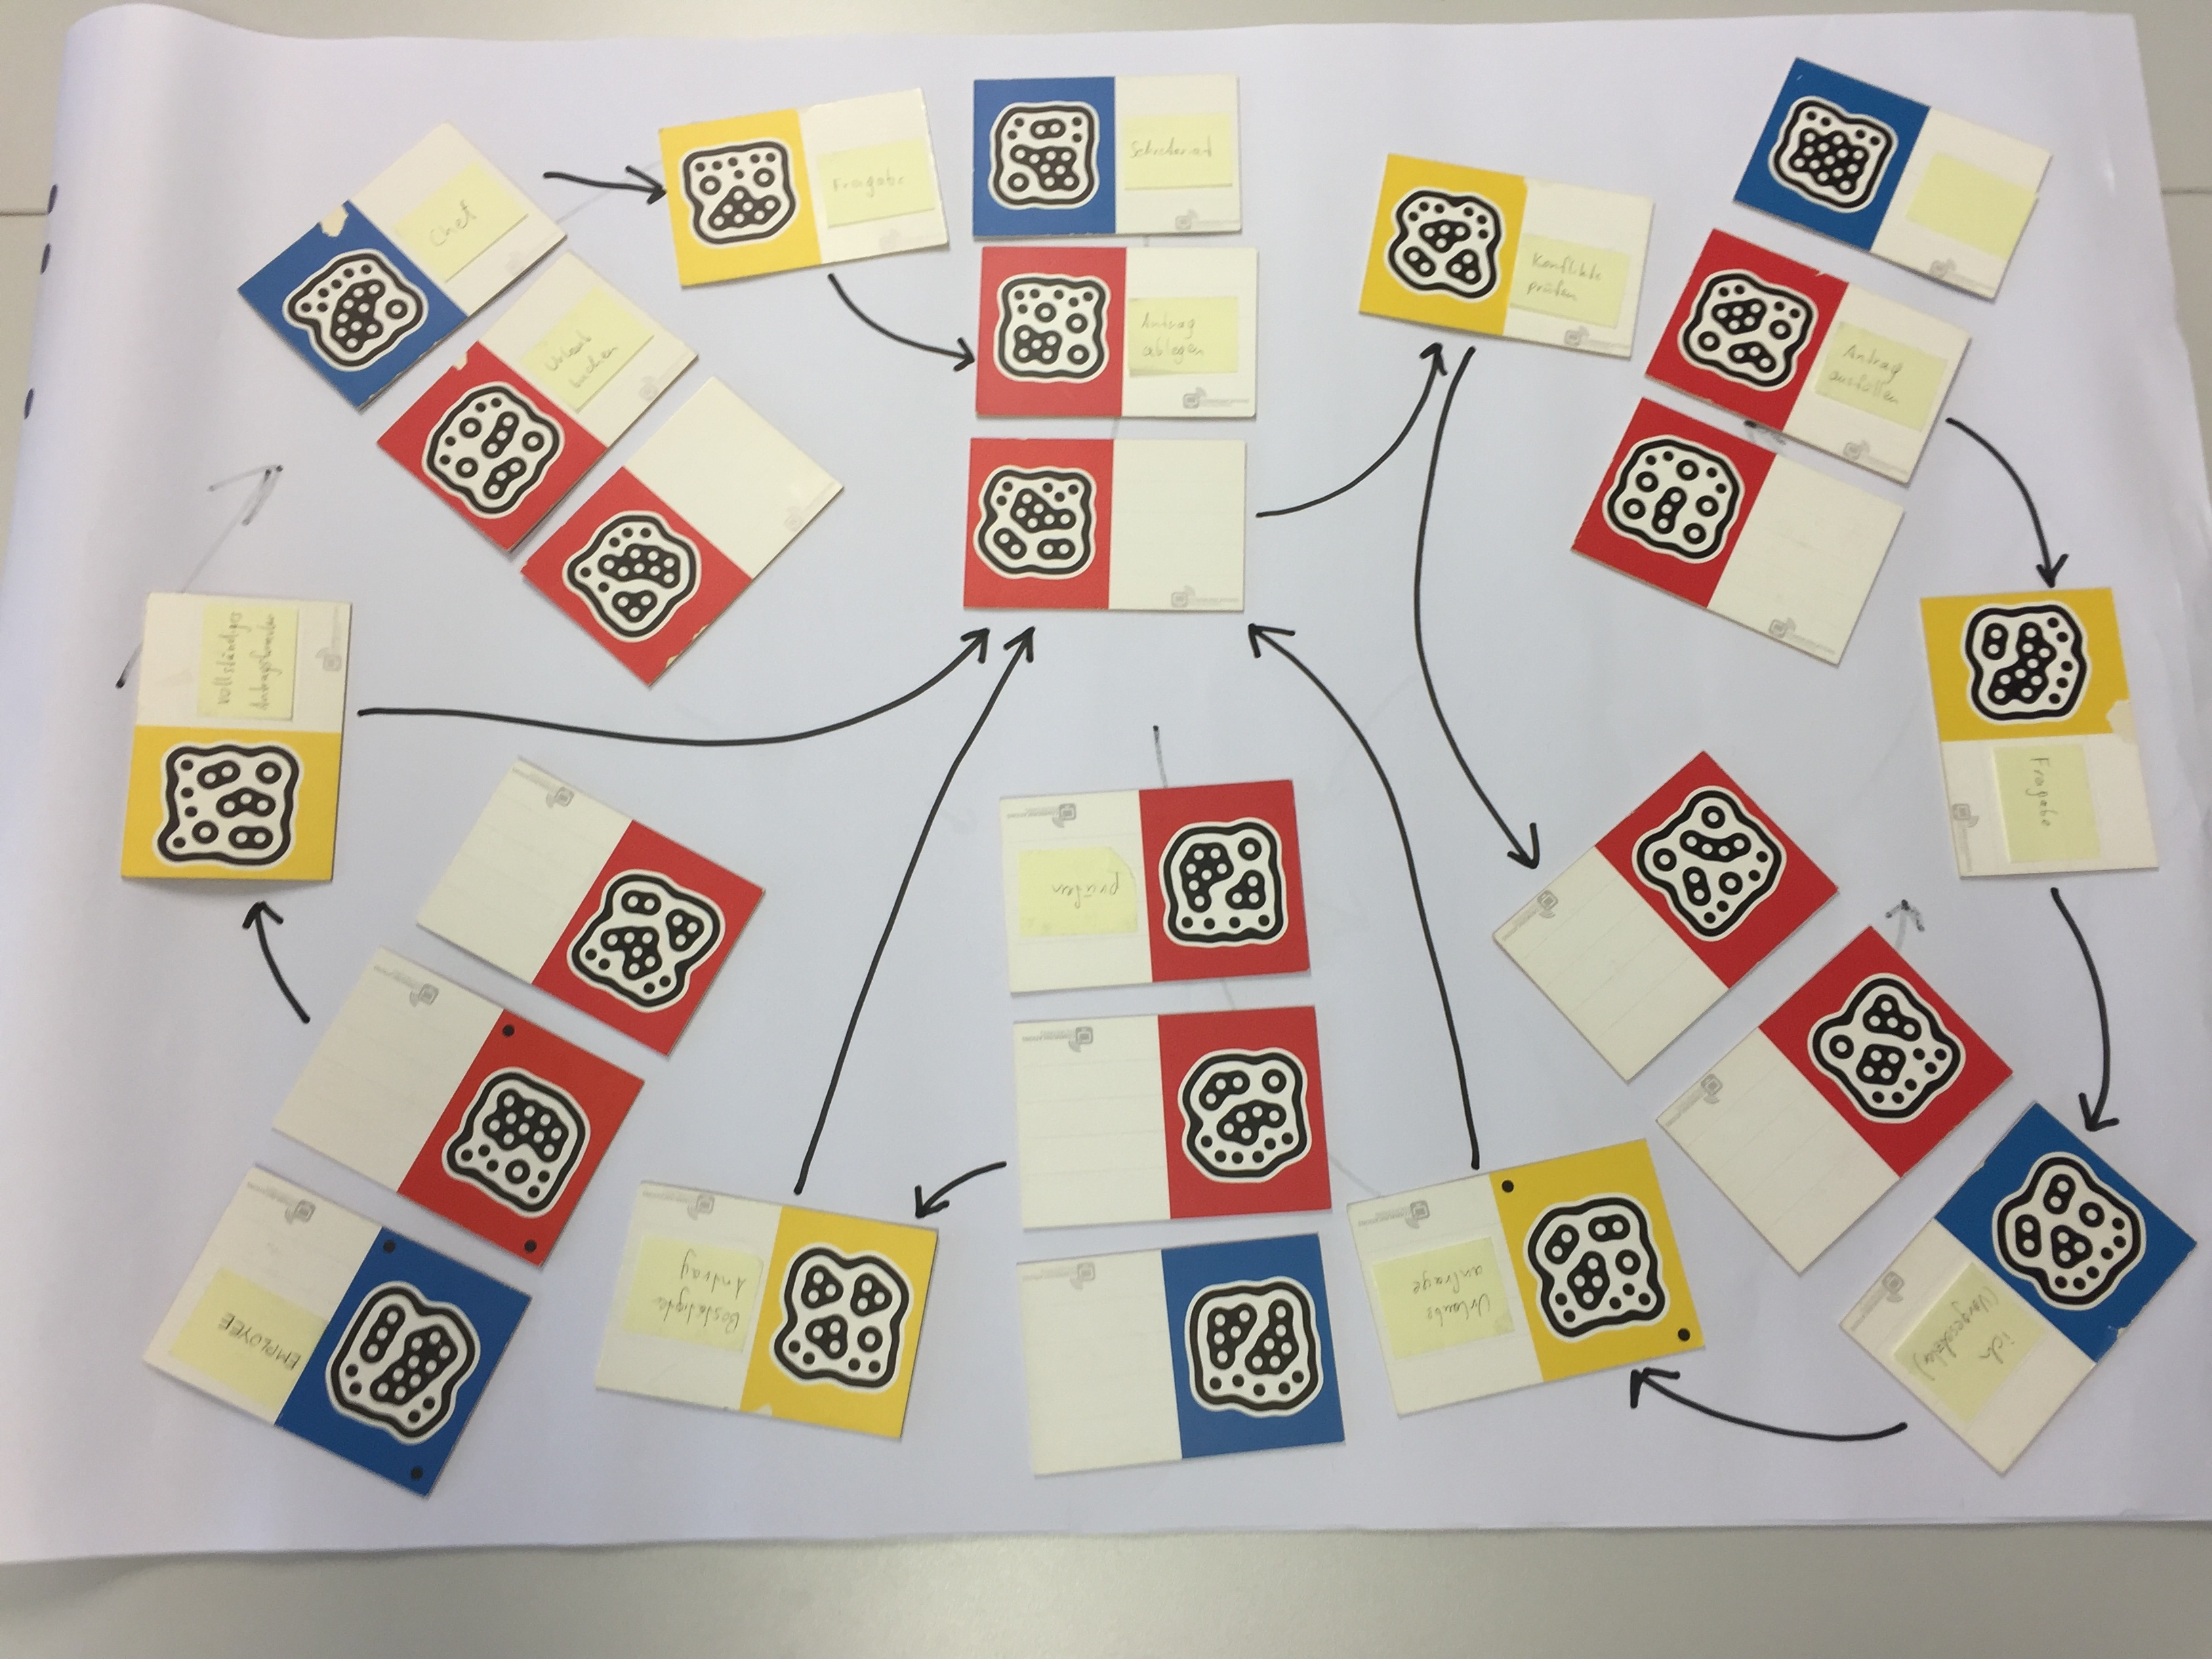
\includegraphics[width=\linewidth]{figures/11.jpg} & Ja & Entspricht in Bezug auf den Algorithmus Testfall 10.  \\
		\midrule
		12 & 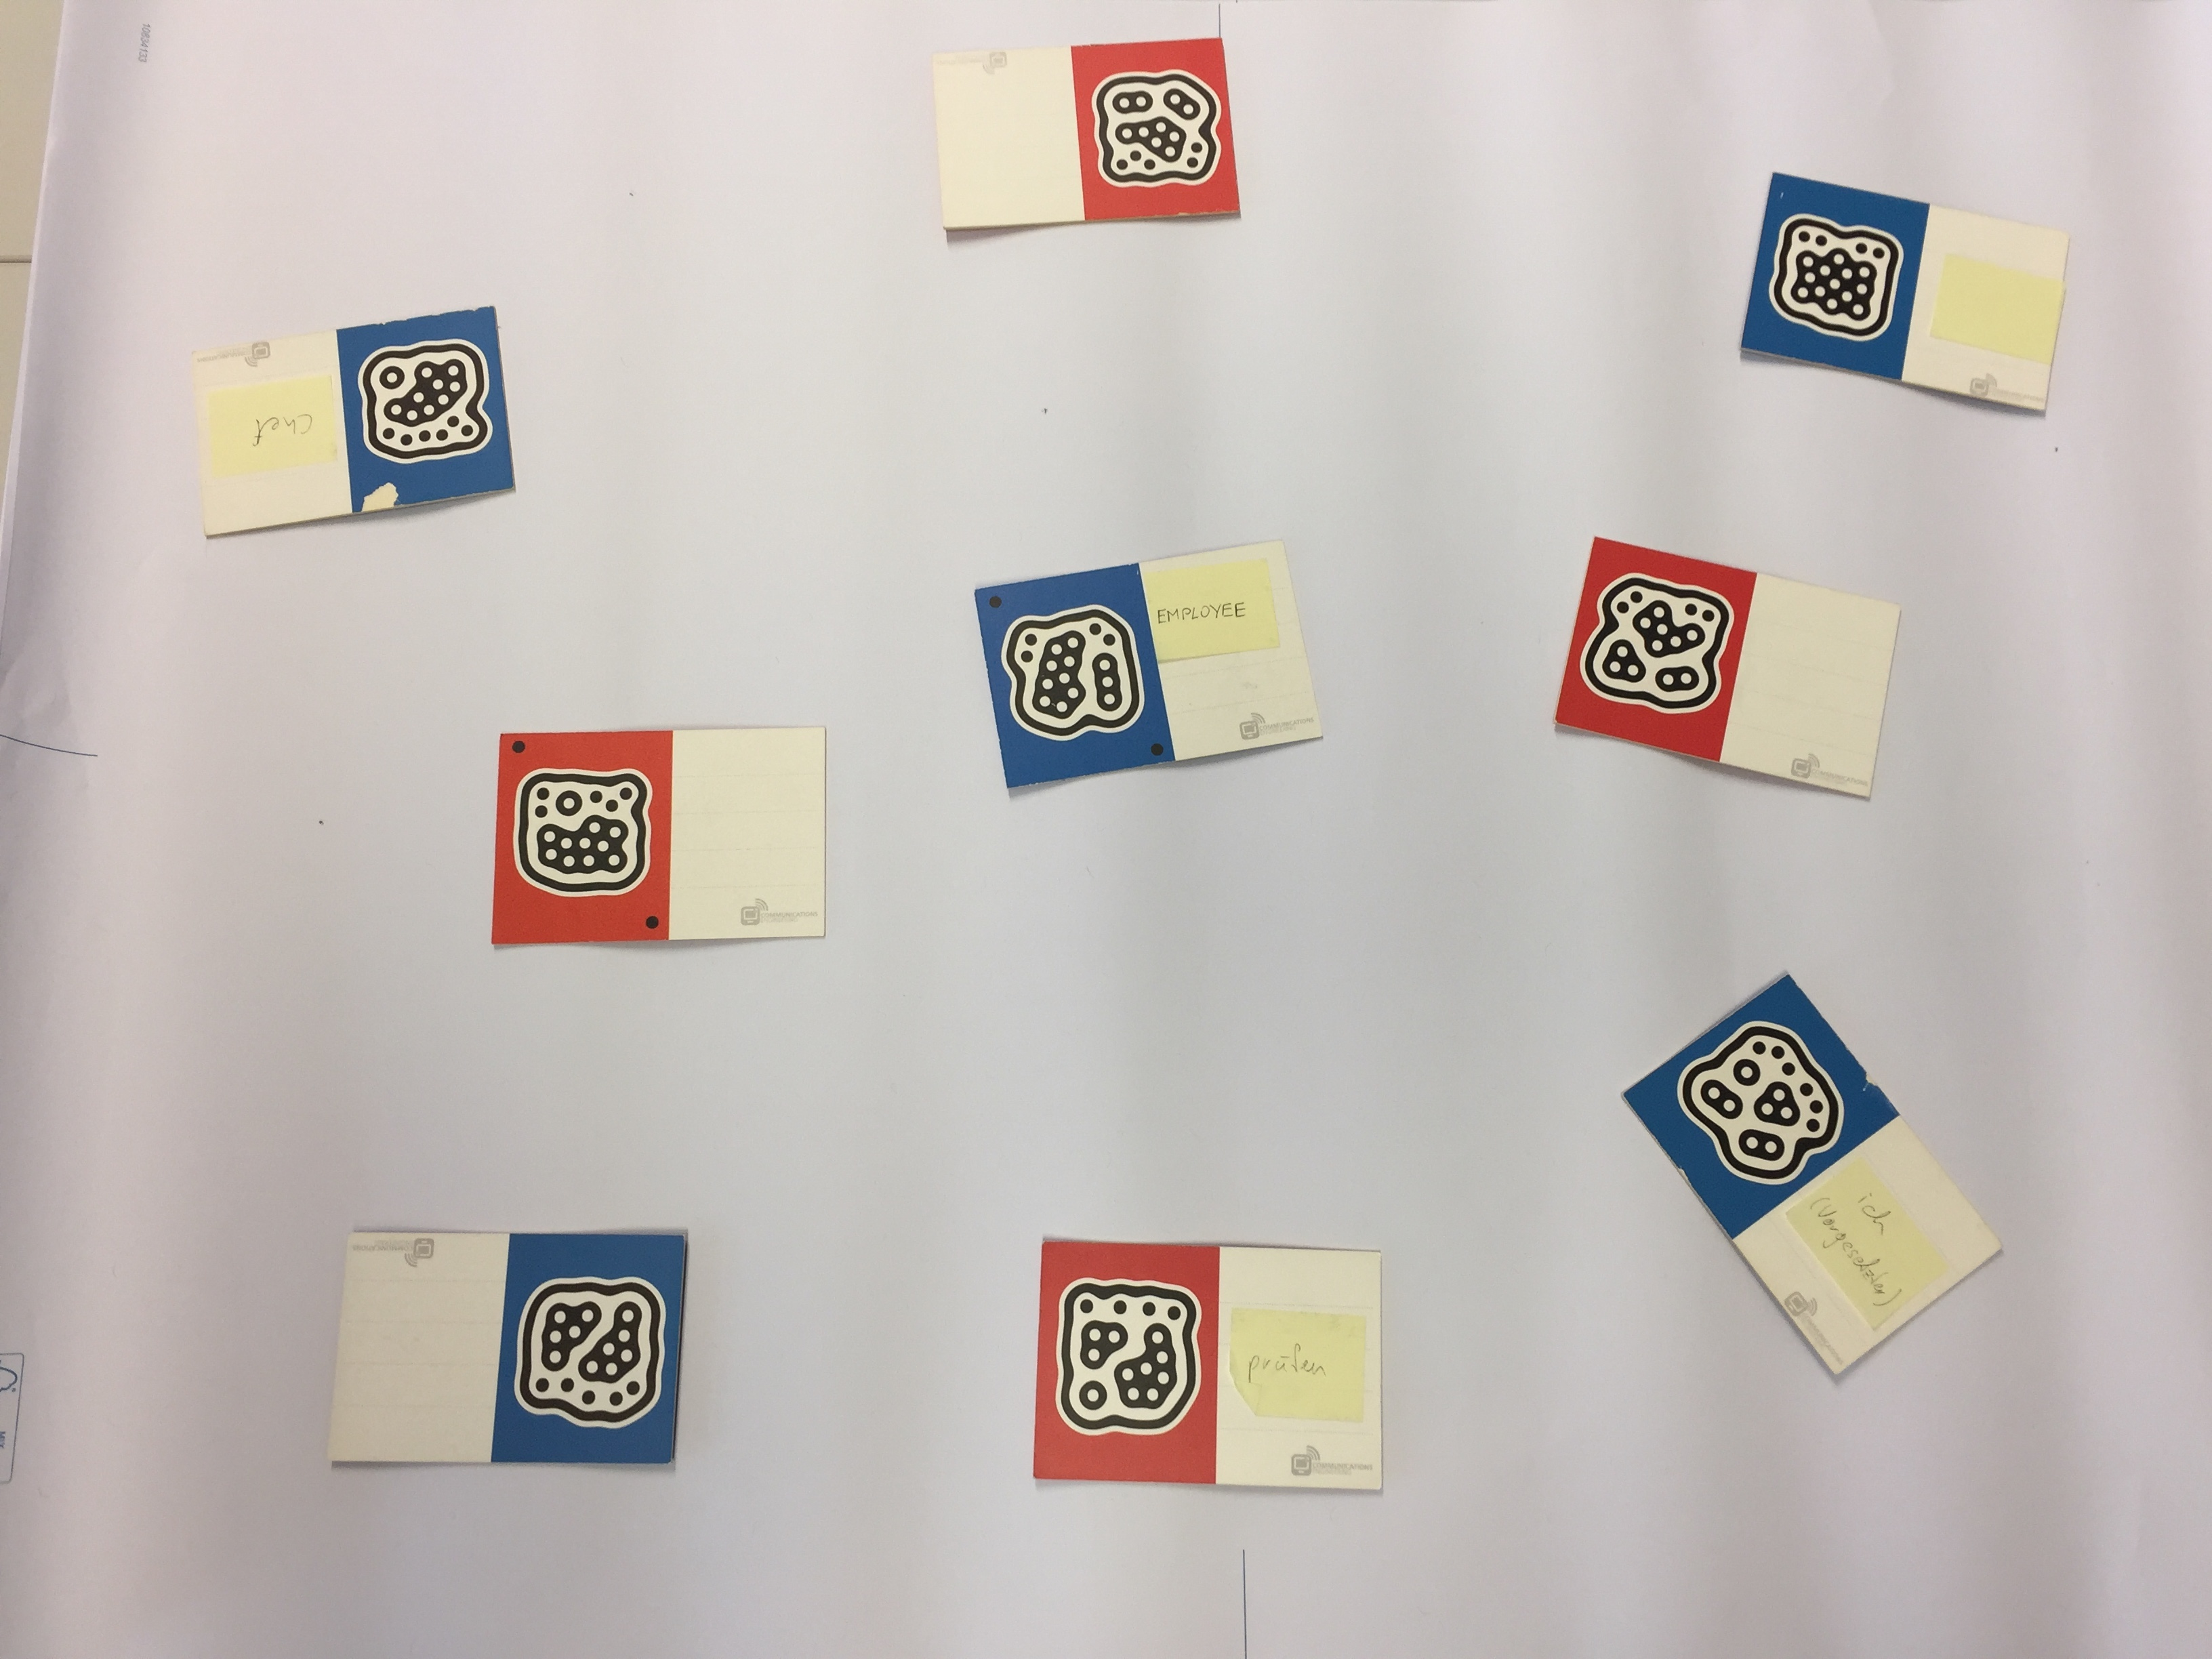
\includegraphics[width=\linewidth]{figures/12.jpg} & Ja & Der Testfall wird als Sternmuster erkannt. \\
		\midrule
		13 & 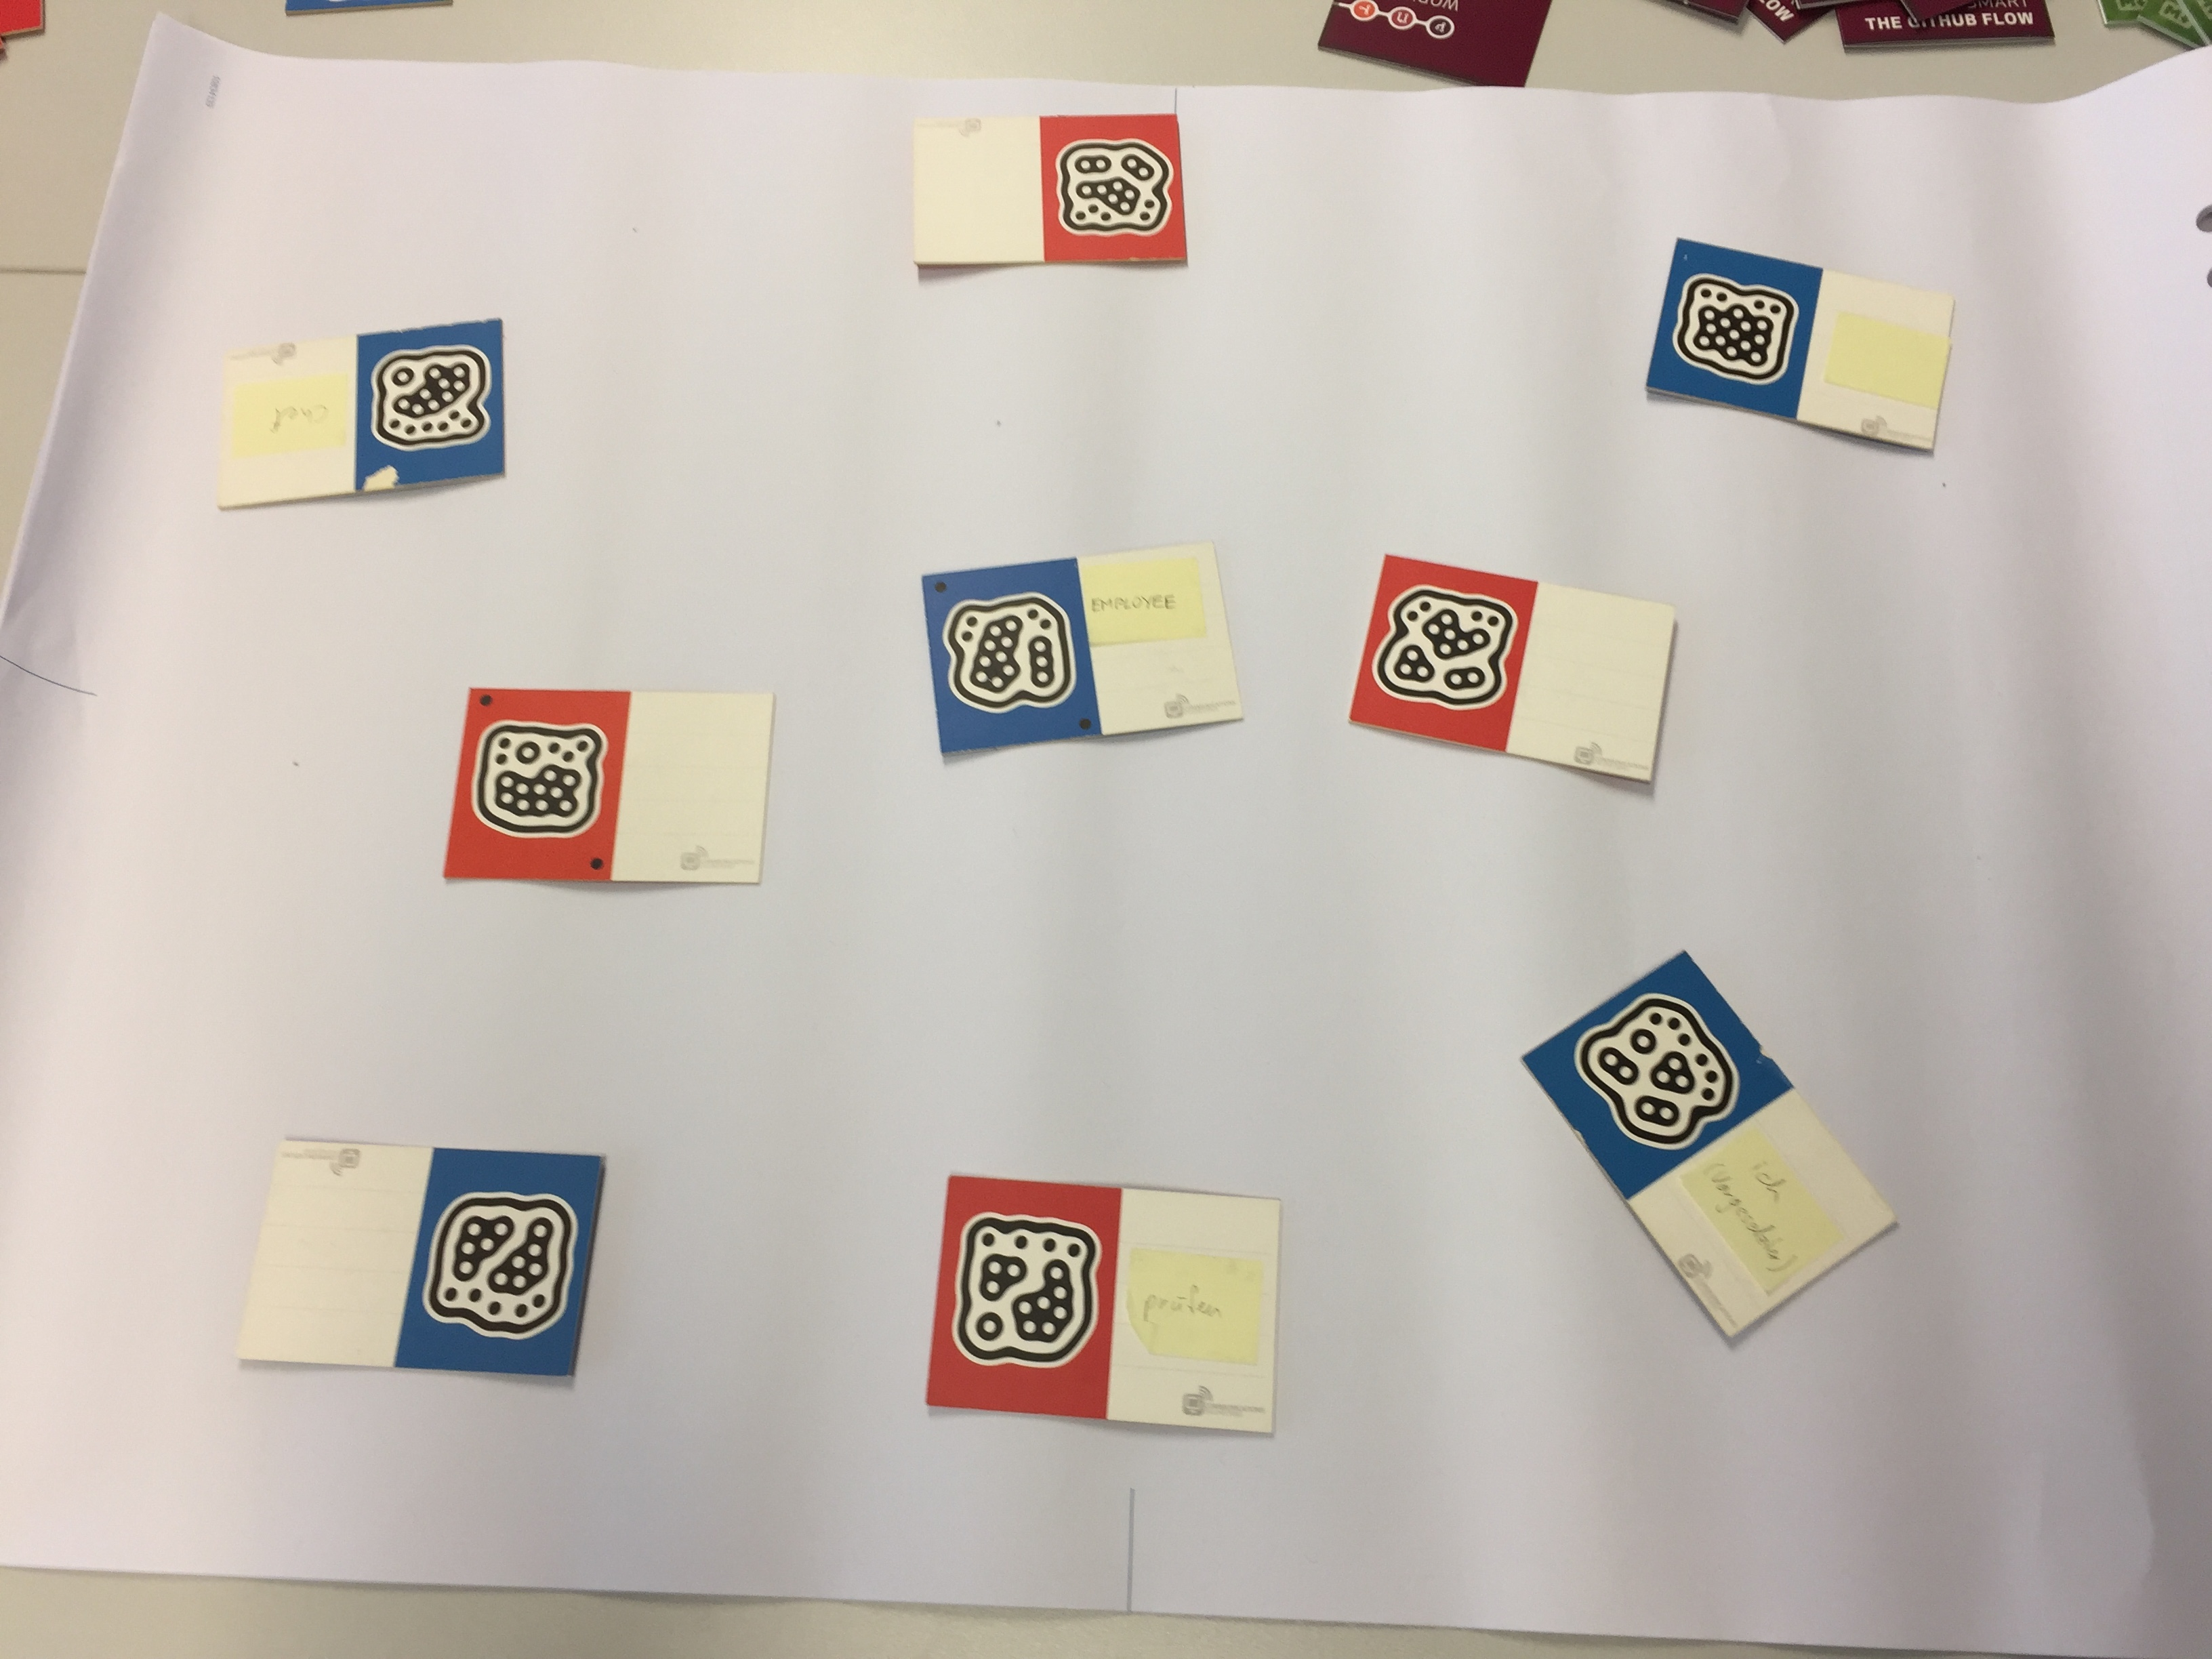
\includegraphics[width=\linewidth]{figures/13.jpg} & Ja & Der Testfall wird als Sternmuster erkannt. \\
		\midrule
		14 & 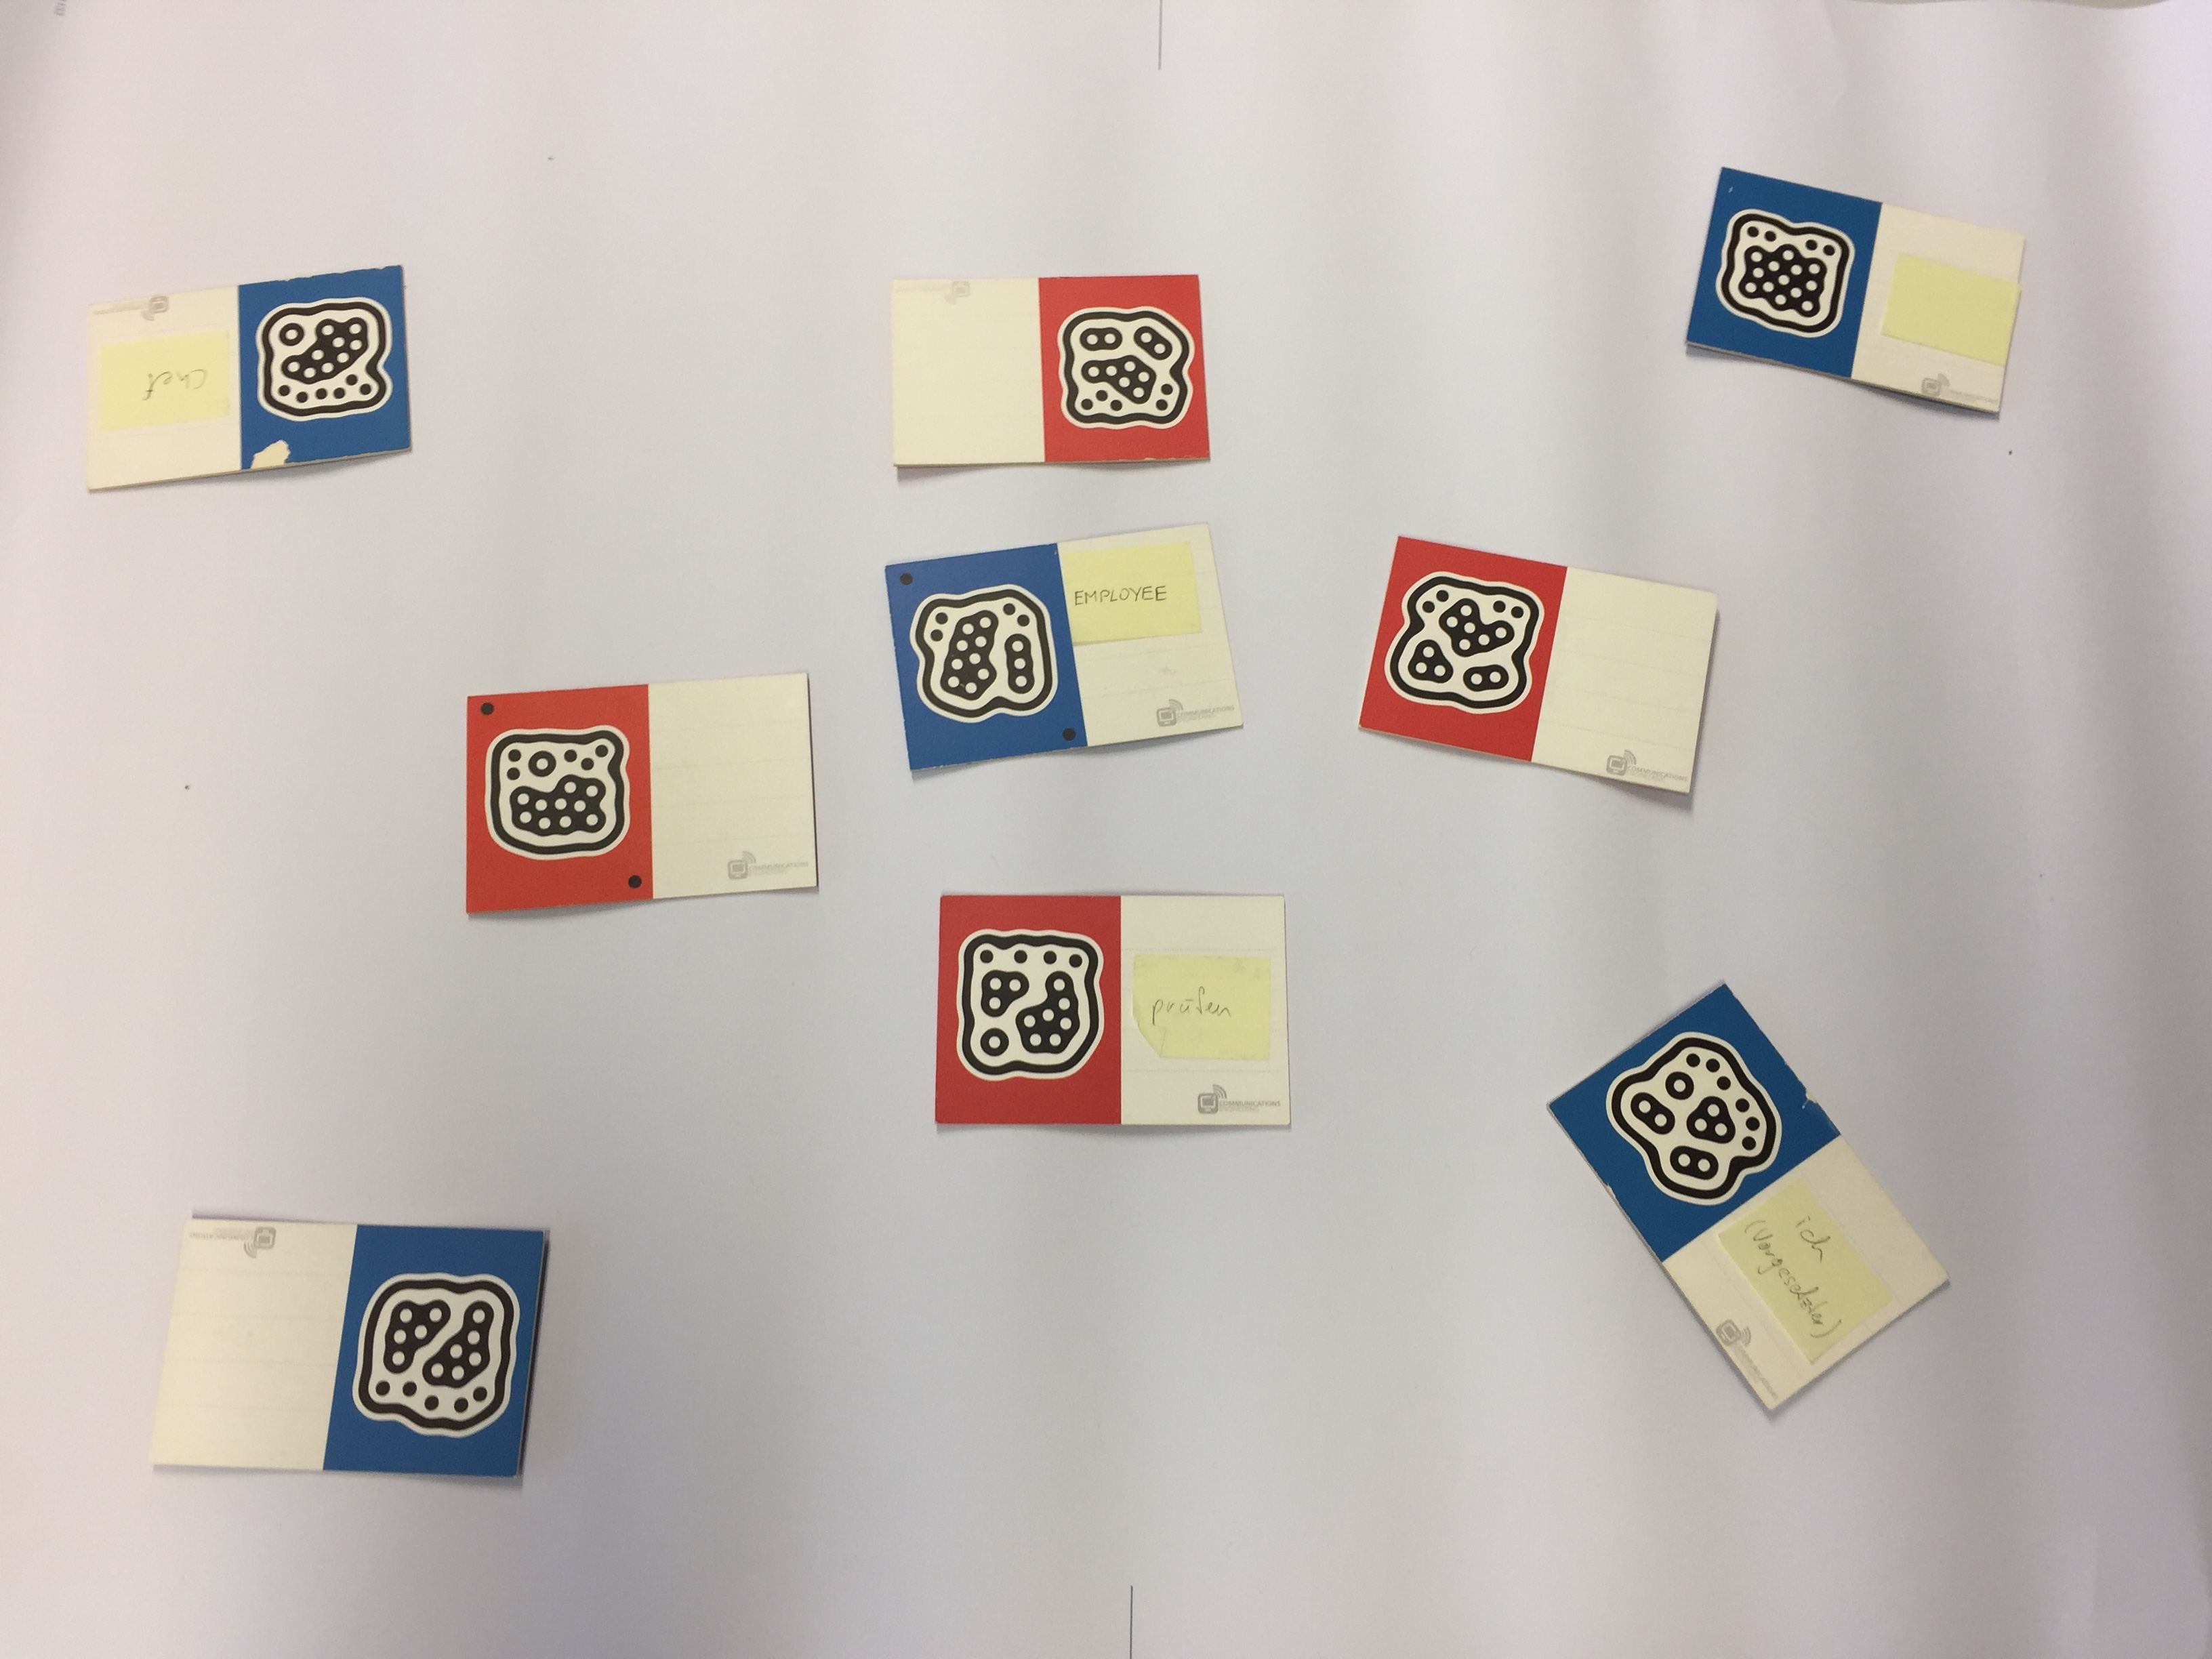
\includegraphics[width=\linewidth]{figures/14.jpg} & Ja & Der Testfall wird als Sternmuster erkannt. \\
		\midrule
		15 & 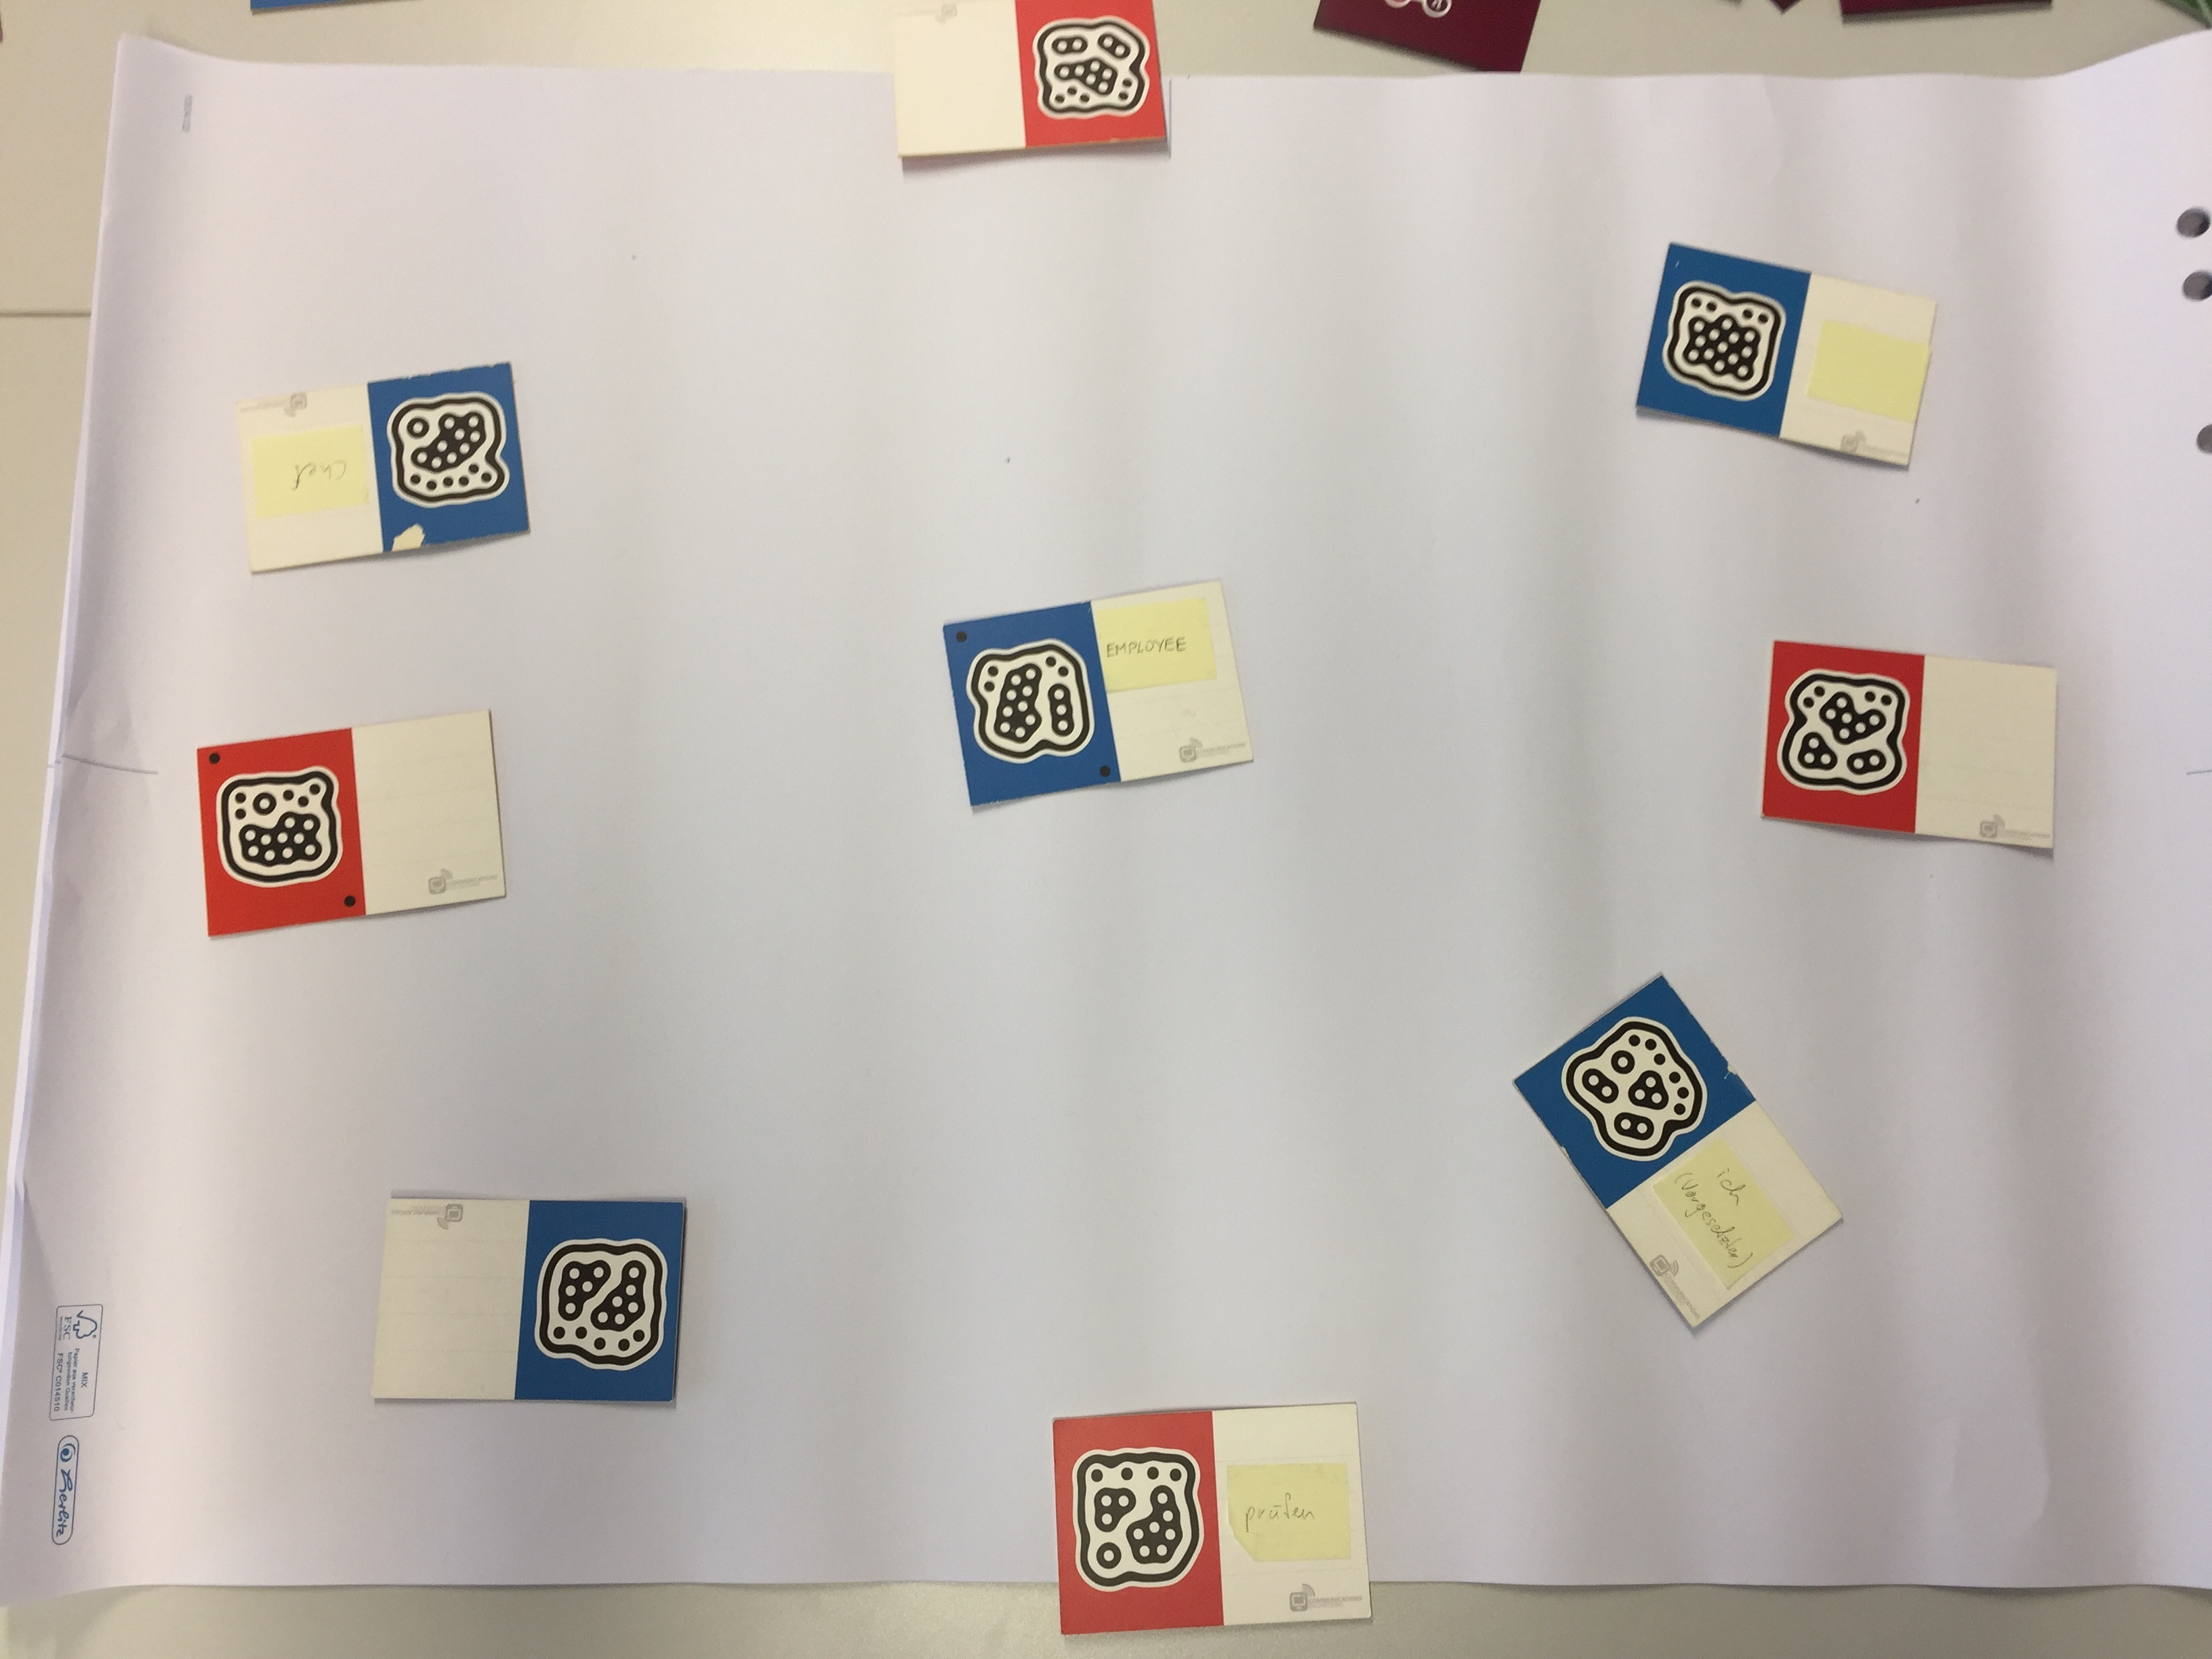
\includegraphics[width=\linewidth]{figures/15.jpg} & Ja & Der Testfall wird als Sternmuster erkannt. \\
		\midrule
		16 & 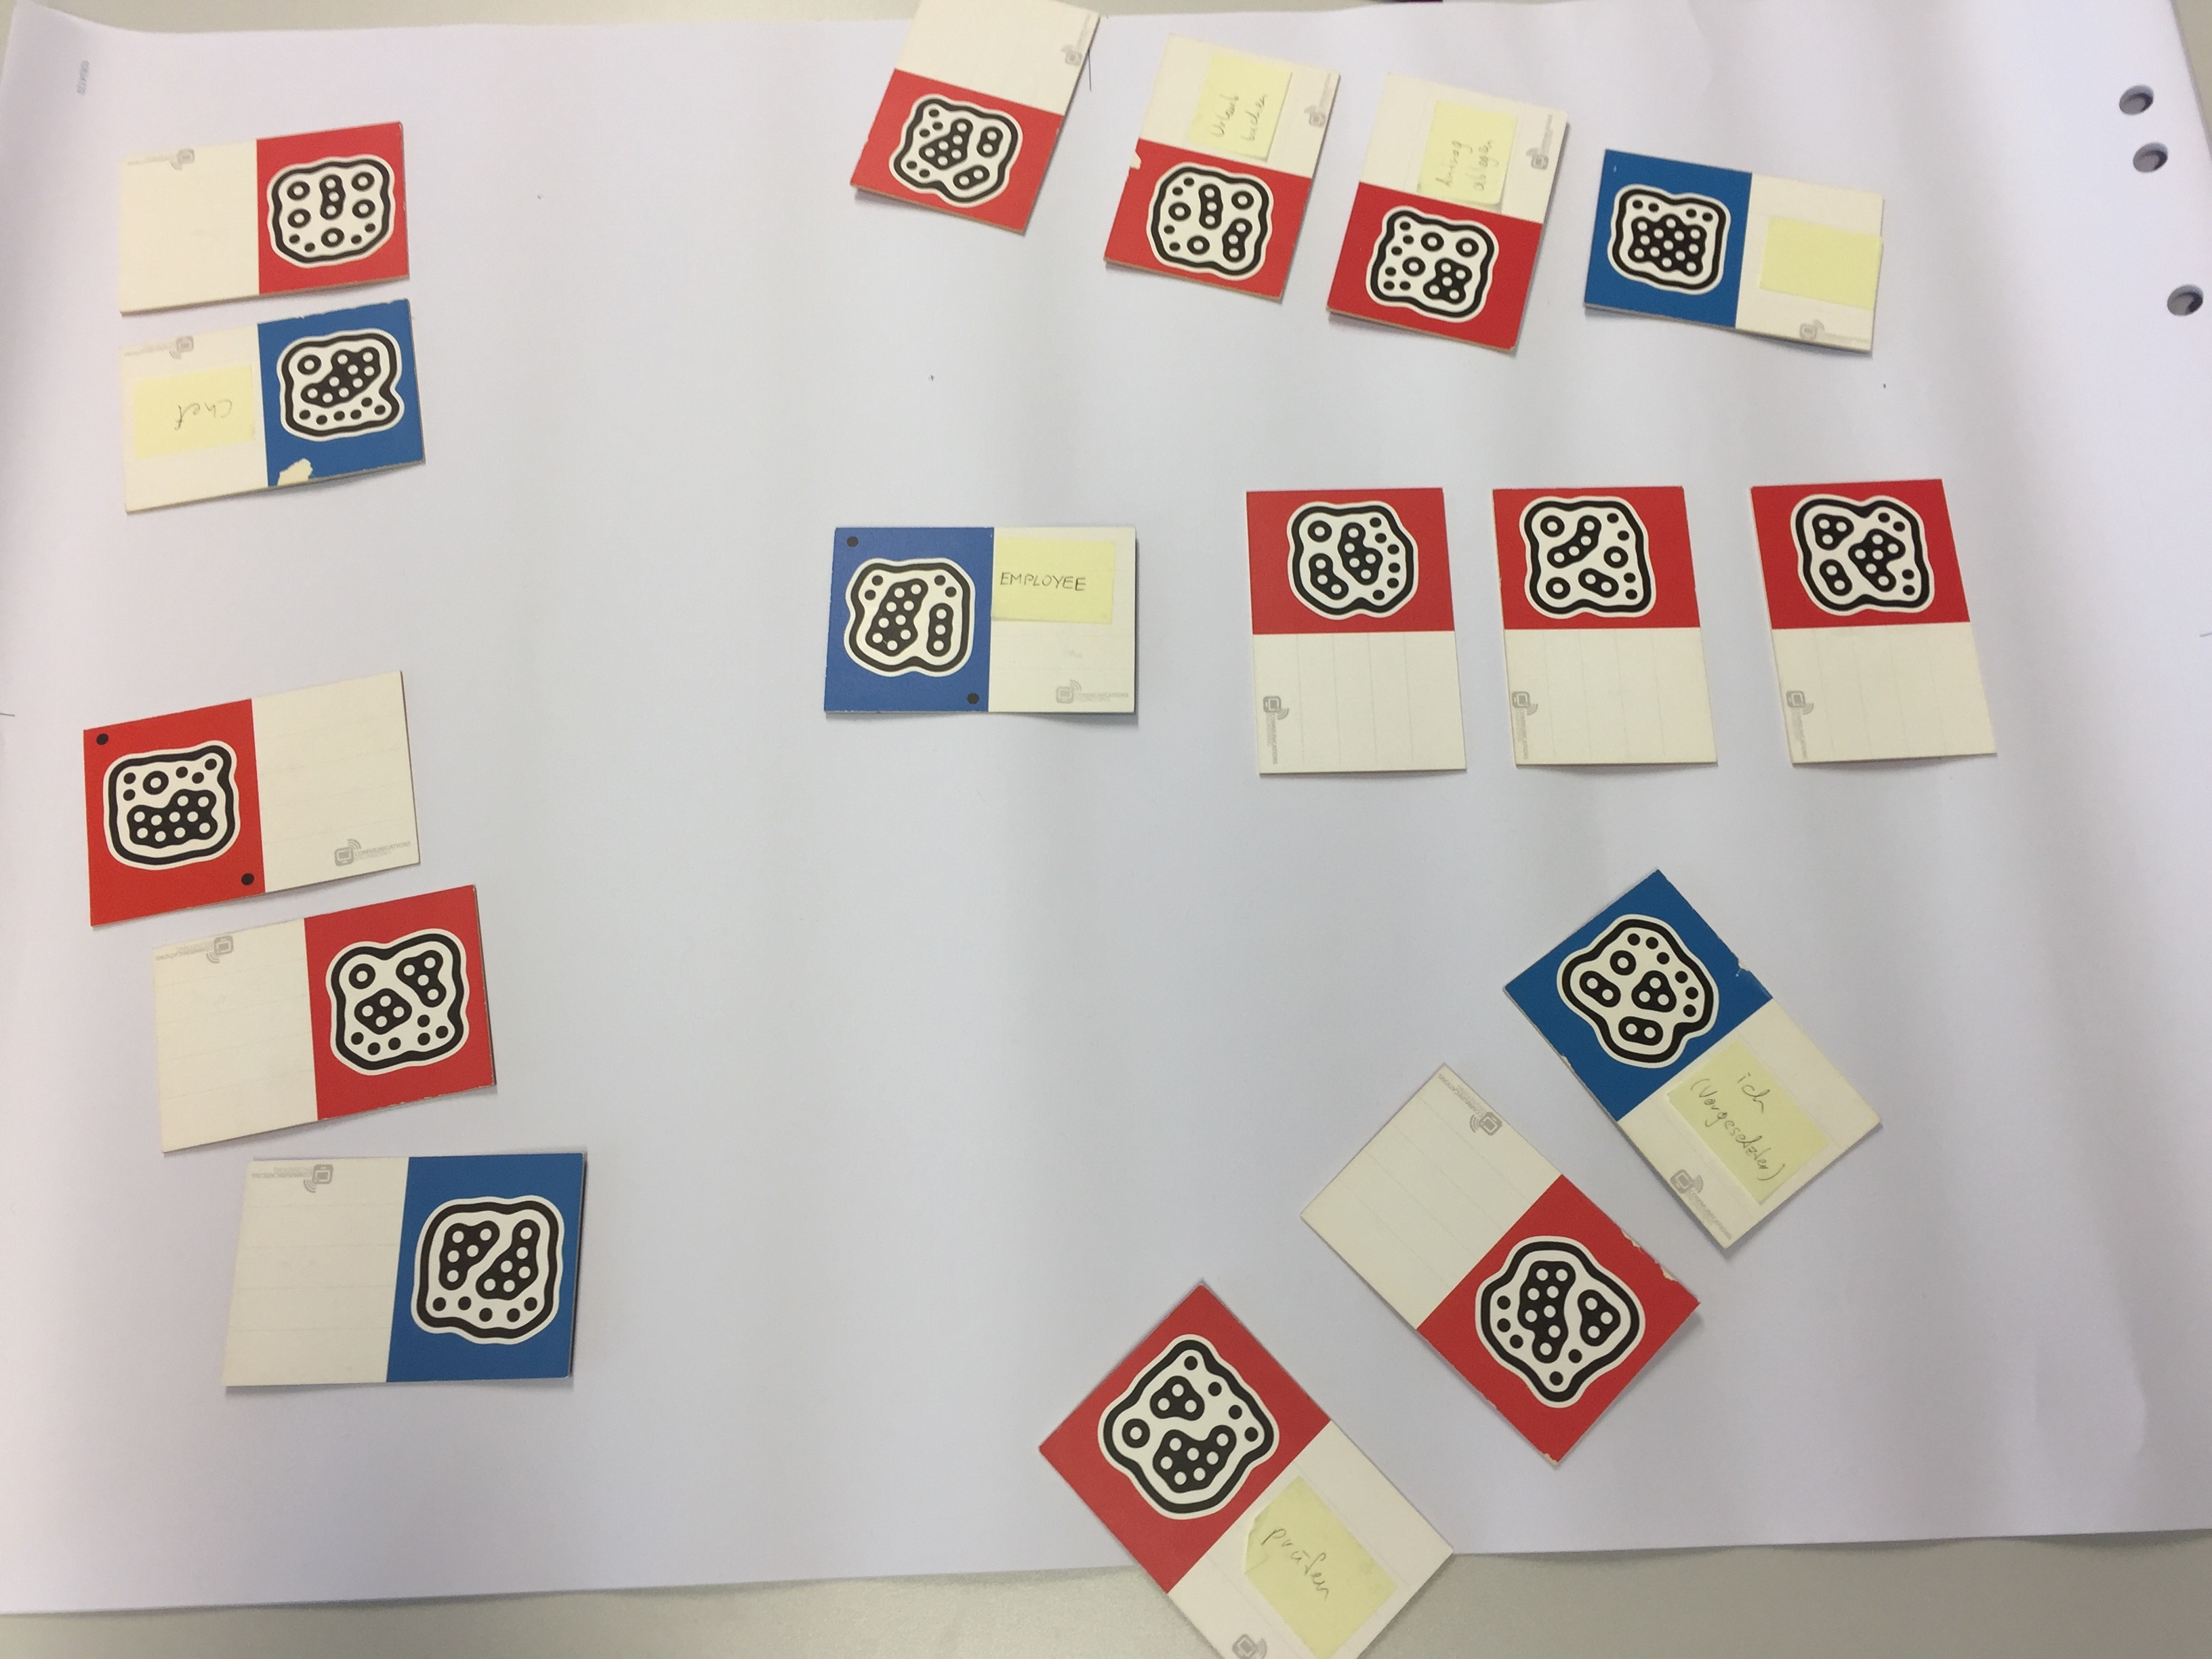
\includegraphics[width=\linewidth]{figures/16.jpg} & Ja & Dieses Beispiel zeigt, dass trotz unterschiedlicher Richtungen die Zuordnungen richtig erkannt werden \\
		\midrule
		17 & 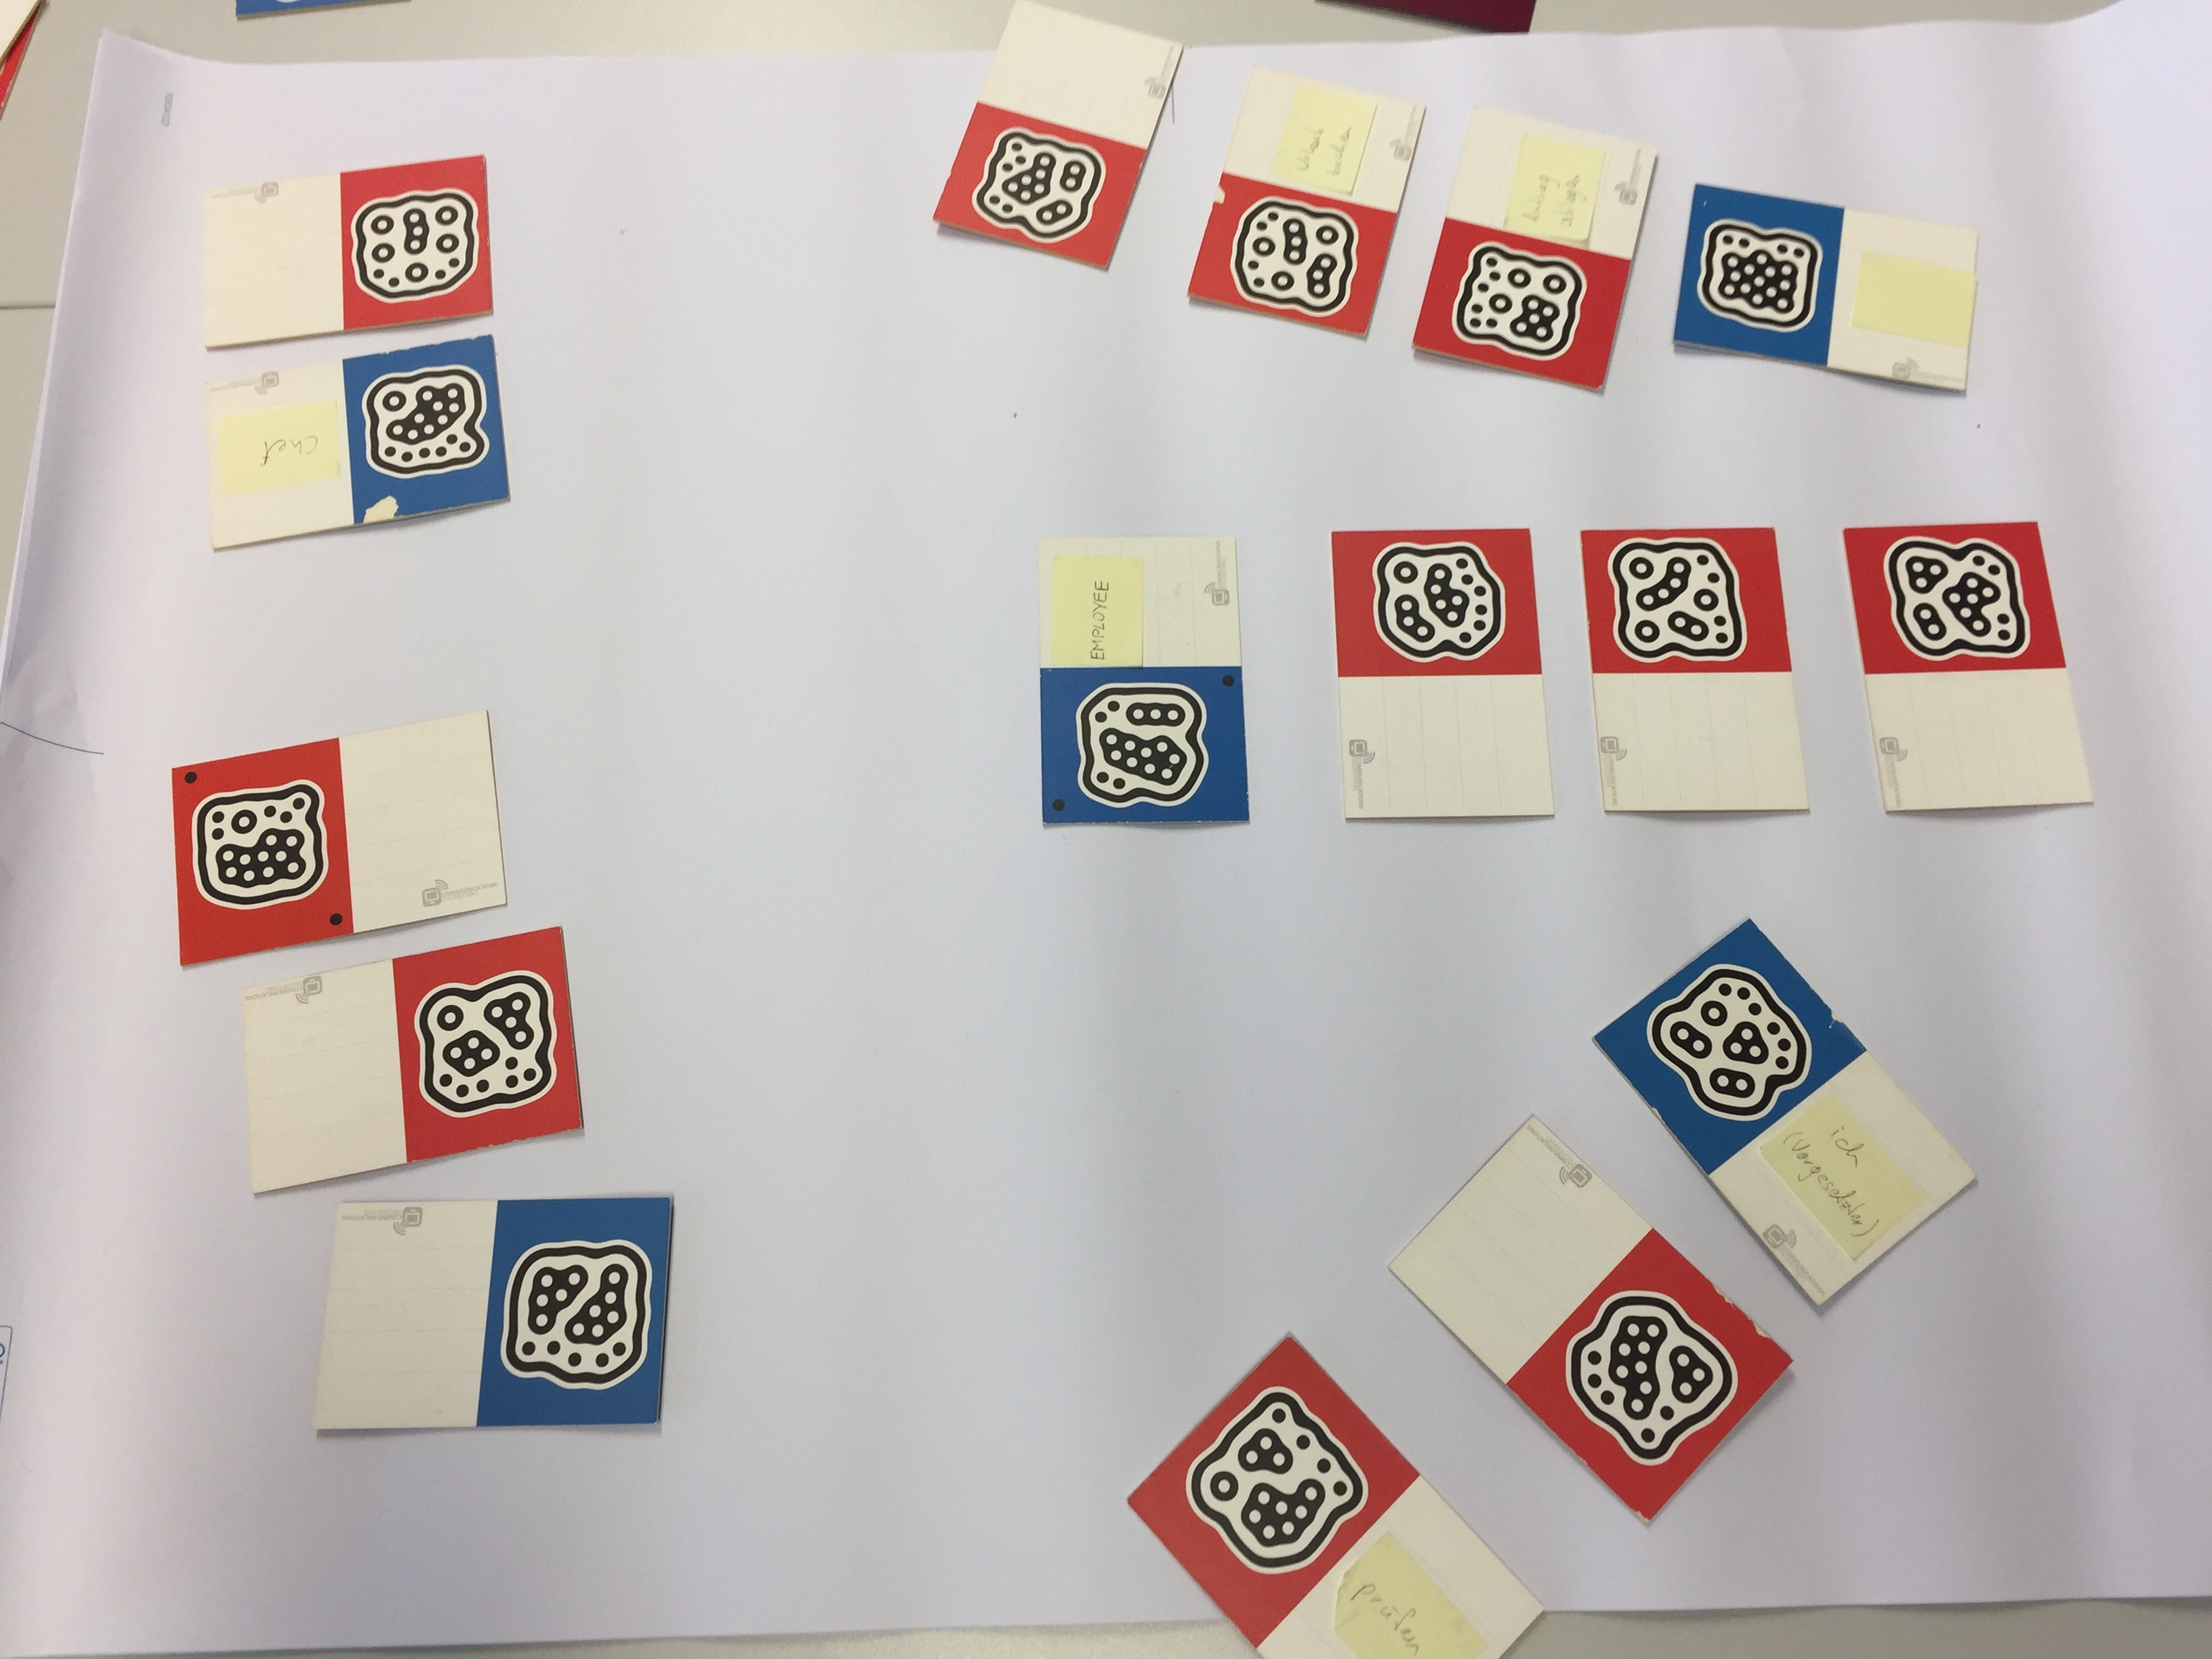
\includegraphics[width=\linewidth]{figures/17.jpg} & Ja & Entspricht in Bezug auf den Algorithmus Testfall 16. \\
		\midrule
	\end{longtabu}
\end{center}
}

Die Ergebnisse zeigen, dass der Algorithmus für alle Testfälle fehlerfrei funktioniert.



%----------------------------------------------------------------
%
%  File    :  thesis-style.tex
%
%  Author  :  Keith Andrews, IICM, TU Graz, Austria
% 
%  Created :  27 May 93
% 
%  Changed :  19 Feb 2004
% 
% styling and technical implementation adopted 2011 by Karl Voit
%----------------------------------------------------------------

%% defined an anvironment for the style Keith used to use:

\chapter{Diskussion und Future Work}
\label{chap:Diskussion}
In Kapitel \ref{cha:Empfehlungen} wurde die Relevanz von CBM bezüglich der Verständlichkeit nach \citet{MENDLING2010127} gezeigt. Kapitel \ref{cha:hintergrund} zeigt die grundsätzliche Funktionsweise von CBM. Basierend auf CBM wurden in Kapitel \ref{cha:erkennung} die Kriterien für die Interpretation von gelegten Prozessmodellen bestimmt, welche in Kapitel \ref{sec:erkennungsstrategie} zur Formulierung einer Erkennungsstrategie verwendet wurden. Aus diesen Erkenntnissen wurde in Kapitel \ref{cap:algorithmus} der Algorithmus entwickelt, welcher in Kapitel \ref{chap:Ergebnisse} anhand von Testfällen verifiziert wurde. 

Die Ergebnisse zeigen, dass der vorgestellte Algorithmus die Anforderungen erfüllt und eine verbesserte Zuverlässigkeit im Vergleich zu \citet{max} feststellbar ist. Alle Testfälle wurden den Erwartungen entsprechend erkannt. Damit bildet der Algorithmus die Basis für weitere Schritte in der Digitalisierung von Prozessmodellen nach CBM. Zur vollständigen Überleitung in ein ausführbares S-BPM Modell müsste der Algorithmus um die Erkennung der Austauschelemente und deren Beziehungen erweitert werden. 


%% include tex file chapters:
% \include{introduction}        %% this is a suggestion: you have to create this file on demand
% \include{problem}             %% this is a suggestion: you have to create this file on demand
% \include{solution}            %% this is a suggestion: you have to create this file on demand
% \include{evaluation}          %% this is a suggestion: you have to create this file on demand
% \include{outlook}             %% this is a suggestion: you have to create this file on demand

\appendix                       %% closes main document, appendix follows until end; only available in book-classes
%\addpart*{Appendix}             %% adding Appendix to tableofcontents

\printbibliography              %% remove, if using BibTeX instead of biblatex
% \include{further_ressources}  %% this is a suggestion: you have to create this file on demand






%%%% end{document}
\end{document}
%% vim:foldmethod=expr
%% vim:fde=getline(v\:lnum)=~'^%%%%\ .\\+'?'>1'\:'='
%%% Local Variables:
%%% mode: latex
%%% mode: auto-fill
%%% mode: flyspell
%%% eval: (ispell-change-dictionary "en_US")
%%% TeX-master: "main"
%%% End:
